\documentclass[journal]{IEEEtran}

% ============================================================
% PREÂMBULO: PACOTES E CONFIGURAÇÕES
% ============================================================

% --- CODIFICAÇÃO E IDIOMA ---
\usepackage[utf8]{inputenc}
\usepackage[brazilian]{babel}

% --- MATEMÁTICA ---
\usepackage{amsmath, amssymb, amsfonts}
\usepackage{mathrsfs}

% --- FIGURAS E TABELAS ---
\usepackage{graphicx}
\usepackage{booktabs}
\usepackage{float}
\usepackage{multirow}
\usepackage[table]{xcolor}
\usepackage{subcaption}

% --- UTILITÁRIOS ---
\usepackage{cite}
\usepackage{siunitx}        
\usepackage[
    colorlinks=true,
    linkcolor=blue!70!black,
    citecolor=green!50!black,
    urlcolor=blue!80!black,
    pdfborder={0 0 0},
]{hyperref}   
\usepackage{url}            
\usepackage{siunitx}
\sisetup{output-decimal-marker = {,}, retain-explicit-plus = true}

% --- PSEUDOCÓDIGO ---
\usepackage{algorithm}
\usepackage{algpseudocode}

% ============================================================
% CONFIGURAÇÃO DO DOCUMENTO
% ============================================================

\title{Rastreamento Bidimensional de Alvos via Filtro de Kalman Estendido em Sistemas de Posicionamento por Estações Base}

\author{Saulo José Almeida Silva,~\IEEEmembership{Mestrando,~UFCG,}%
        \thanks{S. J. A. Silva é mestrando no Programa de Pós-Graduação em Engenharia Elétrica (PPgEE) da Universidade Federal de Campina Grande (UFCG), Campina Grande, PB, Brasil. E-mail: saulo.jose.silva@ee.ufcg.edu.br.}}

% CABEÇALHO (Ajustado para refletir o tema real do seu trabalho)
\markboth{PROCESSAMENTO ADAPTATIVO DE SINAIS, 2026. PPgEE. CEEI.}%
{Silva \MakeLowercase{\textit{et al.}}: Rastreamento via EKF com Medições \textit{Range-Only}}

% ============================================================
% DOCUMENTO PRINCIPAL
% ============================================================

\begin{document}

\maketitle

% --- RESUMO E PALAVRAS-CHAVE ---
\begin{abstract}
A localização precisa é um requisito fundamental para a operação autônoma de sistemas robóticos móveis. Este trabalho apresenta o desenvolvimento, a implementação e a análise rigorosa de um Filtro de Kalman Estendido (EKF) aplicado ao rastreamento bidimensional de alvos utilizando medições não lineares de distância (\textit{range-only}). Fundamentado em um modelo cinemático de Posição-Velocidade-Aceleração (PVA), o estimador foi avaliado por meio de um ambiente de simulação em Python. A arquitetura viabiliza o monitoramento contínuo da acurácia posicional (RMSE), da consistência estatística via \textit{Normalized Innovation Squared} (NIS) e da validação espacial de crença através da Taxa de \textit{Inliers}. Os resultados demonstram que, sob sintonia adequada das matrizes de processo ($\mathbf{Q}$) e medição ($\mathbf{R}$), o EKF atinge precisão submétrica e robustez contra oclusões temporárias. Em contraste, a descalibração paramétrica revela um desacoplamento perigoso: subestimar $\mathbf{R}$ gera falsas altas taxas de \textit{inliers} enquanto corrompe o NIS, e subestimar $\mathbf{Q}$ induz a atrasos de fase severos. Conclui-se que cruzar métricas geométricas e estatísticas é imperativo para atestar a verdadeira confiabilidade do filtro.
\end{abstract}

\begin{IEEEkeywords}
Filtro de Kalman Estendido, Localização em Tempo Real, Posicionamento \textit{Range-Only}, Consistência Estatística.
\end{IEEEkeywords}

\IEEEpeerreviewmaketitle

% ============================================================
% INCLUSÃO DOS CAPÍTULOS
% ============================================================

% Capítulo 1: Introdução
% ============================================================
% CAPÍTULO 1: INTRODUÇÃO
% ============================================================

\section{Introdução}
\label{sec:introduction}

\IEEEPARstart{A}{o} passo que os sistemas robóticos autônomos assumem tarefas mais complexas, cresce também a exigência por soluções de navegação precisas e confiáveis. Para mitigar as incertezas inerentes a esse processo, a literatura tem apostado fortemente em arquiteturas de fusão sensorial — que combinam dados de múltiplos sensores — associadas a análises estatísticas das medições. Essa integração tem se mostrado essencial para refinar a estimativa de estado do sistema e viabilizar sua aplicação no mundo real \cite{odry2018kalman, reina2007adaptive}.

O grande desafio no desenvolvimento dessas soluções de localização está nos erros instrumentais e nos ruídos estocásticos que afetam a dinâmica do robô. Mesmo sob uma modelagem cinemática detalhada, perturbações ambientais e não-linearidades — presentes tanto na resposta física dos sensores quanto na própria dinâmica veicular — acabam inserindo margens inevitáveis de imprecisão no estado estimado.

Para contornar essa limitação e obter estimativas de alta fidelidade, utiliza-se o Filtro de Kalman (KF), um estimador ótimo iterativo para sistemas lineares sob o critério do erro quadrático mínimo \cite{kalman1960new}. Como parte da família dos filtros bayesianos, o KF estima variáveis de estado não mensuradas diretamente, o que viabiliza sua aplicação em cenários de observabilidade incompleta \cite{thrun2005probabilistic}. Essa formulação clássica, no entanto, é limitada em sistemas de posicionamento baseados em distância (alcance), cujas equações de observação são essencialmente não-lineares. Nesses cenários, aplica-se o Filtro de Kalman Estendido (EKF), que contorna a não linearidade por meio da linearização do modelo em torno da estimativa corrente \cite{thrun2005probabilistic, chen2012kalman}.

Embora o EKF possua uma fundamentação teórica consolidada, seu sucesso prático depende diretamente do ajuste das matrizes de covariância do processo ($\mathbf{Q}$) e de medição ($\mathbf{R}$). A sintonia desses parâmetros requer simulações computacionais detalhadas, etapa essencial no desenvolvimento de sistemas de navegação. Um exemplo dessa abordagem é o trabalho de Falek e Kaniewski \cite{falek2020computer}, que propuseram um ambiente em MATLAB para avaliar o comportamento do EKF em redes de posicionamento baseadas em estações fixas.

Nesse contexto, este trabalho apresenta um simulador em Python voltado à análise do rastreamento bidimensional de alvos via quatro estações base. A ferramenta integra uma GUI interativa para avaliar a acurácia posicional (RMSE), a consistência estatística (NIS) e o comportamento da crença do robô (Taxa de \textit{Inliers}). Para detalhar essa abordagem, o artigo está estruturado da seguinte forma: a Seção II revisa a fundamentação do EKF; a Seção III detalha a modelagem cinemática proposta; a Seção IV descreve a metodologia e as métricas de validação; a Seção V discute os resultados comparativos de sintonia; e a Seção VI apresenta as conclusões e trabalhos futuros.


\subsection{Notação e Convenções}
\label{subsec:notation}

Neste trabalho, adota-se a seguinte convenção de notação: escalares são representados por letras minúsculas em itálico ($a$), vetores por minúsculas em negrito ($\mathbf{a}$ ou $\hat{\mathbf{x}}$) e matrizes por maiúsculas em negrito ($\mathbf{A}$ ou $\mathbf{P}$).

No domínio discreto, o subscrito $k$ denota a variável física real no instante de tempo atual (como o estado $\mathbf{x}_k$ ou a medição $\mathbf{z}_k$). Por outro lado, os estados e as covariâncias calculados pelo estimador utilizam uma notação composta:
\begin{itemize}
    \item $k|k-1$: indica os valores \textit{a priori} (etapa de predição), computados a partir do histórico do sistema até o instante $k-1$, tais como o estado predito $\hat{\mathbf{x}}_{k|k-1}$ e a covariância do erro $\mathbf{P}_{k|k-1}$.
    \item $k|k$: representa os valores \textit{a posteriori} (etapa de correção), atualizados após a incorporação da nova medição, tais como o estado corrigido $\hat{\mathbf{x}}_{k|k}$ e a covariância do erro $\mathbf{P}_{k|k}$.
\end{itemize}

% Capítulo 2: Revisão Teórica
% ============================================================
% CAPÍTULO 2: REVISÃO TEÓRICA E TRABALHOS RELACIONADOS
% ============================================================
\section{Revisão Teórica e Trabalhos Relacionados}
\label{sec:theoretical}

Este capítulo apresenta a base teórica para o problema de estimativa de estados em robótica. O texto parte da modelagem determinística ideal e avança para os filtros probabilísticos usados na mitigação de incertezas em sistemas reais. Inicialmente, são apresentados os conceitos de sistemas dinâmicos e as fontes de ruído que afetam o comportamento do robô. Em seguida, introduz-se a definição de crença (\textit{belief}) sob a suposição de Markov, o que fundamenta a relação geométrica entre a matriz de covariância e a região de incerteza do agente. Por fim, são discutidos o modelo Gauss-Markov, a discretização temporal, as formulações do Filtro de Kalman (Linear e Estendido) e as métricas para validação do estimador.

\subsection{Sistemas Dinâmicos e Modelagem Determinística}
\label{subsec:dynamical_sys}

A modelagem de robôs móveis para navegação e controle costuma utilizar a representação em espaço de estados. No domínio do tempo contínuo, a evolução do vetor de estados ocultos $\mathbf{x}(t) \in \mathbb{R}^n$ e as medições ideais do sistema são descritas por equações diferenciais e algébricas \cite{ogata2010}, na forma:

\begin{equation}
    \label{eq:dinamica_continua}
    \dot{\mathbf{x}}(t) = f(\mathbf{x}(t), \mathbf{u}(t))
    \quad \text{e} \quad
    \mathbf{z}(t) = h(\mathbf{x}(t))
\end{equation}

onde $\mathbf{u}(t) \in \mathbb{R}^m$ é o vetor de entradas de controle e $\mathbf{z}(t) \in \mathbb{R}^d$ é o vetor de medições. Se as funções $f$ e $h$ forem lineares, o sistema pode ser escrito em sua forma canônica:

\begin{equation}
    \label{eq:sistema_linear_continuo}
    \dot{\mathbf{x}}(t) = \mathbf{A}_c \mathbf{x}(t) + \mathbf{B}_c \mathbf{u}(t)
    \quad \text{e} \quad
    \mathbf{z}(t) = \mathbf{H}_c \mathbf{x}(t)
\end{equation}

As matrizes $\mathbf{A}_c$, $\mathbf{B}_c$ e $\mathbf{H}_c$ definem a dinâmica, a entrada e a observação contínuas \cite{ogata2010}. Essa abordagem determinística assume sensores perfeitos e um modelo físico exato, desconsiderando os ruídos e distúrbios comuns em ambientes reais.

\subsection{Sistemas Estocásticos e Fontes de Incerteza}
\label{subsec:incertezas}

Na prática, os sistemas robóticos sofrem perturbações que inviabilizam o uso de modelos puramente determinísticos. Essas incertezas vêm de duas fontes principais \cite{reina2007adaptive}:

\begin{enumerate}
    \item \textbf{Ruído de Processo ($\boldsymbol{\epsilon}$):} Representa distúrbios dinâmicos, forças ambientais (como atrito variante, irregularidades no solo e correntes de ar) e erros de modelagem que afetam a locomoção do robô.
    \item \textbf{Ruído de Medição ($\boldsymbol{\delta}$):} Agrupa as incertezas dos próprios sensores. Em sistemas de localização por radiofrequência ou acústicos, decorre de efeitos de multicaminho, ruído térmico nos circuitos, atenuação de sinal e falhas de calibração \cite{barshalom2001estimation}.
\end{enumerate}

Com a inclusão desses ruídos, o estado deixa de ser um ponto exato e passa a ser tratado como uma variável aleatória. A evolução temporal do sistema e as leituras dos sensores passam a ser modeladas por densidades de probabilidade condicionais:

\begin{equation}
    \label{eq:prob_transicao}
    \mathbf{x}_k \sim P(\mathbf{x}_k \mid \mathbf{x}_{k-1}, \mathbf{u}_k)
\end{equation}
\begin{equation}
    \label{eq:prob_medicao}
    \mathbf{z}_k \sim P(\mathbf{z}_k \mid \mathbf{x}_k)
\end{equation}

onde $k \in \mathbb{N}$ indica o passo de tempo discreto. O tratamento matemático dessas incertezas garante que os estimadores operem de forma estável mesmo sob condições severas \cite{falek2020computer}.

\subsection{Robótica Probabilística, Suposição de Markov e a Crença (\textit{Belief})}
\label{subsec:prob_robotic}

Para lidar com as incertezas de modelos e sensores, a robótica probabilística calcula a crença (\textit{belief}) do robô a respeito de seu próprio estado. O \textit{belief} é a distribuição de probabilidade a posteriori do vetor de estados $\mathbf{x}_k$, condicionada ao histórico de comandos enviados e medições recebidas \cite{thrun2005probabilistic}:

\begin{equation}
    \label{eq:belief}
    bel(\mathbf{x}_k) = P(\mathbf{x}_k \mid \mathbf{z}_{1:k}, \mathbf{u}_{1:k})
\end{equation}

Para viabilizar o cálculo dessa distribuição em tempo real, aplica-se a \textbf{Suposição de Markov}. Esse postulado assume que o estado atual $\mathbf{x}_k$ é uma estatística suficiente do sistema, contendo toda a informação do passado. Assim, o estado futuro depende apenas do estado presente e da ação atual, o que simplifica a probabilidade condicional para:

\begin{equation}
    \label{eq:suposicao_markov}
    P(\mathbf{x}_k \mid \mathbf{x}_{1:k-1}, \mathbf{u}_{1:k}, \mathbf{z}_{1:k-1}) = P(\mathbf{x}_k \mid \mathbf{x}_{k-1}, \mathbf{u}_k)
\end{equation}

A propriedade de Markov permite dividir o cálculo do \textit{belief} de forma recursiva em duas etapas: predição e correção, que formam a estrutura dos filtros de estimação sequenciais \cite{thrun2005probabilistic}.

\subsection{O Modelo Gauss-Markov}
\label{subsec:gauss_markov}

O cálculo das distribuições probabilísticas torna-se tratável quando o sistema segue o Modelo Gauss-Markov. Esse modelo define um processo que obedece à propriedade de Markov e cujos ruídos de processo e medição ($\boldsymbol{\epsilon}_k$ e $\boldsymbol{\delta}_k$) são gaussianos, brancos e com média nula \cite{simon2006optimal}.

A principal vantagem dessa modelagem está na conservação das propriedades estatísticas: transformações lineares aplicadas a variáveis gaussianas geram novas variáveis gaussianas \cite{barshalom2001estimation}. Com isso, o \textit{belief} $bel(\mathbf{x}_k)$ permanece estritamente gaussiano ao longo do tempo. 

Como uma distribuição gaussiana é definida apenas pelo seu vetor de médias ($\hat{\mathbf{x}}$) e por sua matriz de covariância ($\mathbf{P}$), o problema de rastrear uma função contínua de dimensão infinita resume-se a atualizar esses dois parâmetros a cada passo de tempo discreto.

\subsection{Discretização do Sistema e das Covariâncias}
\label{subsec:discretization}

Embora os modelos cinemáticos baseiem-se no tempo contínuo ($t$), os processadores digitais operam em intervalos discretos $\Delta t$. Considerando o vetor de controle $\mathbf{u}(t)$ constante dentro de cada intervalo de amostragem, o sistema linear contínuo $\dot{\mathbf{x}}(t) = \mathbf{A}_c \mathbf{x}(t) + \mathbf{B}_c \mathbf{u}(t)$ é convertido para sua forma discreta equivalente sob o modelo Gauss-Markov \cite{simon2006optimal}:

\begin{equation}
    \label{eq:sistema_discreto}
    \mathbf{x}_k = \mathbf{A}_k \mathbf{x}_{k-1} + \mathbf{B}_k \mathbf{u}_k + \boldsymbol{\epsilon}_k
\end{equation}

As matrizes discretas de transição de estados ($\mathbf{A}_k$) e de entrada ($\mathbf{B}_k$) são obtidas a partir das matrizes contínuas pelas relações:
\begin{equation}
    \label{eq:matrizes_discretas}
    \mathbf{A}_k = e^{\mathbf{A}_c \Delta t} \quad \text{e} \quad \mathbf{B}_k = \left( \int_{0}^{\Delta t} e^{\mathbf{A}_c \tau} \, d\tau \right) \mathbf{B}_c
\end{equation}

\subsubsection*{Discretização das Covariâncias de Ruído}

A amostragem digital também exige a discretização das matrizes de covariância dos ruídos \cite{simon2006optimal}. A matriz de covariância do ruído de processo contínuo, $\mathbf{Q}_c$, propaga-se de acordo com a própria dinâmica do sistema. A matriz discreta equivalente, $\mathbf{Q}_k$, é calculada pela integral:

\begin{equation}
    \label{eq:covariancia_discreta}
    \mathbf{Q}_k = \int_{0}^{\Delta t} e^{\mathbf{A}_c \tau} \mathbf{Q}_c e^{\mathbf{A}_c^T \tau} \, d\tau
\end{equation}

Para taxas de amostragem altas ($\Delta t \ll 1$), pode-se aproximar essa relação por $\mathbf{Q}_k \approx \mathbf{Q}_c \Delta t$, assumindo um crescimento linear da incerteza \cite{simon2006optimal}. No entanto, em modelos cinemáticos de ordem superior — como o espaço de estados Posição-Velocidade-Aceleração (PVA) deste trabalho —, a resolução analítica da Equação (\ref{eq:covariancia_discreta}) é necessária para manter o acoplamento cruzado das incertezas, gerando os termos polinomiais apresentados na Seção \ref{sec:problem_formulation}.

\subsubsection*{Extensão para Sistemas Não Lineares}

Se a dinâmica do sistema contínuo for não linear, utilizam-se métodos de integração numérica para a discretização. O método de Euler, por exemplo, resulta na aproximação:

\begin{equation}
    \label{eq:nl_discreto}
    \mathbf{x}_k \approx \mathbf{x}_{k-1} + f(\mathbf{x}_{k-1}, \mathbf{u}_{k-1}) \Delta t
\end{equation}

Para propagar a incerteza gaussiana nesses casos, o modelo aproximado deve ser linearizado localmente por meio de matrizes Jacobianas a cada passo $k$ \cite{thrun2005probabilistic}.

\subsection{Filtros de Estimação Baseados em Kalman}
\label{subsec:Kalman}

O Filtro de Kalman é a solução ótima para propagar e corrigir o \textit{belief} gaussiano em sistemas lineares sob a suposição de Markov. O algoritmo não estima o estado como um ponto fixo, mas rastreia os parâmetros que definem sua distribuição de probabilidade.

\subsubsection{Filtro de Kalman Linear}
\label{subsubsec:KalmanLinear}

Com base no modelo Gauss-Markov discreto, a dinâmica e o modelo de observação incorporam os ruídos de processo ($\boldsymbol{\epsilon}_k$) e medição ($\boldsymbol{\delta}_k$):

\begin{equation}
    \label{eq:kalman_dinamica}
    \mathbf{x}_k = \mathbf{A}_k \mathbf{x}_{k-1} + \mathbf{B}_k \mathbf{u}_k + \boldsymbol{\epsilon}_k
\end{equation}
\begin{equation}
    \label{eq:kalman_medicao}
    \mathbf{z}_k = \mathbf{H}_k \mathbf{x}_k + \boldsymbol{\delta}_k
\end{equation}

onde $\boldsymbol{\epsilon}_k \sim \mathcal{N}(\mathbf{0}, \mathbf{Q}_k)$ e $\boldsymbol{\delta}_k \sim \mathcal{N}(\mathbf{0}, \mathbf{R}_k)$. O filtro calcula recursivamente o estado corrigido $\hat{\mathbf{x}}_{k|k}$ (média) e sua matriz de covariância $\mathbf{P}_{k|k}$ (incerteza). O processo é dividido em etapas de predição e correção, conforme descrito no Algoritmo \ref{alg:kalman_linear} \cite{thrun2005probabilistic}.

\begin{algorithm}[H]
\caption{Filtro de Kalman Linear}
\label{alg:kalman_linear}
\begin{algorithmic}[1]
\Require $\hat{\mathbf{x}}_{k-1|k-1}, \mathbf{P}_{k-1|k-1}, \mathbf{u}_k, \mathbf{z}_k$
\Statex \textbf{Predição (Propagação do Modelo):}
\State $\hat{\mathbf{x}}_{k|k-1} \gets \mathbf{A}_k \hat{\mathbf{x}}_{k-1|k-1} + \mathbf{B}_k \mathbf{u}_k$
\State $\mathbf{P}_{k|k-1} \gets \mathbf{A}_k \mathbf{P}_{k-1|k-1} \mathbf{A}_k^T + \mathbf{Q}_k$
\Statex \textbf{Correção (Atualização pela Medição):}
\State $\mathbf{K}_k \gets \mathbf{P}_{k|k-1} \mathbf{H}_k^T (\mathbf{H}_k \mathbf{P}_{k|k-1} \mathbf{H}_k^T + \mathbf{R}_k)^{-1}$
\State $\hat{\mathbf{x}}_{k|k} \gets \hat{\mathbf{x}}_{k|k-1} + \mathbf{K}_k (\mathbf{z}_k - \mathbf{H}_k \hat{\mathbf{x}}_{k|k-1})$
\State $\mathbf{P}_{k|k} \gets (\mathbf{I} - \mathbf{K}_k \mathbf{H}_k) \mathbf{P}_{k|k-1} (\mathbf{I} - \mathbf{K}_k \mathbf{H}_k)^T + \mathbf{K}_k \mathbf{R}_k \mathbf{K}_k^T$
\Ensure $\hat{\mathbf{x}}_{k|k}, \mathbf{P}_{k|k}$
\end{algorithmic}
\end{algorithm}

Se houver oclusão de sinal ou indisponibilidade dos sensores, a etapa de correção (linhas 4 a 6) não é executada. Nessas situações, o filtro opera em malha aberta apenas com a predição cinemática. Como consequência, a covariância $\mathbf{P}_{k|k-1}$ cresce a cada passo, resultando no aumento contínuo do ROI Dinâmico.

\subsubsection{Filtro de Kalman Estendido (EKF)}
\label{subsubsec:KalmanExtended}

Quando o sistema de localização utiliza distâncias radiais em relação a estações com coordenadas conhecidas, as equações de observação tornam-se não lineares devido à geometria do problema. Nesses cenários, utiliza-se o Filtro de Kalman Estendido (EKF) \cite{thrun2005probabilistic}, que aceita funções não lineares genéricas $g$ e $h$:

\begin{equation}
    \label{eq:ekf_dinamica}
    \mathbf{x}_k = g(\mathbf{u}_k, \mathbf{x}_{k-1}) + \boldsymbol{\epsilon}_k
\end{equation}
\begin{equation}
    \label{eq:ekf_medicao}
    \mathbf{z}_k = h(\mathbf{x}_k) + \boldsymbol{\delta}_k
\end{equation}

Para propagar as matrizes de incerteza, o algoritmo utiliza uma expansão em série de Taylor de primeira ordem. Essa linearização local exige o cálculo das matrizes Jacobianas $\mathbf{G}_k$ e $\mathbf{H}_k$ em torno das estimativas atuais:

\begin{equation}
    \label{eq:jacobiano_G}
    \mathbf{G}_k = \frac{\partial g(\mathbf{u}_k, \mathbf{x}_{k-1})}{\partial \mathbf{x}_{k-1}} \Bigg|_{\mathbf{x}_{k-1} = \hat{\mathbf{x}}_{k-1|k-1}} 
\end{equation}
\begin{equation}
    \label{eq:jacobiano_H}
    \mathbf{H}_k = \frac{\partial h(\mathbf{x}_k)}{\partial \mathbf{x}_k} \Bigg|_{\mathbf{x}_k = \hat{\mathbf{x}}_{k|k-1}}
\end{equation}

Essas matrizes Jacobianas substituem as matrizes fixas do caso linear na propagação das incertezas e no cálculo do ganho de Kalman ($\mathbf{K}_k$), permitindo o rastreamento em sistemas com não linearidades geométricas (Algoritmo \ref{alg:kalman_estendido}).

\begin{algorithm}[H]
\caption{Filtro de Kalman Estendido (EKF)}
\label{alg:kalman_estendido}
\begin{algorithmic}[1]
\Require $\hat{\mathbf{x}}_{k-1|k-1}, \mathbf{P}_{k-1|k-1}, \mathbf{u}_k, \mathbf{z}_k$
\Statex \textbf{Predição (Propagação do Modelo):}
\State $\hat{\mathbf{x}}_{k|k-1} \gets g(\mathbf{u}_k, \hat{\mathbf{x}}_{k-1|k-1})$
\State $\mathbf{G}_k \gets \text{Jacobiano}(g, \mathbf{u}_k, \hat{\mathbf{x}}_{k-1|k-1})$
\State $\mathbf{P}_{k|k-1} \gets \mathbf{G}_k \mathbf{P}_{k-1|k-1} \mathbf{G}_k^T + \mathbf{Q}_k$
\Statex \textbf{Correção (Atualização pela Medição):}
\State $\mathbf{H}_k \gets \text{Jacobiano}(h, \hat{\mathbf{x}}_{k|k-1})$
\State $\mathbf{K}_k \gets \mathbf{P}_{k|k-1} \mathbf{H}_k^T (\mathbf{H}_k \mathbf{P}_{k|k-1} \mathbf{H}_k^T + \mathbf{R}_k)^{-1}$
\State $\hat{\mathbf{x}}_{k|k} \gets \hat{\mathbf{x}}_{k|k-1} + \mathbf{K}_k (\mathbf{z}_k - h(\hat{\mathbf{x}}_{k|k-1}))$
\State $\mathbf{P}_{k|k} \gets (\mathbf{I} - \mathbf{K}_k \mathbf{H}_k) \mathbf{P}_{k|k-1} (\mathbf{I} - \mathbf{K}_k \mathbf{H}_k)^T + \mathbf{K}_k \mathbf{R}_k \mathbf{K}_k^T$
\Ensure $\hat{\mathbf{x}}_{k|k}, \mathbf{P}_{k|k}$
\end{algorithmic}
\end{algorithm}

\subsection{Métricas de Avaliação e Consistência Estocástica}
\label{subsec:metricas_validacao}

O desempenho do estimador é avaliado por meio de métricas de precisão geométrica e testes estatísticos baseados nos resíduos da inovação \cite{barshalom2001estimation}.

\subsubsection{Root Mean Square Error (RMSE)}

A precisão geométrica espacial nas trajetórias bidimensionais é medida pela Raiz do Erro Quadrático Médio (RMSE). O RMSE calcula a distância euclidiana média entre o estado real $\mathbf{x}_k$ e o estado corrigido $\hat{\mathbf{x}}_{k|k}$ em um horizonte de $N$ amostras:

\begin{equation}
    \label{eq:rmse}
    \text{RMSE} = \sqrt{\frac{1}{N} \sum_{k=1}^{N} \|\mathbf{x}_k - \hat{\mathbf{x}}_{k|k}\|^2}
\end{equation}

Essa métrica também pode ser calculada de forma independente para os eixos cartesianos ($X$ e $Y$) para identificar a direção de eventuais falhas de rastreamento.

\subsubsection{Normalized Innovation Squared (NIS)}

A precisão medida pelo RMSE não garante que o estimador seja consistente do ponto de vista estatístico. Um filtro é consistente se seus erros de estimação tiverem média nula e covariância compatível com os valores teóricos calculados pelo próprio algoritmo \cite{barshalom2001estimation}. O teste do quadrado da inovação normalizada (NIS) verifica se a incerteza estimada na matriz $\mathbf{P}_k$ condiz com o comportamento real das medições.

A inovação $\boldsymbol{\nu}_k \in \mathbb{R}^d$ representa a diferença entre a medição real e a predição calculada pelo filtro:

\begin{equation}
    \label{eq:inovacao}
    \boldsymbol{\nu}_k = \mathbf{z}_k - h(\hat{\mathbf{x}}_{k|k-1})
\end{equation}

A matriz de covariância teórica da inovação, obtida na etapa de correção, é dada por:

\begin{equation}
    \label{eq:cov_inovacao}
    \mathbf{S}_k = \mathbf{H}_k \mathbf{P}_{k|k-1} \mathbf{H}_k^T + \mathbf{R}_k
\end{equation}

O escalar NIS ($\epsilon_k$) é calculado pela forma quadrática baseada na distância de Mahalanobis:

\begin{equation}
    \label{eq:nis}
    \epsilon_k = \boldsymbol{\nu}_k^T \mathbf{S}_k^{-1} \boldsymbol{\nu}_k
\end{equation}

Se o modelo cinemático e as matrizes de ruído ($\mathbf{Q}_k$ e $\mathbf{R}_k$) estiverem corretos, a variável $\epsilon_k$ segue uma distribuição Qui-Quadrado ($\chi^2$) com $n_z$ graus de liberdade, onde $n_z$ é a dimensão do vetor de medições $\mathbf{z}_k$ \cite{barshalom2001estimation}.

Quando o histograma empírico dos resultados se mantém dentro dos limites de aceitação da distribuição Qui-Quadrado, o filtro e o ROI Dinâmico são considerados consistentes. Desvios prolongados para fora desses limites indicam erros de parametrização, sinalizando que o filtro está subestimando ou superestimando as incertezas reais do sistema \cite{barshalom2001estimation}.

% Capítulo 3: Problemática
% ============================================================
% CAPÍTULO 3: FORMULAÇÃO DO PROBLEMA E MODELAGEM DO SISTEMA
% ============================================================
\section{Formulação do Problema e Modelagem do Sistema}
\label{sec:problem_formulation}

Para analisar o comportamento do EKF quanto à convergência, ajuste de parâmetros e consistência estatística, este estudo delineia um cenário de rastreamento bidimensional baseado exclusivamente em dados de distância (\textit{range-only tracking}) \cite{barshalom2001estimation}. Essa modelagem expande o método sugerido em \cite{falek2020computer}, descrevendo a movimentação do agente por meio de um modelo cinemático estruturado no espaço de estados de Posição, Velocidade e Aceleração (PVA).

\subsection{Descrição do Problema}
\label{subsec:problem_description}

O problema abordado consiste em estimar a trajetória de um robô móvel que opera em um plano bidimensional. O agente se desloca dentro de uma arena monitorada por uma infraestrutura de localização local, composta por $M = 4$ estações fixas (âncoras) instaladas em posições conhecidas, denotadas por $\mathbf{p}_i = [X_i, Y_i]^T$ para $i = 1, \dots, 4$. O arranjo completo desse ambiente operacional encontra-se esquematizado na Figura \ref{fig:diagrama_multilateracao}. 

O robô não possui sensores de odometria ou de velocidade própria, dependendo exclusivamente de medições escalares de distância obtidas via radiofrequência ou ondas acústicas em relação a cada uma das estações. O objetivo do estimador é processar essas observações ruidosas e reconstruir, a cada passo temporal, a posição horizontal ($X$) e vertical ($Y$) do agente, estimando também suas componentes de velocidade e aceleração instantâneas.

\begin{figure}[h]
    \centering
    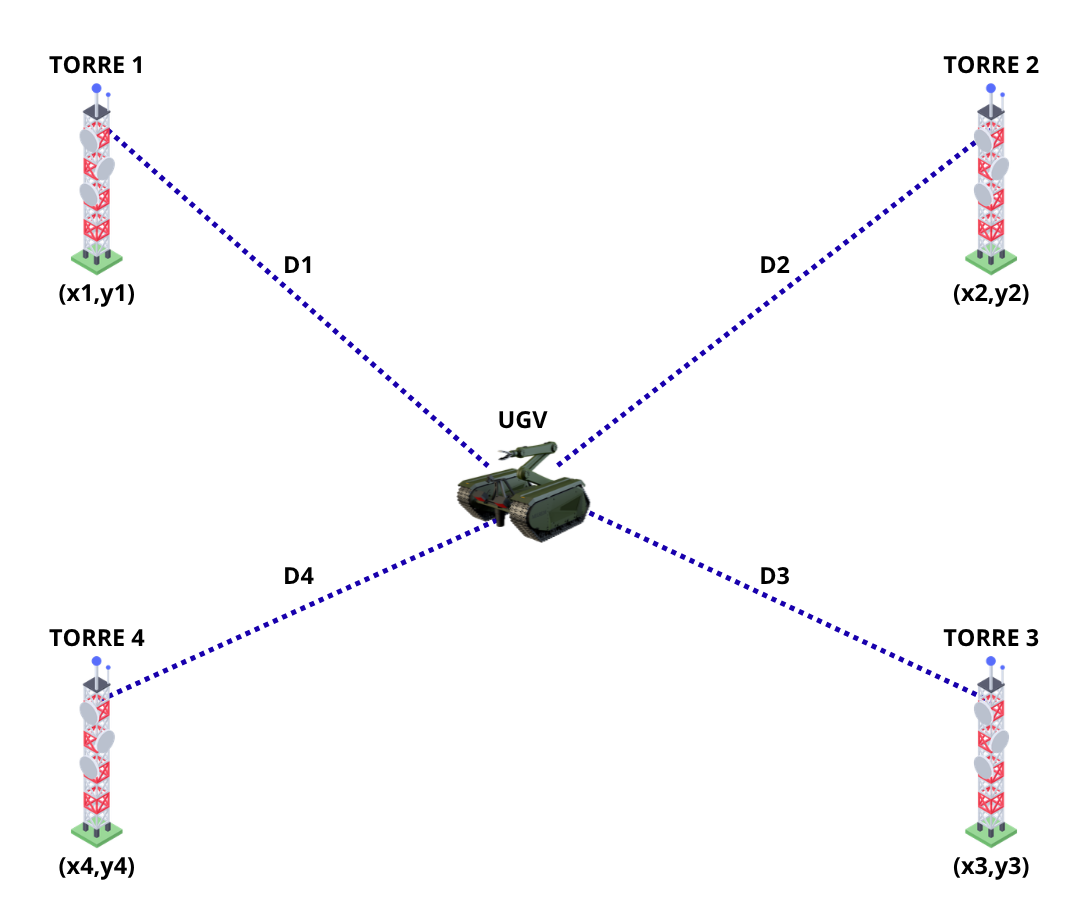
\includegraphics[width=0.5\textwidth]{Figuras/diagrams/MULTILATERAÇÃO.png}
    \caption{Representação geométrica do sistema de posicionamento: o agente móvel no espaço bidimensional e os raios de medição (\textit{range-only}) oriundos das quatro estações base fixas nos vértices da arena.}
    \label{fig:diagrama_multilateracao}
\end{figure}


\subsection{Modelo Cinemático de Processo (Espaço de Estados PVA)}
\label{subsec:pva_model}

Diferentemente de abordagens simplificadas de velocidade constante, o estado do agente móvel no instante discreto $k$ passa a ser representado por um vetor expandido de seis dimensões: $\mathbf{x}_k = [x_k, y_k, v_{x,k}, v_{y,k}, a_{x,k}, a_{y,k}]^T$. Nessa estrutura, $(x_k, y_k)$ correspondem às coordenadas de posição cartesiana, $(v_{x,k}, v_{y,k})$ às componentes da velocidade linear e $(a_{x,k}, a_{y,k})$ às acelerações instantâneas nos eixos $X$ e $Y$, respectivamente.

A dinâmica temporal do sistema sob regime de aceleração constante (CA) é integrada ao longo do intervalo de amostragem $\Delta t$. Essa operação dá origem à matriz de transição de estados $\mathbf{A}_k$ ($6 \times 6$), especificada na Equação (\ref{eq:matriz_A_pva}):

\begin{equation}
    \label{eq:matriz_A_pva}
    \mathbf{A}_k = \begin{bmatrix} 
    1 & 0 & \Delta t & 0 & \frac{\Delta t^2}{2} & 0 \\ 
    0 & 1 & 0 & \Delta t & 0 & \frac{\Delta t^2}{2} \\ 
    0 & 0 & 1 & 0 & \Delta t & 0 \\ 
    0 & 0 & 0 & 1 & 0 & \Delta t \\ 
    0 & 0 & 0 & 0 & 1 & 0 \\ 
    0 & 0 & 0 & 0 & 0 & 1 
    \end{bmatrix}
\end{equation}

Fatores práticos como o escorregamento de rodas, desalinhamentos mecânicos e irregularidades do terreno introduzem erros cumulativos na navegação \cite{thrun2005probabilistic}. Na formulação PVA escolhida, esse comportamento estocástico é transposto para o modelo admitindo que as perturbações ajam de forma independente sobre os componentes de posição, velocidade e aceleração. Essas fontes de incerteza são sintetizadas pela matriz de densidade espectral de potência contínua $\mathbf{Q}_c = \text{diag}(q_1, q_2, q_3, q_4, q_5, q_6)$. 

Ao calcular a discretização analítica desse termo, ponderada pela própria dinâmica veicular no intervalo $\Delta t$, obtém-se uma matriz de covariância discreta $\mathbf{Q}_k$ caracterizada por ser esparsa e simétrica. O perfil estritamente diagonal de $\mathbf{Q}_c$ garante o desacoplamento estocástico entre as dinâmicas dos eixos horizontal ($X$) e vertical ($Y$). Os elementos não nulos associados aos estados do eixo X (índices 0, 2 e 4) são calculados conforme as relações dispostas na Equação (\ref{eq:matriz_Q_pva_x}):

\begin{equation}
    \label{eq:matriz_Q_pva_x}
    \begin{cases}
        Q_{0,0} = q_1\Delta t + q_3\frac{\Delta t^3}{3} + q_5\frac{\Delta t^5}{20} \\
        Q_{0,2} = Q_{2,0} = q_3\frac{\Delta t^2}{2} + q_5\frac{\Delta t^4}{8} \\
        Q_{0,4} = Q_{4,0} = q_5\frac{\Delta t^3}{6} \\
        Q_{2,2} = q_3\Delta t + q_5\frac{\Delta t^3}{3} \\
        Q_{2,4} = Q_{4,2} = q_5\frac{\Delta t^2}{2} \\
        Q_{4,4} = q_5\Delta t
    \end{cases}
\end{equation}

De maneira análoga, os componentes vinculados ao eixo Y (índices 1, 3 e 5) replicam essa mesma estrutura algébrica, utilizando as variâncias espectrais específicas $\{q_2, q_4, q_6\}$ detalhadas na Equação (\ref{eq:matriz_Q_pva_y}):

\begin{equation}
    \label{eq:matriz_Q_pva_y}
    \begin{cases}
        Q_{1,1} = q_2\Delta t + q_4\frac{\Delta t^3}{3} + q_6\frac{\Delta t^5}{20} \\
        Q_{1,3} = Q_{3,1} = q_4\frac{\Delta t^2}{2} + q_6\frac{\Delta t^4}{8} \\
        Q_{1,5} = Q_{5,1} = q_6\frac{\Delta t^3}{6} \\
        Q_{3,3} = q_4\Delta t + q_6\frac{\Delta t^3}{3} \\
        Q_{3,5} = Q_{5,3} = q_6\frac{\Delta t^2}{2} \\
        Q_{5,5} = q_6\Delta t
    \end{cases}
\end{equation}


\subsection{Modelo de Observação e Geometria das Estações Base}
\label{subsec:observation_model}

A partir do arranjo de infraestrutura detalhado na Seção \ref{subsec:problem_description}, o vetor de observações obtido a cada passo amostral é estruturado como $\mathbf{z}_k = [z_{1,k}, z_{2,k}, z_{3,k}, z_{4,k}]^T$. A relação geométrica entre o estado cinemático estimado do robô e a distância escalar real até a $i$-ésima estação fixa é governada por uma função de observação não linear $h_i(\mathbf{x}_k)$, descrita na Equação (\ref{eq:modelo_distancia_nao_linear}):

\begin{equation}
    \label{eq:modelo_distancia_nao_linear}
    h_i(\mathbf{x}_k) = \sqrt{(x_k - X_i)^2 + (y_k - Y_i)^2}
\end{equation}

Como o vetor de estado possui seis dimensões e as leituras dependem estritamente das coordenadas de posição $(x_k, y_k)$, as derivadas parciais da função de medição associadas aos componentes de velocidade e aceleração anulam-se por completo \cite{barshalom2001estimation}. Sob essas condições, a matriz Jacobiana $\mathbf{H}_k$ ($4 \times 6$) avaliada a cada iteração assume o formato estabelecido na Equação (\ref{eq:jacobiano_implementado}):

\begin{equation}
    \label{eq:jacobiano_implementado}
    \mathbf{H}_k = \begin{bmatrix} 
    \frac{x_k - X_1}{h_1(\mathbf{x}_k)} & \frac{y_k - Y_1}{h_1(\mathbf{x}_k)} & 0 & 0 & 0 & 0 \\ 
    \vdots & \vdots & \vdots & \vdots & \vdots & \vdots \\ 
    \frac{x_k - X_4}{h_4(\mathbf{x}_k)} & \frac{y_k - Y_4}{h_4(\mathbf{x}_k)} & 0 & 0 & 0 & 0 
    \end{bmatrix}_{\mathbf{x}_k = \hat{\mathbf{x}}_{k|k-1}}
\end{equation}

Para concluir a modelagem matemática do sensor, a matriz de covariância do ruído de medição é definida como $\mathbf{R}_k = \text{diag}(\sigma_1^2, \sigma_2^2, \sigma_3^2, \sigma_4^2)$, em que cada termo diagonal reflete a variância do erro instrumental intrínseco de sua respectiva âncora de leitura.


\subsection{Cenário de Desafio: Modelagem de Oclusão Temporal}
\label{subsec:occlusion_challenge}

Para avaliar os limites do estimador e a utilidade prática da região de interesse (ROI) dinâmica e do teste NIS, projetou-se uma janela de oclusão severa no ambiente de simulação. Dentro de um intervalo cronometrado $t \in [t_{\text{start}}, t_{\text{end}}]$, as leituras vindas das quatro estações base são intencionalmente suprimidas ($\mathbf{z}_{i,k} \to \emptyset$).

Esse bloqueio — cujo comportamento é ilustrado na Figura \ref{fig:comportamento_elipses} — força o algoritmo a depender apenas das projeções geradas pela matriz de transição PVA (\ref{eq:matriz_A_pva}). Sob condições normais de operação com o filtro atualizando as medições, a elipse mantém-se estável e restrita (Figura \ref{fig:elipse_estavel}). Contudo, sem o suporte das correções trazidas pelos sensores durante a oclusão, as incertezas de aceleração modeladas em $\mathbf{Q}_k$ acumulam-se rapidamente. O resultado direto é uma expansão geométrica acentuada na matriz de covariância predita ($\mathbf{P}_{k|k-1}$), que se traduz no alargamento progressivo da elipse de confiança (ROI) ao longo do deslocamento do robô, variando conforme a trajetória realizada (Figuras \ref{fig:elipse_crescente_1} e \ref{fig:elipse_crescente_2}).


\begin{figure*}[t!]
    \centering
    
    % Subfigura A: Filtro atualizando / Comportamento estável
    \begin{subfigure}[b]{0.32\textwidth}
        \centering
        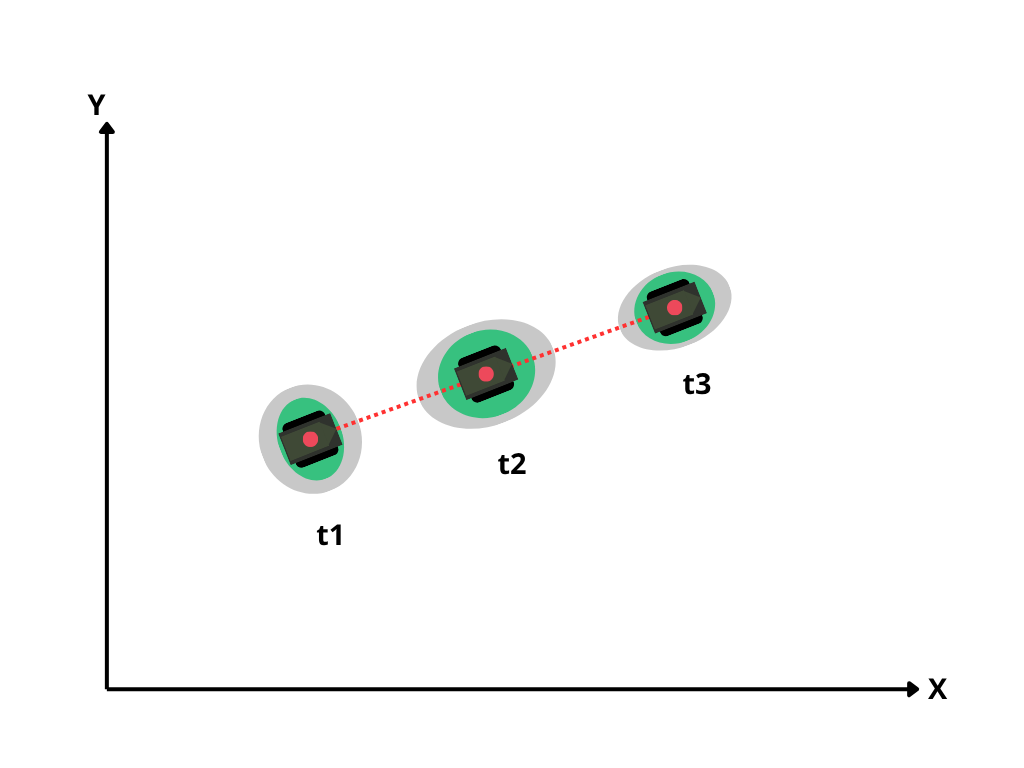
\includegraphics[width=\linewidth]{Figuras/diagrams/PREVISAO.png}
        \caption{Operação nominal: predição e atualização.}
        \label{fig:elipse_estavel}
    \end{subfigure}
    \hfill
    % Subfigura B: Crescimento na trajetória 1
    \begin{subfigure}[b]{0.32\textwidth}
        \centering
        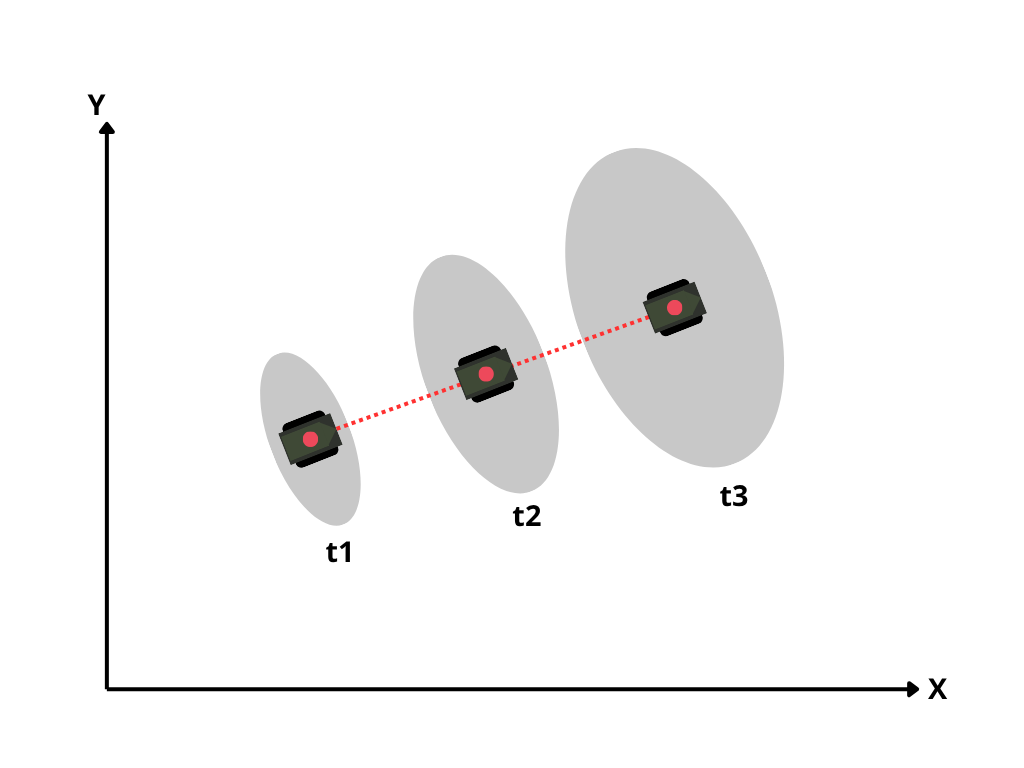
\includegraphics[width=\linewidth]{Figuras/diagrams/OCLUSAO.png}
        \caption{Oclusão: trajetória 1 (predição pura).}
        \label{fig:elipse_crescente_1}
    \end{subfigure}
    \hfill
    % Subfigura C: Crescimento na trajetória 2
    \begin{subfigure}[b]{0.32\textwidth}
        \centering
        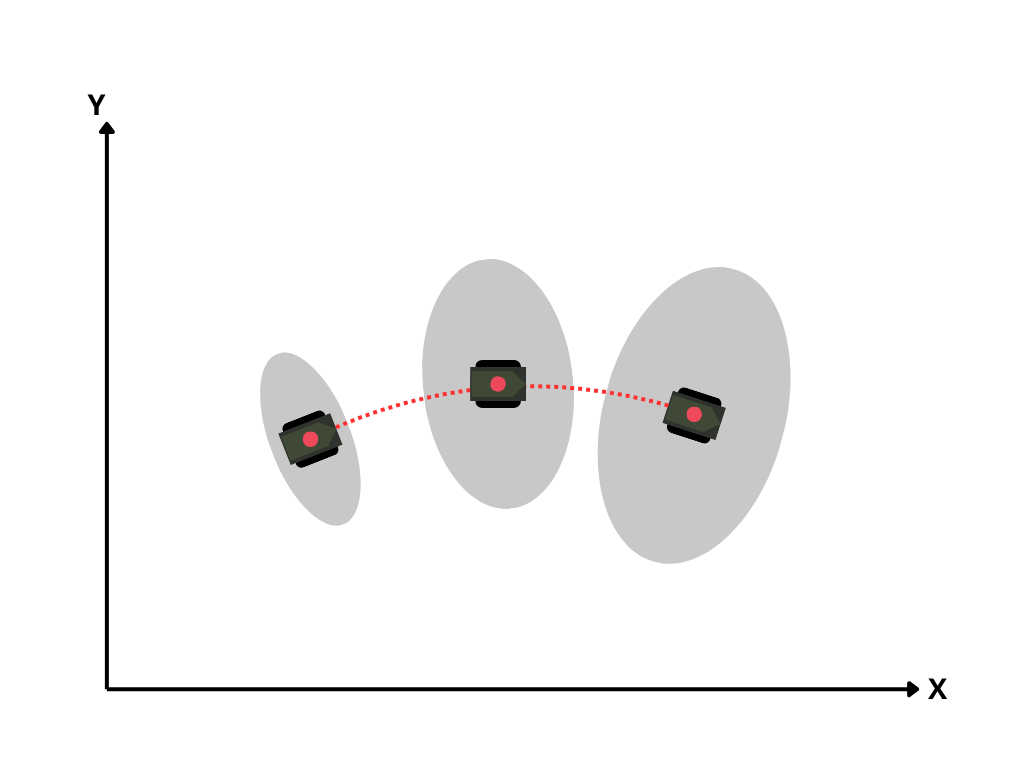
\includegraphics[width=\linewidth]{Figuras/diagrams/OCLUSAO2.png}
        \caption{Oclusão: trajetória 2 (predição pura).}
        \label{fig:elipse_crescente_2}
    \end{subfigure}

    \caption{Representação visual da incerteza do EKF (ROI dinâmica): a elipse em cinza denota a incerteza predita ($\mathbf{P}_{k|k-1}$), enquanto a elipse em verde representa a incerteza atualizada após a correção ($\mathbf{P}_{k|k}$). (a) Regime de operação estável sob observações contínuas; (b) e (c) expansão da incerteza e degradação da precisão decorrentes da supressão das medições (oclusão temporal) em distintos perfis de trajetória.}
    \label{fig:comportamento_elipses}
\end{figure*}

% Capítulo 4: Metodologia
% ============================================================
% CAPÍTULO 4: METODOLOGIA E EXPERIMENTAÇÃO
% ============================================================
\section{Metodologia e Experimentação}
\label{sec:methodology}

Este capítulo detalha a metodologia utilizada para avaliar o desempenho, a sensibilidade e a robustez à oclusão do estimador proposto. A apresentação segue a ordem lógica dos experimentos: inicialmente, descreve-se a geração cinemática das trajetórias de referência. Em seguida, detalham-se os cenários de teste e a modelagem do filtro. Por fim, definem-se as métricas estatísticas aplicadas na avaliação do Filtro de Kalman Estendido (EKF) sob diferentes parametrizações.

\subsection{Síntese Cinemática das Trajetórias de Referência}
\label{subsec:trajectory_generation}

Para que a precisão do Filtro de Kalman Estendido (EKF) possa ser avaliada, é indispensável compará-lo a um referencial absoluto e livre de ruídos, o \textit{Ground Truth}. Nessa etapa, o simulador atua como um gerador de gabaritos: ele calcula a física exata do alvo para cada instante discreto $k$ e armazena essas informações no vetor de estado $\mathbf{x}_k = [p_{x}, p_{y}, v_{x}, v_{y}, a_{x}, a_{y}]^T$, que engloba as posições, velocidades e acelerações reais nos eixos ortogonais.

Como um alvo em uma aplicação real pode apresentar desde um trajeto altamente previsível até manobras bruscas, o simulador foi projetado para testar os limites do estimador utilizando duas abordagens distintas de movimento:
\begin{itemize}
    \item \textbf{Curvas paramétricas analíticas (Determinísticas):} Simulam cenários onde o alvo obedece a regras geométricas bem definidas e contínuas. Servem para testar o filtro sob dinâmicas estáveis e previsíveis.
    \item \textbf{Modelos numéricos comportamentais (Estocásticos):} Inserem aleatoriedade na navegação do alvo. Servem para testar a capacidade de adaptação do EKF quando o objeto realiza trajetórias erráticas ou mudanças repentinas de direção.
\end{itemize}

O conjunto completo dessas trajetórias, abrangendo todos os perfis cinemáticos abordados nos testes, pode ser visualizado na Figura \ref{fig:trajetorias_simulacao}.

\subsubsection{Geração de Curvas Paramétricas e Analíticas}

Para os testes com movimentos contínuos e regulares, as posições do alvo no simulador são ditadas por funções trigonométricas e hiperbólicas dependentes do tempo. Um cuidado fundamental nessa etapa foi evitar o cálculo numérico das derivadas. Para garantir que o \textit{Ground Truth} seja matematicamente exemplar e livre de erros de discretização, a velocidade e a aceleração do alvo são extraídas a partir da diferenciação analítica exata das equações de posição, conforme detalha o Algoritmo \ref{alg:traj_analitica}.

\begin{algorithm}[h]
\caption{Geração de Trajetórias Paramétricas Analíticas}
\label{alg:traj_analitica}
\begin{algorithmic}[1]
\Require Tempo contínuo $t_k = k \Delta t$, Parâmetros geométricos (Amplitude $A$, Frequência $\omega$)
\For{cada instante $k$}
    \If{Perfil = Circular}
        \State $\mathbf{p}_k \gets [c_x + R\cos(\omega t_k), \; c_y + R\sin(\omega t_k)]^T$
    \ElsIf{Perfil = Mudança de Faixa (Tanh)}
        \State $\mathbf{p}_k \gets [v_x t_k, \; c_y + A\tanh(S \cdot t_k)]^T$
    \ElsIf{Perfil = Lemniscata}
        \State $\mathbf{p}_k \gets [c_x + A\sin(\omega t_k), \; c_y + \frac{A}{2}\sin(2\omega t_k)]^T$
    \EndIf
    
    \State $\mathbf{v}_k \gets \frac{d}{dt}\mathbf{p}_k$
    \State $\mathbf{a}_k \gets \frac{d}{dt}\mathbf{v}_k$
    \State $\mathbf{x}_k \gets [\mathbf{p}_k^T, \mathbf{v}_k^T, \mathbf{a}_k^T]^T$
\EndFor
\Ensure Sequência de estados reais $\mathbf{x}_{1:N}$
\end{algorithmic}
\end{algorithm}

As trajetórias com quinas, como o percurso quadrado, obedecem a esse mesmo rigor determinístico. A única diferença é que a modelagem utiliza segmentos de reta conectados para formar as arestas, aplicando-se uma restrição geométrica de fechamento para garantir que o alvo retorne exatamente à coordenada onde iniciou o percurso.

\subsubsection{Geração de Navegação Aleatória e Oclusões}

\begin{figure*}[t!]
    \centering
    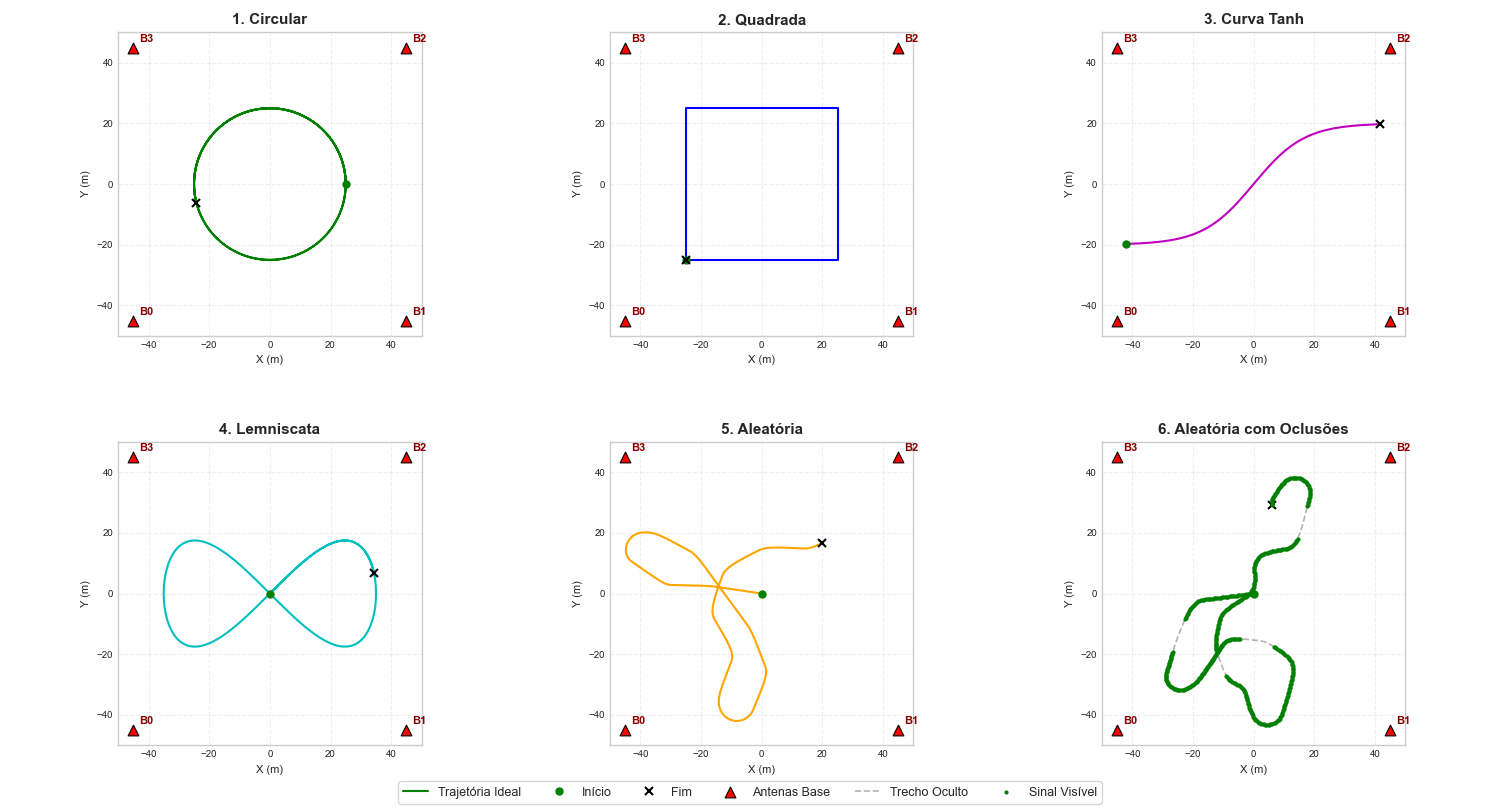
\includegraphics[width=\textwidth]{Figuras/diagrams/trajetorias.png}
    
    \caption{Visualização bidimensional das trajetórias de referência (\textit{Ground Truth}) geradas pelo motor de simulação para a avaliação do estimador sob diferentes perfis cinemáticos.}
    \label{fig:trajetorias_simulacao}
\end{figure*}

Para aproximar a simulação do comportamento estocástico de um alvo real, desenvolveu-se um algoritmo de navegação aleatória. O agente (UGV - Unmanned Ground Vehicle) move-se em linha reta por distâncias mínimas antes de realizar deflexões suaves. Se o robô atinge os limites da arena (raio superior a $35$ metros), um mecanismo de evasão direciona o movimento de volta ao centro, mantendo o robô na área útil.

Como as mudanças de direção são aleatórias, a aceleração de referência é calculada por diferenciação numérica discreta, conforme estruturado no Algoritmo \ref{alg:traj_aleatoria}.

\begin{algorithm}[h]
\caption{Geração de Navegação Dinâmica Aleatória}
\label{alg:traj_aleatoria}
\begin{algorithmic}[1]
\Require Vetor posição central $\mathbf{p}_c$, Limite da arena $R_{\max}$, Ruído cinemático $w$
\For{cada instante $k$}
    \If{Distância percorrida $> D_{\min}$}
        \If{$\|\mathbf{p}_{k-1} - \mathbf{p}_c\| > R_{\max}$}
            \State $\theta_{\text{alvo}} \gets$ Ângulo forçado em direção a $\mathbf{p}_c$
        \Else
            \State $\theta_{\text{alvo}} \gets \theta_{k-1} + \mathcal{U}(-\frac{\pi}{3}, \frac{\pi}{3})$
        \EndIf
        \State $v_{\text{alvo}} \gets v_{\text{base}} + \mathcal{U}(-w, w)$
    \EndIf
    
    \State $\theta_k \gets \text{SuavizarTransição}(\theta_{k-1}, \theta_{\text{alvo}})$
    \State $v_k \gets \text{SuavizarTransição}(v_{k-1}, v_{\text{alvo}})$
    
    \State $\mathbf{v}_k \gets [v_k\cos(\theta_k), \; v_k\sin(\theta_k)]^T$
    \State $\mathbf{p}_k \gets \mathbf{p}_{k-1} + \mathbf{v}_k \Delta t$
    \State $\mathbf{a}_k \gets (\mathbf{v}_k - \mathbf{v}_{k-1}) / \Delta t$
\EndFor

\Statex \textbf{Configuração Especial para Oclusão Cíclica:}
\If{Modo Oclusão}
    \State Emite uma máscara binária atribuindo valor \textit{Falso} (Oculto) no segmento temporal central de 4 blocos.
\EndIf
\end{algorithmic}
\end{algorithm}

\subsection{Cenários de Simulação e Estratégia de Sintonia}
\label{subsec:cenarios_sintonia}

Para avaliar o estimador na prática, a campanha de testes foi dividida em \textbf{6 cenários cinemáticos} (ilustrados na Figura \ref{fig:trajetorias_simulacao}), abrangendo diferentes perfis de aceleração e condições de oclusão. Além do movimento do alvo, o comportamento do EKF depende diretamente das suas matrizes de covariância ($\mathbf{Q}_k$ para o processo e $\mathbf{R}_k$ para a medição). Para testar a robustez e a sensibilidade do algoritmo a esses parâmetros, cada cenário foi avaliado sob \textbf{duas condições de sintonia distintas}:

\begin{enumerate}
    \item \textbf{Situação Sintonizada (Filtro Calibrado):} Representa a condição de funcionamento ideal do rastreador. Os valores das matrizes foram ajustados de forma empírica, baseando-se nas propriedades do ambiente e refinados por tentativa e erro até que o filtro apresentasse o melhor desempenho. A matriz de medição foi definida como $\mathbf{R} = 0,09\mathbf{I}_4$ (quadrado do desvio padrão do ruído das torres, $\sigma = 0,30$ m), enquanto a matriz de processo foi fixada em $\mathbf{Q} = 0,64\mathbf{I}_6$ ($0,8^2$), assumindo estatisticamente as incertezas de modelagem do movimento. O critério de sucesso foi a minimização do erro de posição aliada a elipses de confiança visualmente e estatisticamente coerentes com a trajetória real.
    
    \item \textbf{Situação Não Sintonizada (Filtro Descalibrado):} Representa falhas na configuração do projeto. Nessa etapa, os valores das matrizes foram intencionalmente alterados por superestimação (Sup.) ou subestimação (Sub.). O objetivo de impor essas condições anormais é avaliar a sensibilidade do estimador, demonstrar o impacto do desalinhamento de covariâncias no erro adaptativo e comprovar a importância de uma sintonia rigorosa.
\end{enumerate}

A Tabela \ref{tab:parametros_simulacao} consolida todas as variáveis utilizadas nos testes: a configuração de movimento do alvo, o nível de ruído físico ($\sigma$) simulado nos sensores e os valores numéricos utilizados para sintonizar (ou descalibrar) o EKF em cada um dos seis cenários.

\begin{table*}[t!]
\centering
\caption{Parâmetros de Configuração Cinemática e Sintonia das Matrizes (Mundo Simulado vs. Estimador EKF)}
\label{tab:parametros_simulacao}
\small
\begin{tabular}{lcccccc}
\hline \hline
\textbf{Parâmetro} & \textbf{Cenário 1} & \textbf{Cenário 2} & \textbf{Cenário 3} & \textbf{Cenário 4} & \textbf{Cenário 5} & \textbf{Cenário 6} \\ \hline
\textbf{Perfil} & Circular & Quadrada & Tanh & Lemniscata & Nav. Aleatória & Oclusão Cíclica \\ \addlinespace[1mm]

\textbf{Movimento} & \begin{tabular}{@{}c@{}}$v = 10,0$ m/s \\ $r = 30,0$ m\end{tabular} & \begin{tabular}{@{}c@{}}$v = 10$ m/s \\ $L = 40,0$ m\end{tabular} & \begin{tabular}{@{}c@{}}$A_y = 20,0$ m \\ $v= 10,0$ m/s\end{tabular} & \begin{tabular}{@{}c@{}}$v = 10,0$ m/s \\ $A = 35,0$ m\end{tabular} & \begin{tabular}{@{}c@{}}$v_0 = 8,0$ m/s \\  $\epsilon_v = 0,5$ m/s\end{tabular} & \begin{tabular}{@{}c@{}}$v = 5,0$ m/s \\ 30 fr/oclusão \end{tabular} \\ \addlinespace[2mm]

\multicolumn{7}{c}{\cellcolor{gray!20}\textbf{Variáveis do Ambiente Simulado (Adição de Ruído Físico)}} \\ \addlinespace[1mm]
\textbf{Posição das Torres} & \multicolumn{6}{c}{$B_1[10,10]$; $B_2[190,10]$; $B_3[190,130]$; $B_4[10,130]$} \\ \addlinespace[1mm]
\textbf{Tempo de Simulação} & \multicolumn{6}{c}{40 s} \\ \addlinespace[1mm]
\textbf{Taxa de Quadros (FPS)} & \multicolumn{6}{c}{30} \\ \addlinespace[1mm]
\textbf{Semente Aleatória (\textit{Seed})} & \multicolumn{6}{c}{42} \\ \addlinespace[1mm]
\textbf{Ruído nas Torres ($\sigma$)} & $0,30$ m & $0,30$ m & $0,30$ m & $0,30$ m & $0,30$ m & $0,30$ m \\ \addlinespace[2mm]

\multicolumn{7}{c}{\cellcolor{gray!20}\textbf{Sintonia do EKF: Condição Sintonizada}} \\ \addlinespace[1mm]
\textbf{Matriz Medição $\mathbf{R}_{4\times4}$} & $0,09 \mathbf{I}_{4}$ & $0,09 \mathbf{I}_{4}$ & $0,09 \mathbf{I}_{4}$ & $0,09 \mathbf{I}_{4}$ & $0,09 \mathbf{I}_{4}$ & $0,09 \mathbf{I}_{4}$ \\ \addlinespace[1mm]
\textbf{Matriz Processo $\mathbf{Q}_{6\times6}$} & $0.64\mathbf{I}_{6}$ & $0.64 \mathbf{I}_{6}$ & $0.64 \mathbf{I}_{6}$ & $0.64 \mathbf{I}_{6}$ & $0.64 \mathbf{I}_{6}$ & $0.64 \mathbf{I}_{6}$ \\ \addlinespace[2mm]

\multicolumn{7}{c}{\cellcolor{gray!20}\textbf{Sintonia do EKF: Condição Não Sintonizada}} \\ \addlinespace[1mm]
\textbf{Matriz Medição $\mathbf{R}_{4\times4}$} & \begin{tabular}{@{}c@{}}$0,1 \mathbf{I}_{4}$ \\ (Sup.)\end{tabular} & \begin{tabular}{@{}c@{}}$0,1 \mathbf{I}_{4}$ \\ (Sup.)\end{tabular} & \begin{tabular}{@{}c@{}}$0,01 \mathbf{I}_{4}$ \\ (Sub.)\end{tabular} & $0,09 \mathbf{I}_{4}$ & \begin{tabular}{@{}c@{}}$0,01 \mathbf{I}_{4}$ \\ (Sub.)\end{tabular} & \begin{tabular}{@{}c@{}}$0,01 \mathbf{I}_{4}$ \\ (Sub.)\end{tabular} \\ \addlinespace[1mm]
\textbf{Matriz Processo $\mathbf{Q}_{6\times6}$} & \begin{tabular}{@{}c@{}}$0,01 \mathbf{I}_{6}$ \\ (Sub.)\end{tabular} & \begin{tabular}{@{}c@{}}$0,01 \mathbf{I}_{6}$ \\ (Sub.)\end{tabular} & \begin{tabular}{@{}c@{}}$0,5 \mathbf{I}_{6}$ \\ (Sub.)\end{tabular} & \begin{tabular}{@{}c@{}}$0,3 \mathbf{I}_{6}$ \\ (Sub.)\end{tabular} & \begin{tabular}{@{}c@{}}$0,5 \mathbf{I}_{6}$ \\ (Sub.)\end{tabular} & \begin{tabular}{@{}c@{}}$0,05 \mathbf{I}_{6}$ \\ (Sub.)\end{tabular} \\ \hline \hline

\multicolumn{7}{p{16cm}}{\scriptsize \textit{Nota:} $\mathbf{I}_{n}$ representa a matriz identidade de dimensão $n \times n$, denotando configurações diagonais. A matriz $\mathbf{R}$ apresenta um superdimensionamento conservador intencional ($0,9 \mathbf{I}_{4}$), não refletindo estritamente a variância do ruído injetado ($\sigma^2$). No Cenário 4 (Não Sintonizado), $\mathbf{R}$ foi propositalmente mantido inalterado para isolar e avaliar exclusivamente o efeito da subestimação de $\mathbf{Q}$. (Sup.) = Descalibração por Superestimação; (Sub.) = Descalibração por Subestimação.}
\end{tabular}
\end{table*}

\subsection{Configuração do Estimador e Modelagem do Ruído}
\label{subsec:estimator_config}

O objetivo do filtro é estimar o estado completo do alvo (o vetor PVA $\mathbf{x}_k$, detalhado na Seção \ref{sec:problem_formulation}). Para alimentar o algoritmo, o sistema mede a distância do robô até quatro estações rádio-base fixadas nos cantos da arena.

Como nenhum sensor no mundo real é perfeito, o simulador precisa "sujar" as medidas ideais do \textit{Ground Truth}. Para imitar a imprecisão real, o sistema injeta um erro aleatório em cada canal: soma-se à distância exata um ruído gaussiano branco de média zero e desvio padrão $\sigma$ (valores indicados na Tabela \ref{tab:parametros_simulacao}). 

Isso resulta no vetor de observação $\mathbf{z}_k = [z_{1,k}, z_{2,k}, z_{3,k}, z_{4,k}]^T$, que contém as quatro distâncias ruidosas que o EKF efetivamente recebe como entrada, conforme a Equação (\ref{eq:ruido_interface}):
\begin{equation}
    z_{i,k} = \| \mathbf{p}_k - \mathbf{p}_{i} \| + v_{i,k}, \quad v_{i,k} \sim \mathcal{N}(0, \sigma^2) \quad \forall \quad i = 1, \dots, 4
    \label{eq:ruido_interface}
\end{equation}

É importante destacar que o EKF trabalha diretamente com essas distâncias puras na sua forma não-linear ($\mathbf{z}_k$). No entanto, para que possamos desenhar a posição lida pelos sensores na interface gráfica do simulador, o sistema realiza um cálculo paralelo. Ele pega essas quatro distâncias com ruído e aplica um algoritmo numérico de multilateração por Mínimos Quadrados para estimar uma coordenada cartesiana $\mathbf{m}_k = [m_{x,k}, m_{y,k}]^T$. Essa coordenada 2D serve estritamente como apoio visual para a tela e para a validação externa, não interferindo nas contas do Filtro de Kalman.

\subsection{Ambiente Computacional e Infraestrutura de Simulação}
\label{subsec:software_environment}

\begin{figure}[htbp]
    \centering   
    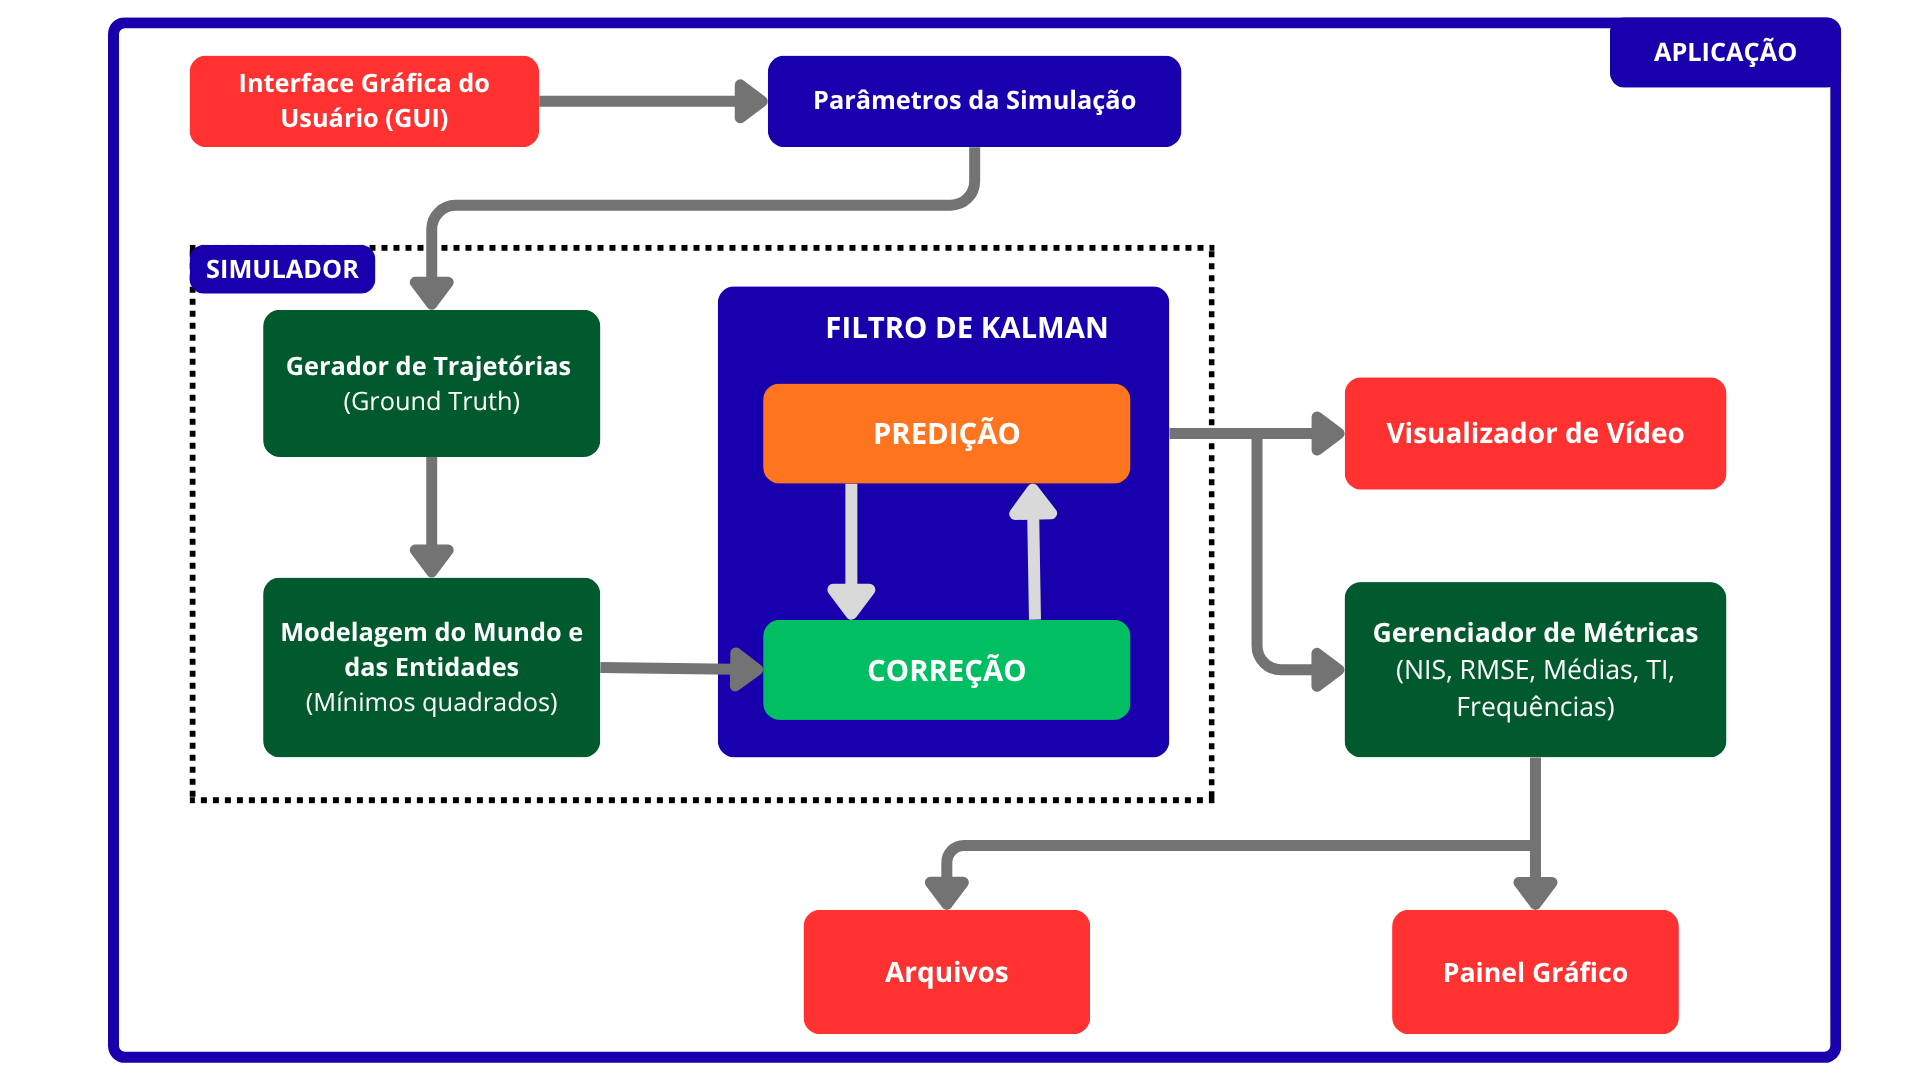
\includegraphics[width=\columnwidth]{Figuras/diagrams/ARQUITETURA.png}
    \caption{Diagrama da arquitetura de software da aplicação de simulação, destacando o fluxo de dados entre o gerador de trajetórias, o estimador de estados e a camada de aplicação.}
    \label{fig:arquitetura_software}
\end{figure}

Para automatizar a execução dos cenários e garantir a reprodutibilidade dos dados, o simulador foi desenvolvido em \textit{Python} (versão 3.10) utilizando uma arquitetura modular, conforme ilustrado na Figura \ref{fig:arquitetura_software}. O processamento matricial e a computação vetorizada do EKF foram implementados com a biblioteca \textit{NumPy}.

Conforme detalhado no diagrama, a arquitetura divide-se logicamente entre o núcleo de simulação e a camada de aplicação. O fluxo de execução inicia-se na Interface Gráfica do Usuário (GUI), onde são definidos os parâmetros iniciais, incluindo a sintonia empírica das matrizes de covariância de processo ($\mathbf{Q}_k$) e de ruído de medição ($\mathbf{R}_k$). Esses parâmetros alimentam o bloco \textit{Simulador}, onde o \textit{Gerador de Trajetórias} estabelece a cinemática real do alvo (\textit{ground truth}). 

Para avaliar adequadamente a capacidade de estimação do filtro, a trajetória exata é ramificada para dois destinos: o \textit{Gerenciador de Métricas} (servindo como base de comparação para o cálculo de erros) e a \textit{Modelagem do Mundo e das Entidades}. Este último atua como o simulador do sistema de localização, convertendo as posições reais em distâncias ruidosas relativas a quatro torres (multilateração). Essa pseudo-observação ruidosa alimenta, então, a etapa de \textit{Correção} do Filtro de Kalman, que trabalha em malha fechada com a \textit{Predição} estocástica.

A GUI, construída nativamente com a biblioteca \textit{Tkinter}, não se limita à parametrização, atuando também na camada de \textit{Aplicação}. Ela integra o \textit{Visualizador de Vídeo} — que renderiza instantaneamente o vetor de observações e a elipse de incerteza da região de interesse (ROI) — e os painéis do \textit{Gerenciador de Métricas}, que acompanham as estatísticas de NIS e RMSE. Apesar dessa integração visual para inspeção qualitativa, o núcleo numérico do simulador opera de forma independente, garantindo que as campanhas de teste em lote e a geração de arquivos de log ocorram de forma assíncrona e automatizada.

\subsection{Métodos de Avaliação e Consistência}
\label{subsec:metricas_metodologia}

O desempenho do EKF é avaliado pela sua precisão espacial e consistência estatística. A acurácia geométrica é quantificada pela Raiz do Erro Quadrático Médio ($\text{RMSE}$), calculada de forma independente para os eixos $X$ e $Y$ ao comparar as estimativas \textit{a posteriori} $(\hat{x}_{k|k}, \hat{y}_{k|k})$ com o \textit{Ground Truth}. O erro médio com sinal ($\text{ME}$) também é monitorado para identificar eventuais vieses sistemáticos no rastreamento.

Embora a análise espacial meça a exatidão geométrica, ela não garante o equilíbrio estatístico do estimador. Para a validação formal de consistência, utiliza-se o \textit{Normalized Innovation Squared} ($\text{NIS}$). O teste do $\text{NIS}$ avalia se a magnitude dos resíduos de inovação é coerente com a incerteza teórica parametrizada nas matrizes de covariância $\mathbf{Q}_k$ e $\mathbf{R}_k$ \cite{barshalom2001estimation}.

\subsubsection{Validação da Crença do Estimador (\textit{Inlier Rate})}
\label{subsubsec:validacao_inliers}

Como métrica complementar em ambiente de simulação, a convergência da crença (\textit{belief}) do filtro é avaliada graficamente pela taxa de \textit{inliers}. Por depender do \textit{Ground Truth}, essa abordagem restringe-se à calibração e análise do comportamento do modelo frente a dados sintéticos controlados.

Baseando-se no conceito de elipsoide de erro \cite{thrun2005probabilistic}, quantifica-se a proporção de frames em que o estado real ($x_{GT}, y_{GT}$) permanece contido na fronteira de incerteza do filtro. A validação baseia-se na distância de Mahalanobis aplicada sobre a submatriz de covariância de posição \textit{a posteriori} $\mathbf{P}_{\text{pos}} = \mathbf{P}_{k|k}^{(1:2, 1:2)}$. Definindo o vetor de erro real como $\tilde{\mathbf{p}}_k = [x_{GT,k} - \hat{x}_{k|k}, \; y_{GT,k} - \hat{y}_{k|k}]^T$, o estado é classificado como um \textit{inlier} se atender à restrição:

\begin{equation}
    \tilde{\mathbf{p}}_k^T \left( \mathbf{P}_{\text{pos}} \right)^{-1} \tilde{\mathbf{p}}_k \le M
    \label{eq:condicao_inlier_quadratica}
\end{equation}
em que $M$ é o valor crítico da distribuição Qui-Quadrado ($\chi^2$) bicaudal com 2 graus de liberdade para o nível de significância adotado.

Para a renderização em tempo real na interface gráfica, a elipse é aproximada por uma janela delimitadora (\textit{bounding box}) baseada no critério $3\sigma$. Os desvios-padrão marginais teóricos são dados por:

\begin{equation}
    \sigma_{x, \text{filt}} = \sqrt{\max(10^{-6}, P_{k|k}^{(1,1)})}
    \label{eq:sigma_x}
\end{equation}
\begin{equation}
    \sigma_{y, \text{filt}} = \sqrt{\max(10^{-6}, P_{k|k}^{(2,2)})}
    \label{eq:sigma_y}
\end{equation}

Os limites semi-eixais da janela visual ($L_x, L_y$) incorporam uma constante de salvaguarda inferior $\tau_{\min}$ para evitar o colapso da caixa em cenários de incerteza nula ou falhas de inicialização:

\begin{equation}
    L_x = \max(\tau_{\min}, 3\sigma_{x,\text{filt}})
    \label{eq:Lx}
\end{equation}
\begin{equation}
    L_y = \max(\tau_{\min}, 3\sigma_{y,\text{filt}})
    \label{eq:Ly}
\end{equation}

A Figura \ref{fig:validacao_inliers} ilustra a correlação espacial entre a elipse probabilística (Equação \ref{eq:condicao_inlier_quadratica}) e a janela ortogonal de renderização (Equações \ref{eq:Lx} e \ref{eq:Ly}), permitindo aferir qualitativamente se a dispersão das estimativas é coerente com a evolução da matriz $\mathbf{P}$.

\subsubsection{Análise de Estabilidade Estatística via Limites de Confiança do NIS}
\label{subsubsec:limites_nis}

Enquanto a taxa de \textit{inliers} atua como um validador visual externo restrito à simulação, o $\text{NIS}$ avalia a estabilidade matemática de forma independente do \textit{Ground Truth}, refletindo a operação real do algoritmo. O teste de hipóteses é governado por um intervalo de confiança bicaudal de 95\%, cujos graus de liberdade ($DOF$) dependem do número de torres de recepção ativas na multilateração a cada passo de tempo $k$.

Para um cenário padrão com 4 graus de liberdade (4 DOF), os limites críticos da tabela $\chi^2$ são $\chi^2_{0.025, 4} = 0{,}484$ (inferior) e $\chi^2_{0.975, 4} = 11{,}143$ (superior). O histórico do $\text{NIS}$ permite classificar o comportamento dinâmico do EKF em três regimes:

\begin{itemize}
    \item \textbf{Filtro Consistente:} O $\text{NIS}$ oscila predominantemente dentro dos limites calculados. Espera-se que aproximadamente 95\% das amostras temporais residam nessa faixa, validando a representação correta da própria incerteza do filtro.
    \item \textbf{Filtro Otimista (Subestimação do Erro):} O $\text{NIS}$ ultrapassa repetidamente o limite superior. Isso indica que os resíduos reais são significativamente maiores do que a covariância calculada em $\mathbf{P}$, sinalizando que o filtro confia excessivamente no modelo preditivo em detrimento das medições, o que gera risco de divergência.
    \item \textbf{Filtro Pessimista (Superestimação do Erro):} O $\text{NIS}$ permanece abaixo do limite inferior. Nesse estado, a matriz de covariância cresce de forma desproporcional aos resíduos de inovação. O filtro torna-se excessivamente conservador e lento para responder a variações dinâmicas do alvo.
\end{itemize}

\begin{figure}[htbp]
    \centering
    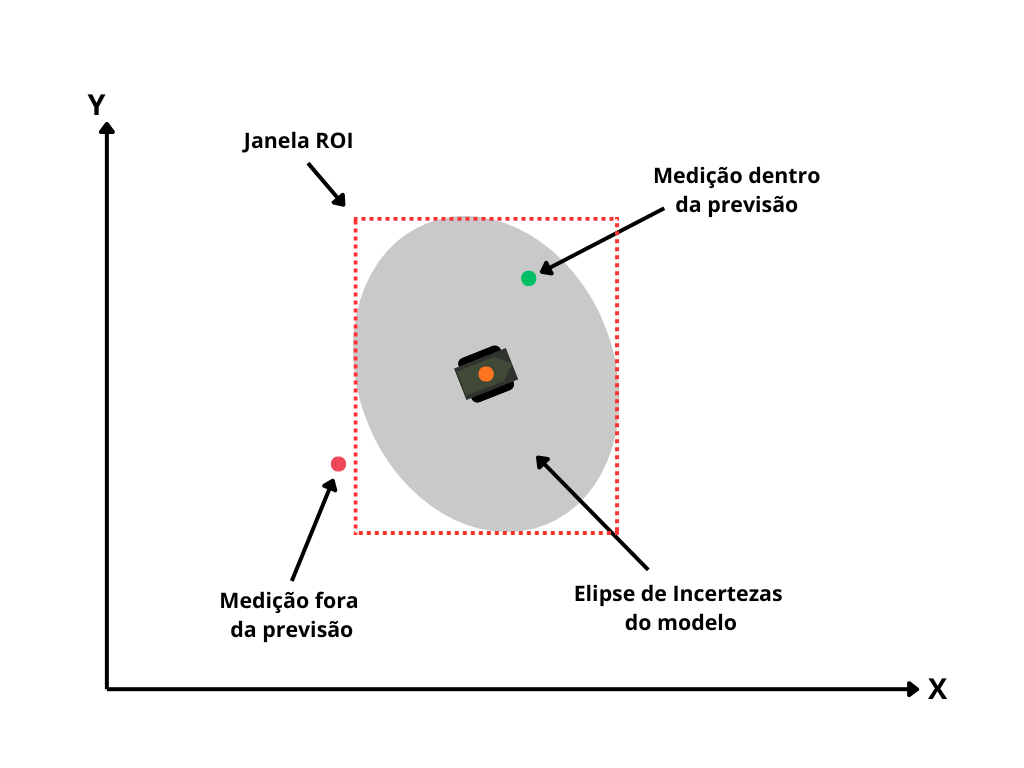
\includegraphics[width=\columnwidth]{Figuras/diagrams/GATTING.png}
    \caption{Representação da métrica de \textit{inliers}. A elipse valida estatisticamente a convergência frente ao Ground Truth, enquanto a janela retangular delimita a incerteza para fins de visualização na GUI.}
    \label{fig:validacao_inliers}
\end{figure}

% Capítulo 5: Resultados
% ============================================================
% CAPÍTULO 5: RESULTADOS E DISCUSSÃO
% ============================================================

\section{Resultados e Discussão}
\label{sec:results}

Este capítulo detalha a avaliação experimental do Filtro de Kalman Estendido (EKF) ao longo dos seis cenários de navegação propostos na Seção \ref{sec:methodology}. A análise fundamenta-se em métricas de acurácia posicional (RMSE e Erro Máximo), consistência estatística (NIS) e validação espacial (Taxa de \textit{Inliers}). Para avaliar a sensibilidade do algoritmo, os ensaios comparam o EKF com matrizes calibradas em contraponto a uma configuração intencionalmente descalibrada. A Tabela \ref{tab:resumo_metricas_dividida_nomes} consolida os indicadores quantitativos obtidos na simulação.

Devido a restrições de formatação, as composições gráficas completas (painéis comparativos de todas as trajetórias estimadas e históricos da métrica NIS para os seis cenários) foram alocadas no \textbf{Apêndice \ref{app:graficos_completos}}. Além disso, o código-fonte do simulador, os dados brutos e as imagens em alta resolução estão publicamente disponíveis no repositório do projeto no GitHub\footnote{Disponível em: \url{https://github.com/SauloJose/PASKalmanTraj} - Acesso em: 22 jun. 2026.}.

% ============================================================
% TABELA DE RESULTADOS 
% ============================================================

\begin{table*}[t!]
\centering
\caption{Resumo das Métricas de Desempenho do EKF (Condição Sintonizada vs. Não Sintonizada)}
\label{tab:resumo_metricas_dividida_nomes}
\small
\begin{tabular}{l *{8}{S[table-format=3.2]}}
\hline \hline
\textbf{Cenário} & {$RMSE_x$ [m]} & {$RMSE_y$ [m]} & {$E_{\max}$ [m]} & {$\mu_x$ [m]} & {$\overline{NIS}$} & {$NIS \in \text{IC}$ [\%]} & {TD [\%]} & {TI [\%]} \\ \hline
\addlinespace[1mm]
\multicolumn{9}{c}{\textbf{CONDIÇÃO SINTONIZADA (Q = 0,64$\mathbf{I_6}$; R = 0,09$\mathbf{I_4}$)}} \\ \hline
\addlinespace[1mm]
\textbf{Cenário 1} & 0,11 & 0,16 & 0,64 & +0,01 & 3,39 & 96,33 & 100,00 & 100,00 \\
\textbf{Cenário 2} & 0,13 & 0,18 & 0,58 & -0,00 & 3,86 & 95,84 & 100,00 & 96,88 \\
\textbf{Cenário 3} & 0,12 & 0,14 & 0,58 & +0,00 & 3,34 & 96,58 & 100,00 & 100,00 \\
\textbf{Cenário 4} & 0,11 & 0,15 & 0,58 & +0,01 & 3,34 & 97,17 & 100,00 & 100,00 \\
\textbf{Cenário 5} & 0,11 & 0,16 & 0,57 & +0,00 & 3,49 & 96,58 & 100,00 & 100,00 \\
\textbf{Cenário 6} & 0,17 & 0,34 & 2,62 & +0,01 & 3,40 & 95,19 & 90,00  & 100,00 \\ \hline
\addlinespace[1mm]
\multicolumn{9}{c}{\textbf{CONDIÇÃO NÃO SINTONIZADA (Parâmetros Descalibrados)}} \\ \hline
\addlinespace[1mm]
\textbf{Cenário 1} & 0,23 & 0,34 & 0,75 & +0,01 & 6,76  & 80,25 & 100,00 & 10,08 \\
\textbf{Cenário 2} & 0,60 & 0,82 & 2,24 & -0,02 & 24,07 & 49,48 & 100,00 & 28,07 \\
\textbf{Cenário 3} & 0,16 & 0,20 & 0,79 & +0,00 & 23,85 & 26,75 & 100,00 & 97,25 \\
\textbf{Cenário 4} & 0,14 & 0,20 & 0,74 & +0,01 & 25,50 & 22,67 & 100,00 & 93,83 \\
\textbf{Cenário 5} & 0,15 & 0,21 & 0,73 & +0,00 & 24,14 & 26,08 & 100,00 & 96,25 \\
\textbf{Cenário 6} & 0,17 & 0,33 & 2,62 & +0,01 & 31,67 & 15,56 & 90,00  & 71,76 \\
\hline \hline
\multicolumn{9}{l}{\scriptsize \textit{Cenários:} 1: Circular; 2: Quadrada; 3: Tang. Hiperbólica; 4: Lemniscata; 5: Aleatória; 6: Oclusão.} \\
\multicolumn{9}{l}{\scriptsize \textit{Nota:} Limites bicaudais do NIS a $95\%$ de confiança para 4 G.L. são $[0,484; 11,143]$. TD: Taxa de Detecção; TI: Taxa de \textit{Inliers}.}
\end{tabular}
\end{table*}

% -------------------------------------------------------------
\subsection{Interface Gráfica e Ambiente de Simulação}
\label{subsec:gui_interface}

A Figura \ref{fig:gui_funcional} exibe o ambiente de simulação desenvolvido para este estudo. A interface gráfica integra a renderização espacial da arena, a telemetria das posições estimadas face ao \textit{ground truth} e os painéis de monitoramento temporal de RMSE e NIS. Essa estrutura permite a manipulação direta das matrizes de covariância $\mathbf{Q}$ e $\mathbf{R}$, viabilizando a análise empírica do impacto da calibração nas elipses de incerteza do filtro.

\begin{figure*}[htpb]
    \centering
    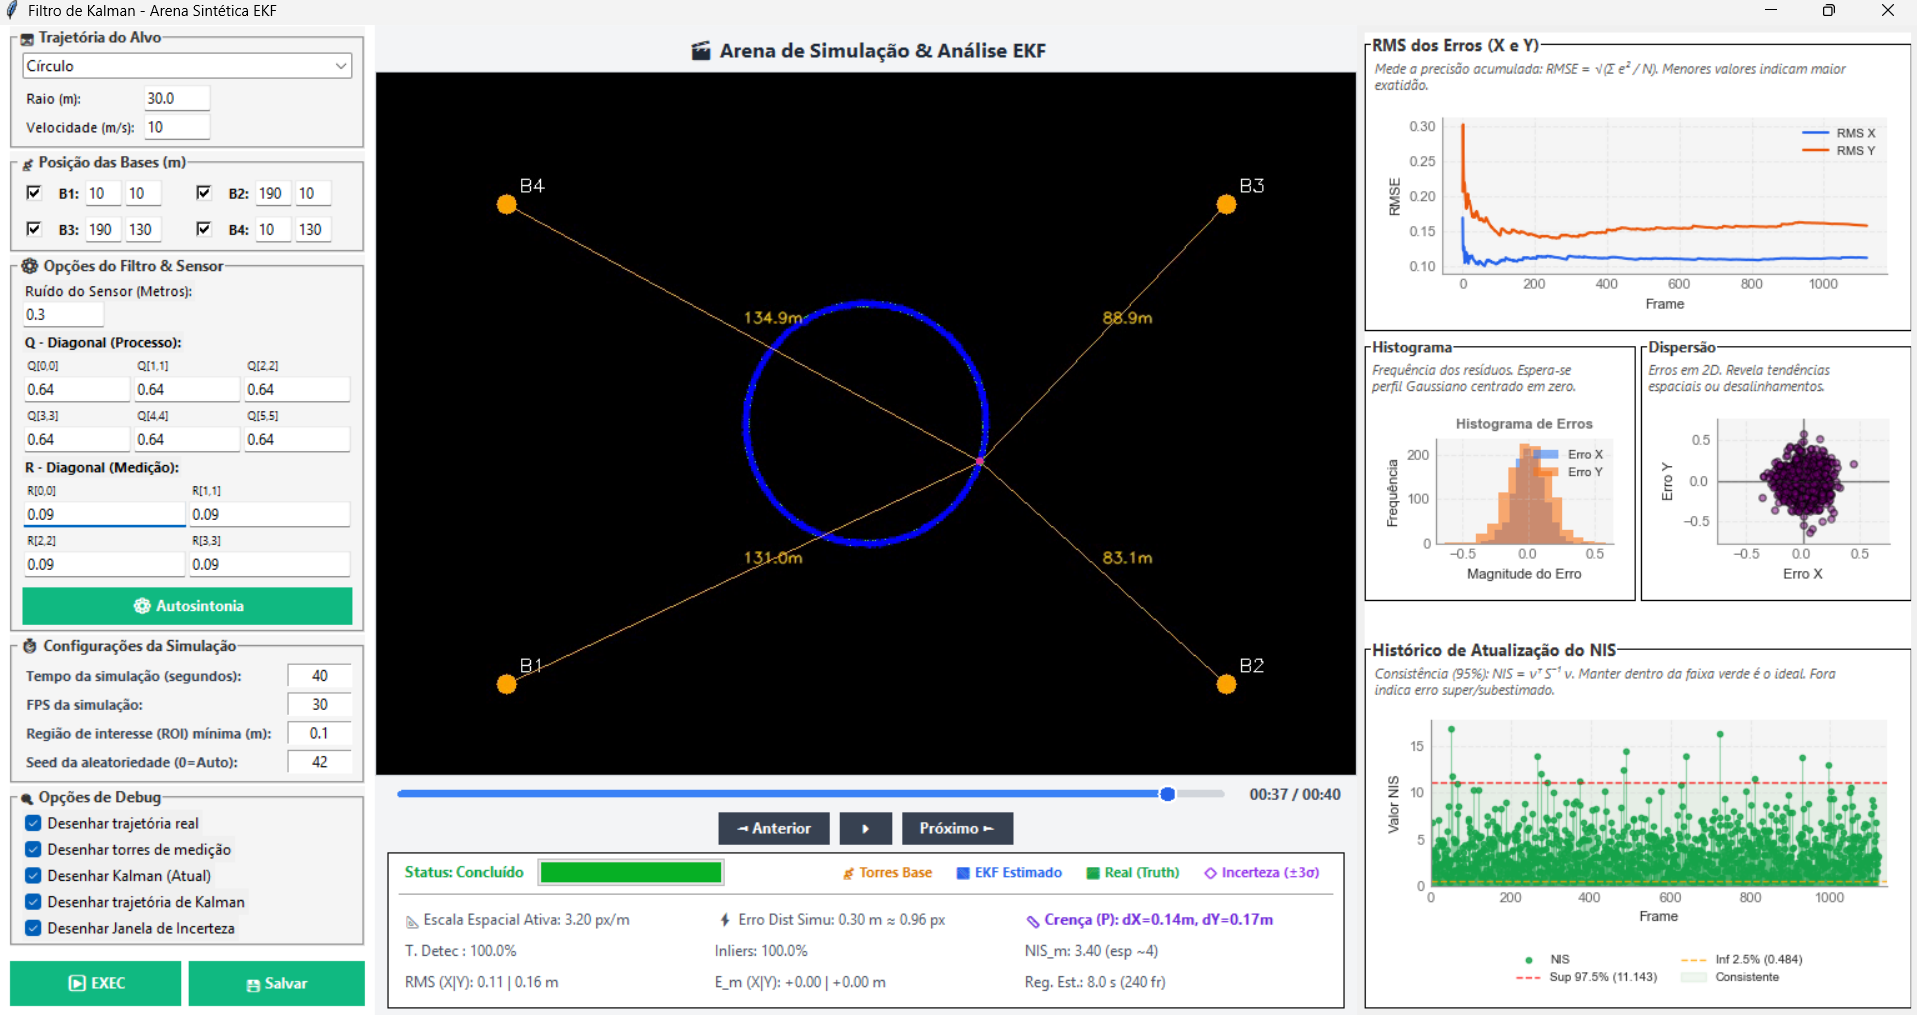
\includegraphics[width=0.9\linewidth]{Figuras/diagrams/Bases.png}
    \caption{Ambiente gráfico desenvolvido em Python. O painel central exibe a cinemática do alvo, ladeado pelos controles de simulação à esquerda e gráficos de monitoramento temporal à direita.}
    \label{fig:gui_funcional}
\end{figure*}
% -------------------------------------------------------------

\subsection{Análise de Acurácia Posicional e Distribuição de Erros}
\label{subsec:accuracy_analysis}

A parametrização do EKF apresentou correlação direta com a mitigação do ruído de observação. Conforme os dados consolidados na Tabela \ref{tab:resumo_metricas_dividida_nomes} e as trajetórias detalhadas no Apêndice \ref{app:graficos_completos}, a configuração sintonizada manteve o $\text{RMSE}_x$ e o $\text{RMSE}_y$ em níveis sub-métricos estritos, com erros em $X$ variando entre $0{,}11$\,m e $0{,}13$\,m, e em $Y$ entre $0{,}14$\,m e $0{,}18$\,m nos cenários de visibilidade total. No Cenário 2 (Trajetória Quadrada), caracterizado por descontinuidades severas de aceleração ortogonal nos vértices, a sintonia correta demonstrou robustez ao conter o Erro Máximo Absoluto em $0{,}58$\,m. Em contrapartida, a configuração não sintonizada sob regime lento ($Q=0{,}01; R=0{,}10$) falhou em acompanhar as transições abruptas, resultando em um salto do RMSE para $0{,}60$\,m em $X$ e $0{,}82$\,m em $Y$, além de registrar um pico de erro máximo de $2{,}24$\,m devido ao atraso de fase clássico.

A evolução temporal dessa métrica é detalhada na Figura \ref{fig:rmse_temporal}, onde a curva de erro da condição calibrada permanece estável e contida dentro da margem operacional prevista.

\begin{figure}[htpb]
    \centering
    
\includegraphics[width=0.9\linewidth]{Figuras/C2/sintonizado/simulacao_quadrado_2_rms.png}
    \caption{Evolução temporal do RMSE (Cenário 2). A estabilidade da curva reflete a consistência do filtro quando devidamente sintonizado frente a manobras evasivas.}
    \label{fig:rmse_temporal}
\end{figure}

Para aprofundar a avaliação do comportamento estatístico do estimador, a Figura \ref{fig:distribuicao_erros} apresenta o comportamento estocástico dos resíduos de predição. Nos gráficos de dispersão e histogramas associados à condição sintonizada, nota-se que os erros de estimação em X e Y se distribuem assintoticamente como uma normal bivariada, com viés médio estatisticamente nulo ($\mu_x \approx -0{,}00$\,m no cenário do quadrado). Quando a sintonia falha, a distribuição perde a sua característica gaussiana e exibe caudas pesadas ou dispersões deslocadas, refletindo o descompasso geométrico e o atraso de fase na estimação dos estados.

\begin{figure}[htpb]
    \centering
    
\includegraphics[width=0.9\linewidth]{Figuras/C2/sintonizado/simulacao_quadrado_5_hist.png}
    \vspace{1mm}
    \\{\small (a) Condição Sintonizada}
    \vspace{6mm}
    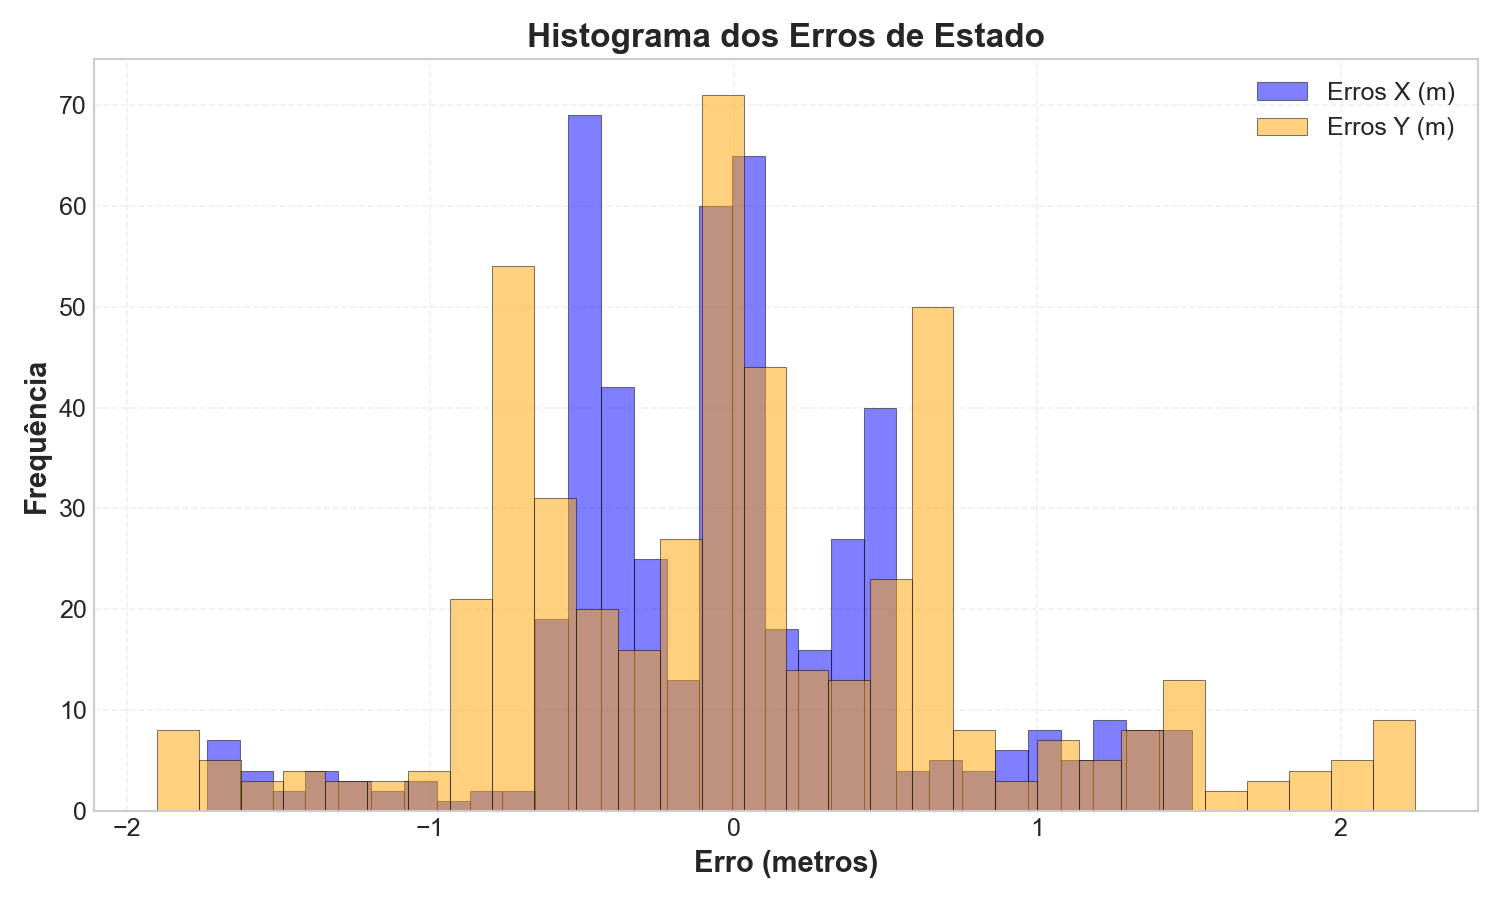
\includegraphics[width=0.9\linewidth]{Figuras/C2/nsintonizado/simulacao_quadrado_5_hist.png}
    \vspace{1mm}
    \\{\small (b) Condição Não Sintonizada}
    \caption{Histogramas e dispersão dos erros de predição (Cenário 2). Em (a), a condição sintonizada converge para uma distribuição normal centrada no zero. Em (b), a ausência de calibração induz dispersão irregular e acúmulo de erros de fase.}
    \label{fig:distribuicao_erros}
\end{figure}

\subsection{Consistência Estatística e Monitoramento do NIS}
\label{subsec:nis_analysis}

A coerência entre a incerteza teórica calculada pelo filtro e os resíduos de inovação reais foi avaliada por meio da estatística \textit{Normalized Innovation Squared} (NIS). Para o modelo rastreado por quatro torres ativas (4 graus de liberdade), a esperança teórica do NIS é exatamente $\mathbb{E}[NIS] = 4{,}0$. O limite crítico superior bicaudal para um nível de confiança de $95\%$ situa-se em $\chi^2_{0.975, 4} = 11{,}143$.

Como ilustra a Figura \ref{fig:nis_evolucao} e os dados da Tabela \ref{tab:resumo_metricas_dividida_nomes}, o EKF sintonizado demonstrou alto equilíbrio e consistência estatística. Os valores médios operacionais ($\overline{NIS}$) flutuaram estavelmente entre $3{,}34$ e $3{,}86$, aproximando-se com rigor do valor teórico esperado de $4{,}0$. As taxas de violação do limite superior permaneceram estritamente controladas (entre $0{,}75\%$ e $2{,}29\%$), validando estatisticamente a matriz de covariância do erro de estimação $\mathbf{P}$.

Por outro lado, o perfil não sintonizado expôs dois comportamentos patológicos distintos: nos cenários de subestimação drástica do ruído de leitura ($R=0{,}01$ nos Cenários 3 a 6), o filtro operou em regime severamente otimista. A média do NIS disparou (atingindo $31{,}67$ no Cenário 6), com taxas de violação do limite crítico que superaram $84\%$. Nos cenários com superestimação de $R$ combinada com redução de $Q$ (Cenários 1 e 2), o filtro tendeu à lentidão e perda de reatividade, acumulando inovações elevadas que inflaram o $\overline{NIS}$ para $24{,}07$ no Cenário 2, estourando o limite em mais de $50\%$ das amostras.

\begin{figure}[htpb]
    \centering
    
\includegraphics[width=0.9\linewidth]{Figuras/C3/sintonizado/simulacao_tangente_hiperbólica_4_nis.png}
    \caption{Comportamento temporal da métrica NIS. A calibração adequada mantém o parâmetro próximo à média teórica ($4,0$) e abaixo do limite crítico superior ($11,14$).}
    \label{fig:nis_evolucao}
\end{figure}

\subsection{Região de Confiança e Taxa de Inliers}
\label{subsec:inliers_analysis}

A Taxa de \textit{Inliers} (TI) quantificou a porcentagem de frames em que o erro real de posicionamento esteve contido dentro da elipse de confiança calculada pelo filtro. Nos cenários sintonizados, em decorrência da calibração exata das covariâncias, a TI apresentou desempenho ótimo, cravando $100{,}00\%$ nas trajetórias suaves (Cenários 1, 3, 4, 5 e 6) e mantendo-se em patamar seguro de $96{,}88\%$ na severa geometria do quadrado. Isso assegura que as elipses geradas pelo estimador refletem de forma fiel a dispersão espacial do erro. Na condição descalibrada dos Cenários 1 e 2, o estreitamento incorreto das elipses combinado ao atraso físico da trajetória fez a região de confiança colapsar, derrubando a TI para níveis críticos de $10{,}08\%$ e $28{,}07\%$, respectivamente.

\subsection{Resposta Transitória sob Oclusão (Cenário 6)}
\label{subsec:occlusion_analysis}

O Cenário 6 validou a estabilidade do algoritmo em malha aberta ao impor uma janela de oclusão temporária de sinal, reduzindo a Taxa de Detecção (TD) global para $90\%$. A Figura \ref{fig:analise_oclusao} detalha o intervalo de interrupção das medições. A modelagem cinemática consistente permitiu que a propagação de estados estimasse a posição puramente preditiva com base nas últimas velocidades calculadas. Embora o afastamento temporário do sinal tenha expandido o erro máximo absoluto para $2{,}62$\,m no ápice da oclusão, o sistema evitou o colapso numérico e restabeleceu a convergência sub-métrica imediatamente após a reconexão com as balizas, mantendo um RMSE global controlado de $0{,}17$\,m em $X$ e $0{,}34$\,m em $Y$.

\begin{figure}[htpb]
    \centering
    
\includegraphics[width=0.9\linewidth]{Figuras/C6/sintonizado/simulacao_oclusão_1_traj.png}
    \caption{Recorte do Cenário 6 sob oclusão temporária. O EKF propaga a cinemática em malha aberta sem divergência crítica.}
    \label{fig:analise_oclusao}
\end{figure}

% Capítulo 6: Conclusão
% ============================================================
% CAPÍTULO 6: CONCLUSÃO
% ============================================================

\section{Conclusão}
\label{sec:conclusion}

\subsection{Resumo e Principais Constatações}
\label{subsec:summary_findings}

Este trabalho analisou o comportamento de um Filtro de Kalman Estendido (EKF) sob o modelo Posição-Velocidade-Aceleração (PVA) no rastreamento 2D com medições \textit{range-only}. Em condições ideais de sintonia ($\mathbf{Q}=0{,}64$ e $\mathbf{R}=0{,}09$), o sistema apresentou alta precisão espacial (RMSE abaixo de $0{,}34$\,m) e consistência estatística (NIS dentro do intervalo de confiança em mais de $95\%$ do tempo), além de lidar com robustez em cenários de oclusão graças à inércia mecânica do modelo.

A principal descoberta, evidenciada ao descalibrar as matrizes intencionalmente, foi o claro desacoplamento entre precisão visual e coerência matemática. Subestimar a covariância de processo ($\mathbf{Q}=0{,}01$) engessa o filtro, fazendo a Taxa de \textit{Inliers} desabar para cerca de $10\%$ por gerar elipses de incerteza artificialmente pequenas. Já a subestimação da medição ($\mathbf{R}=0{,}01$) cria uma falsa sensação de acerto: o filtro persegue o ruído às cegas, mantendo o RMSE baixo e os \textit{Inliers} acima de $93\%$. No entanto, ele opera em completa inconsistência matemática, uma falha crítica que só é exposta pelo fato do NIS estourar o limite de $11{,}143$.

\subsection{Contribuições}
\label{subsec:contributions}

As principais entregas desta pesquisa incluem:
\begin{itemize}
    \item O desenvolvimento de um ambiente de simulação capaz de renderizar elipses de incerteza e auditar matrizes de covariância em tempo real.
    \item A consolidação do uso conjunto de RMSE e NIS como ferramenta definitiva de diagnóstico, provando que erros de posição aparentes não bastam para validar o filtro.
    \item A formulação da Taxa de \textit{Inliers} a partir de uma Região de Interesse (ROI) Dinâmica. Além de mensurar a coerência da crença do robô, essa estratégia abre um caminho promissor para sistemas de visão computacional, permitindo que o algoritmo processe apenas recortes preditivos da imagem.
\end{itemize}

\subsection{Limitações e Trabalhos Futuros}
\label{subsec:limitations_future}

O estudo limitou-se a modelar os ruídos como puramente gaussianos, desconsiderando distúrbios severos encontrados na prática (como efeitos de \textit{multipath} e NLOS em redes UWB), além de ter adotado um processo de calibração manual empírico. 

Para solucionar essas lacunas e expandir o projeto, sugerem-se as seguintes frentes de trabalho:
\begin{itemize}
    \item \textbf{Sintonia Automática:} Implementar algoritmos de otimização matemática (como descida de gradiente ou algoritmos genéticos) para sintonizar $\mathbf{Q}$ e $\mathbf{R}$ de forma totalmente autônoma.
    \item \textbf{Integração com Visão Computacional Prática:} Empregar a ROI preditiva calculada pelo EKF em fluxos reais de processamento de câmera para quantificar ganhos práticos em \textit{Frames Por Segundo} (FPS).
    \item \textbf{Filtros Avançados:} Comparar este EKF com estimadores que não dependem do cálculo de matrizes Jacobianas para contornar dinâmicas altamente não lineares, como o Filtro de Kalman \textit{Unscented} (UKF) ou Filtros de Partículas.
\end{itemize}

\subsection{Conclusão Final}
\label{subsec:final_conclusion}

Em suma, projetar um bom estimador significa entender que quantificar a própria incerteza de maneira realista é tão vital quanto calcular a coordenada final do alvo. O equilíbrio entre a precisão macroespacial do RMSE e a auditoria interna do NIS, aliado às otimizações viabilizadas pela Taxa de \textit{Inliers}, consolida uma base metodológica segura e eficiente para o avanço de algoritmos em robótica móvel e sistemas embarcados.

% ============================================================
% REFERÊNCIAS BIBLIOGRÁFICAS
% ============================================================

\bibliographystyle{IEEEtran}
\bibliography{referencias}


% ============================================================
% APÊNDICES
% ============================================================
\appendices

\section{Material Suplementar e Repositório do Código}
\label{apendice:material_suplementar}

O código-fonte completo da ferramenta de simulação desenvolvida neste trabalho está disponível publicamente para consulta e reprodução dos testes. O repositório inclui a interface gráfica (GUI) em Python, os scripts de geração das trajetórias e a implementação matemática do EKF. 

Também foram disponibilizados no link os gráficos de todas as simulações em alta resolução, incluindo as trajetórias espaciais e as métricas do NIS que não couberam na íntegra ao longo do texto.

O acesso ao código e aos dados adicionais pode ser feito pelo link:

\begin{center}
    \url{https://github.com/SauloJose/PASKalmanTra}
\end{center}

No repositório \cite{silva2026ferramenta}, é possível rodar o simulador localmente para interagir com o ajuste das matrizes $\mathbf{Q}$ e $\mathbf{R}$, além de acompanhar a variação dinâmica da janela de ROI e das elipses de incerteza do filtro em tempo real.

% Se você possui os gráficos detalhados do capítulo de Resultados neste arquivo:
\section{Mapeamento Visual e Estatístico Completo}
\label{app:graficos_completos}

Este apêndice reúne os gráficos das trajetórias espaciais e a evolução temporal do NIS para os seis cenários testados. 
A sequência de imagens permite comparar diretamente a precisão e a consistência do EKF sintonizado com o filtro descalibrado.
Com isso, fica evidente o impacto visual da parametrização incorreta sobre as elipses de incerteza e os erros do sistema.

% ==============================================================
% PÁGINA 1: TODAS AS TRAJETÓRIAS (SINTONIZADAS E NÃO SINTONIZADAS) - SEM ALTERAÇÃO DE TAMANHO
% ==============================================================
\begin{figure*}[!htpb]
    \centering
    
    % --- PARTE A: SINTONIZADAS ---
    % Linha 1
    \begin{minipage}[b]{0.24\linewidth}
        \centering
        
\includegraphics[width=\linewidth]{Figuras/C1/sintonizado/simulacao_círculo_1_traj.png}
        \vspace{1mm} \par {\small (a) Círculo}
    \end{minipage}
    \hfill
    \begin{minipage}[b]{0.24\linewidth}
        \centering
        
\includegraphics[width=\linewidth]{Figuras/C2/sintonizado/simulacao_quadrado_1_traj.png}
        \vspace{1mm} \par {\small (b) Quadrado}
    \end{minipage}
    \hfill
    \begin{minipage}[b]{0.24\linewidth}
        \centering
        
\includegraphics[width=\linewidth]{Figuras/C3/sintonizado/simulacao_tangente_hiperbólica_1_traj.png}
        \vspace{1mm} \par {\small (c) Tangente Hiperbólica}
    \end{minipage}
    
    \vspace{3mm} % Espaço entre as linhas
    
    % Linha 2
    \begin{minipage}[b]{0.24\linewidth}
        \centering
        
\includegraphics[width=\linewidth]{Figuras/C4/sintonizado/simulacao_lemniscata_1_traj.png}
        \vspace{1mm} \par {\small (d) Lemniscata}
    \end{minipage}
    \hfill
    \begin{minipage}[b]{0.24\linewidth}
        \centering
        
\includegraphics[width=\linewidth]{Figuras/C5/sintonizado/simulacao_aleatória_1_traj.png}
        \vspace{1mm} \par {\small (e) Aleatória}
    \end{minipage}
    \hfill
    \begin{minipage}[b]{0.24\linewidth}
        \centering
        
\includegraphics[width=\linewidth]{Figuras/C6/sintonizado/simulacao_oclusão_1_traj.png}
        \vspace{1mm} \par {\small (f) Oclusão}
    \end{minipage}
    
    \caption{Trajetórias estimadas na \textbf{condição sintonizada}. Observa-se o rastreamento preciso da dinâmica do alvo e a mitigação contínua do ruído de observação, evidenciando o desempenho ideal do filtro.}
    \label{fig:app_traj_sintonizadas_grid}

    \vspace{8mm} % ESPAÇO ENTRE OS DOIS BLOCOS DE TRAJETÓRIA

    % --- PARTE B: NÃO SINTONIZADAS ---
    % Linha 1
    \begin{minipage}[b]{0.24\linewidth}
        \centering
        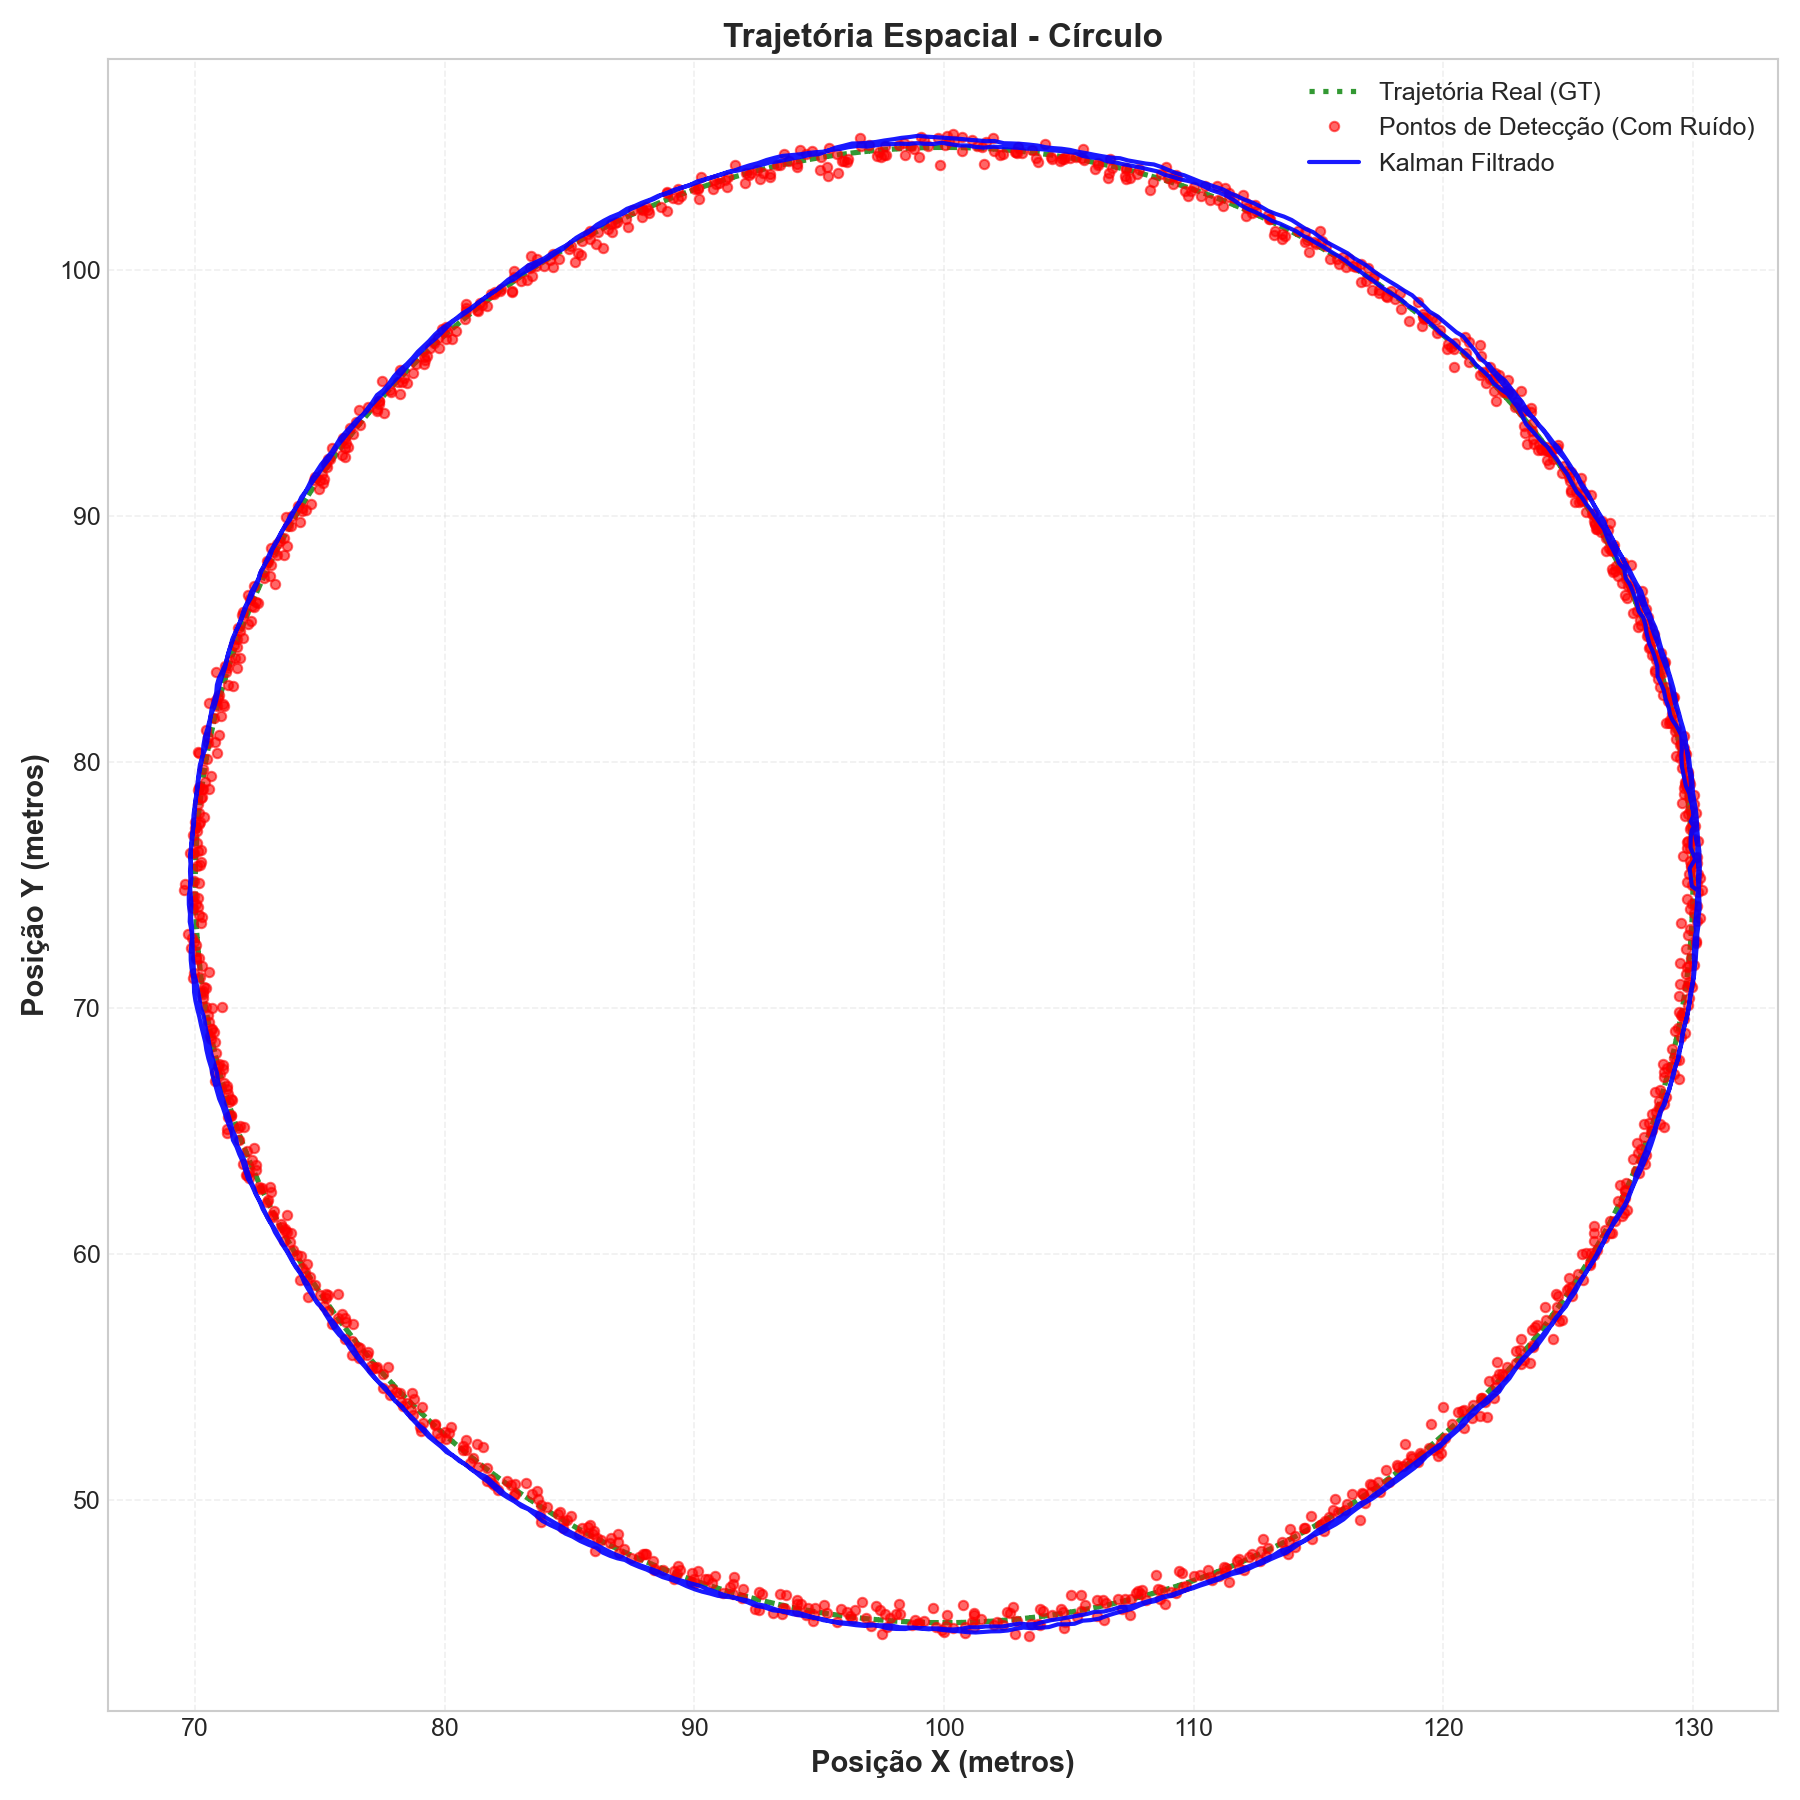
\includegraphics[width=\linewidth]{Figuras/C1/nsintonizado/simulacao_círculo_1_traj.png}
        \vspace{1mm} \par {\small (a) Círculo}
    \end{minipage}
    \hfill
    \begin{minipage}[b]{0.24\linewidth}
        \centering
        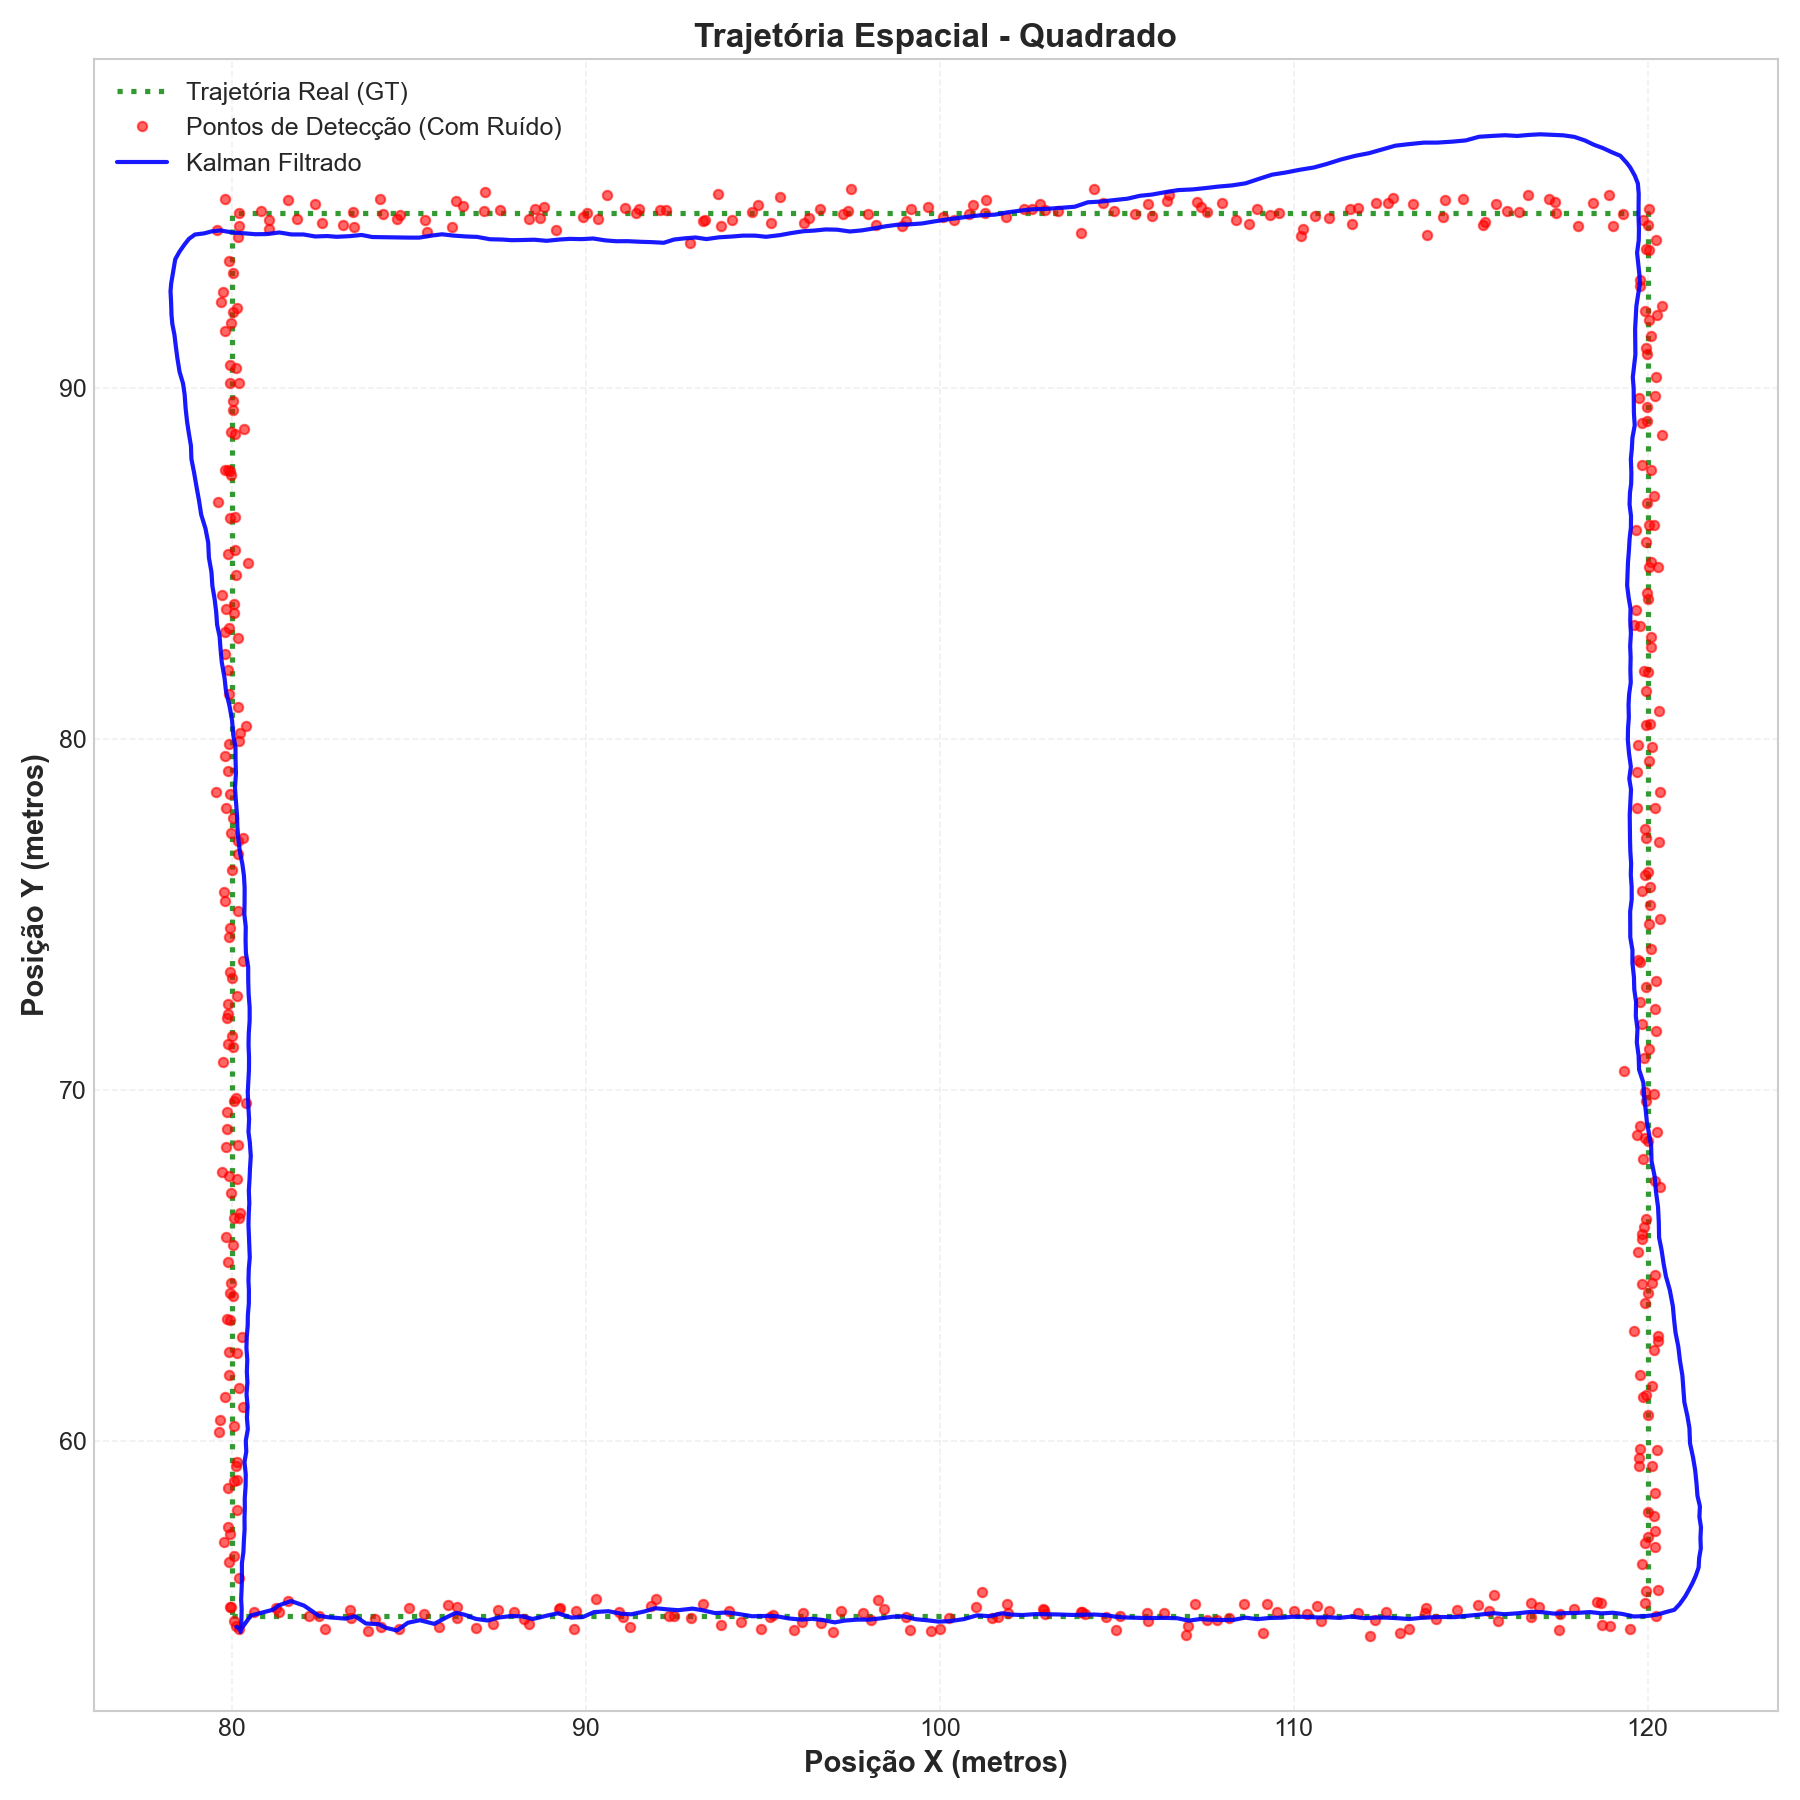
\includegraphics[width=\linewidth]{Figuras/C2/nsintonizado/simulacao_quadrado_1_traj.png}
        \vspace{1mm} \par {\small (b) Quadrado}
    \end{minipage}
    \hfill
    \begin{minipage}[b]{0.24\linewidth}
        \centering
        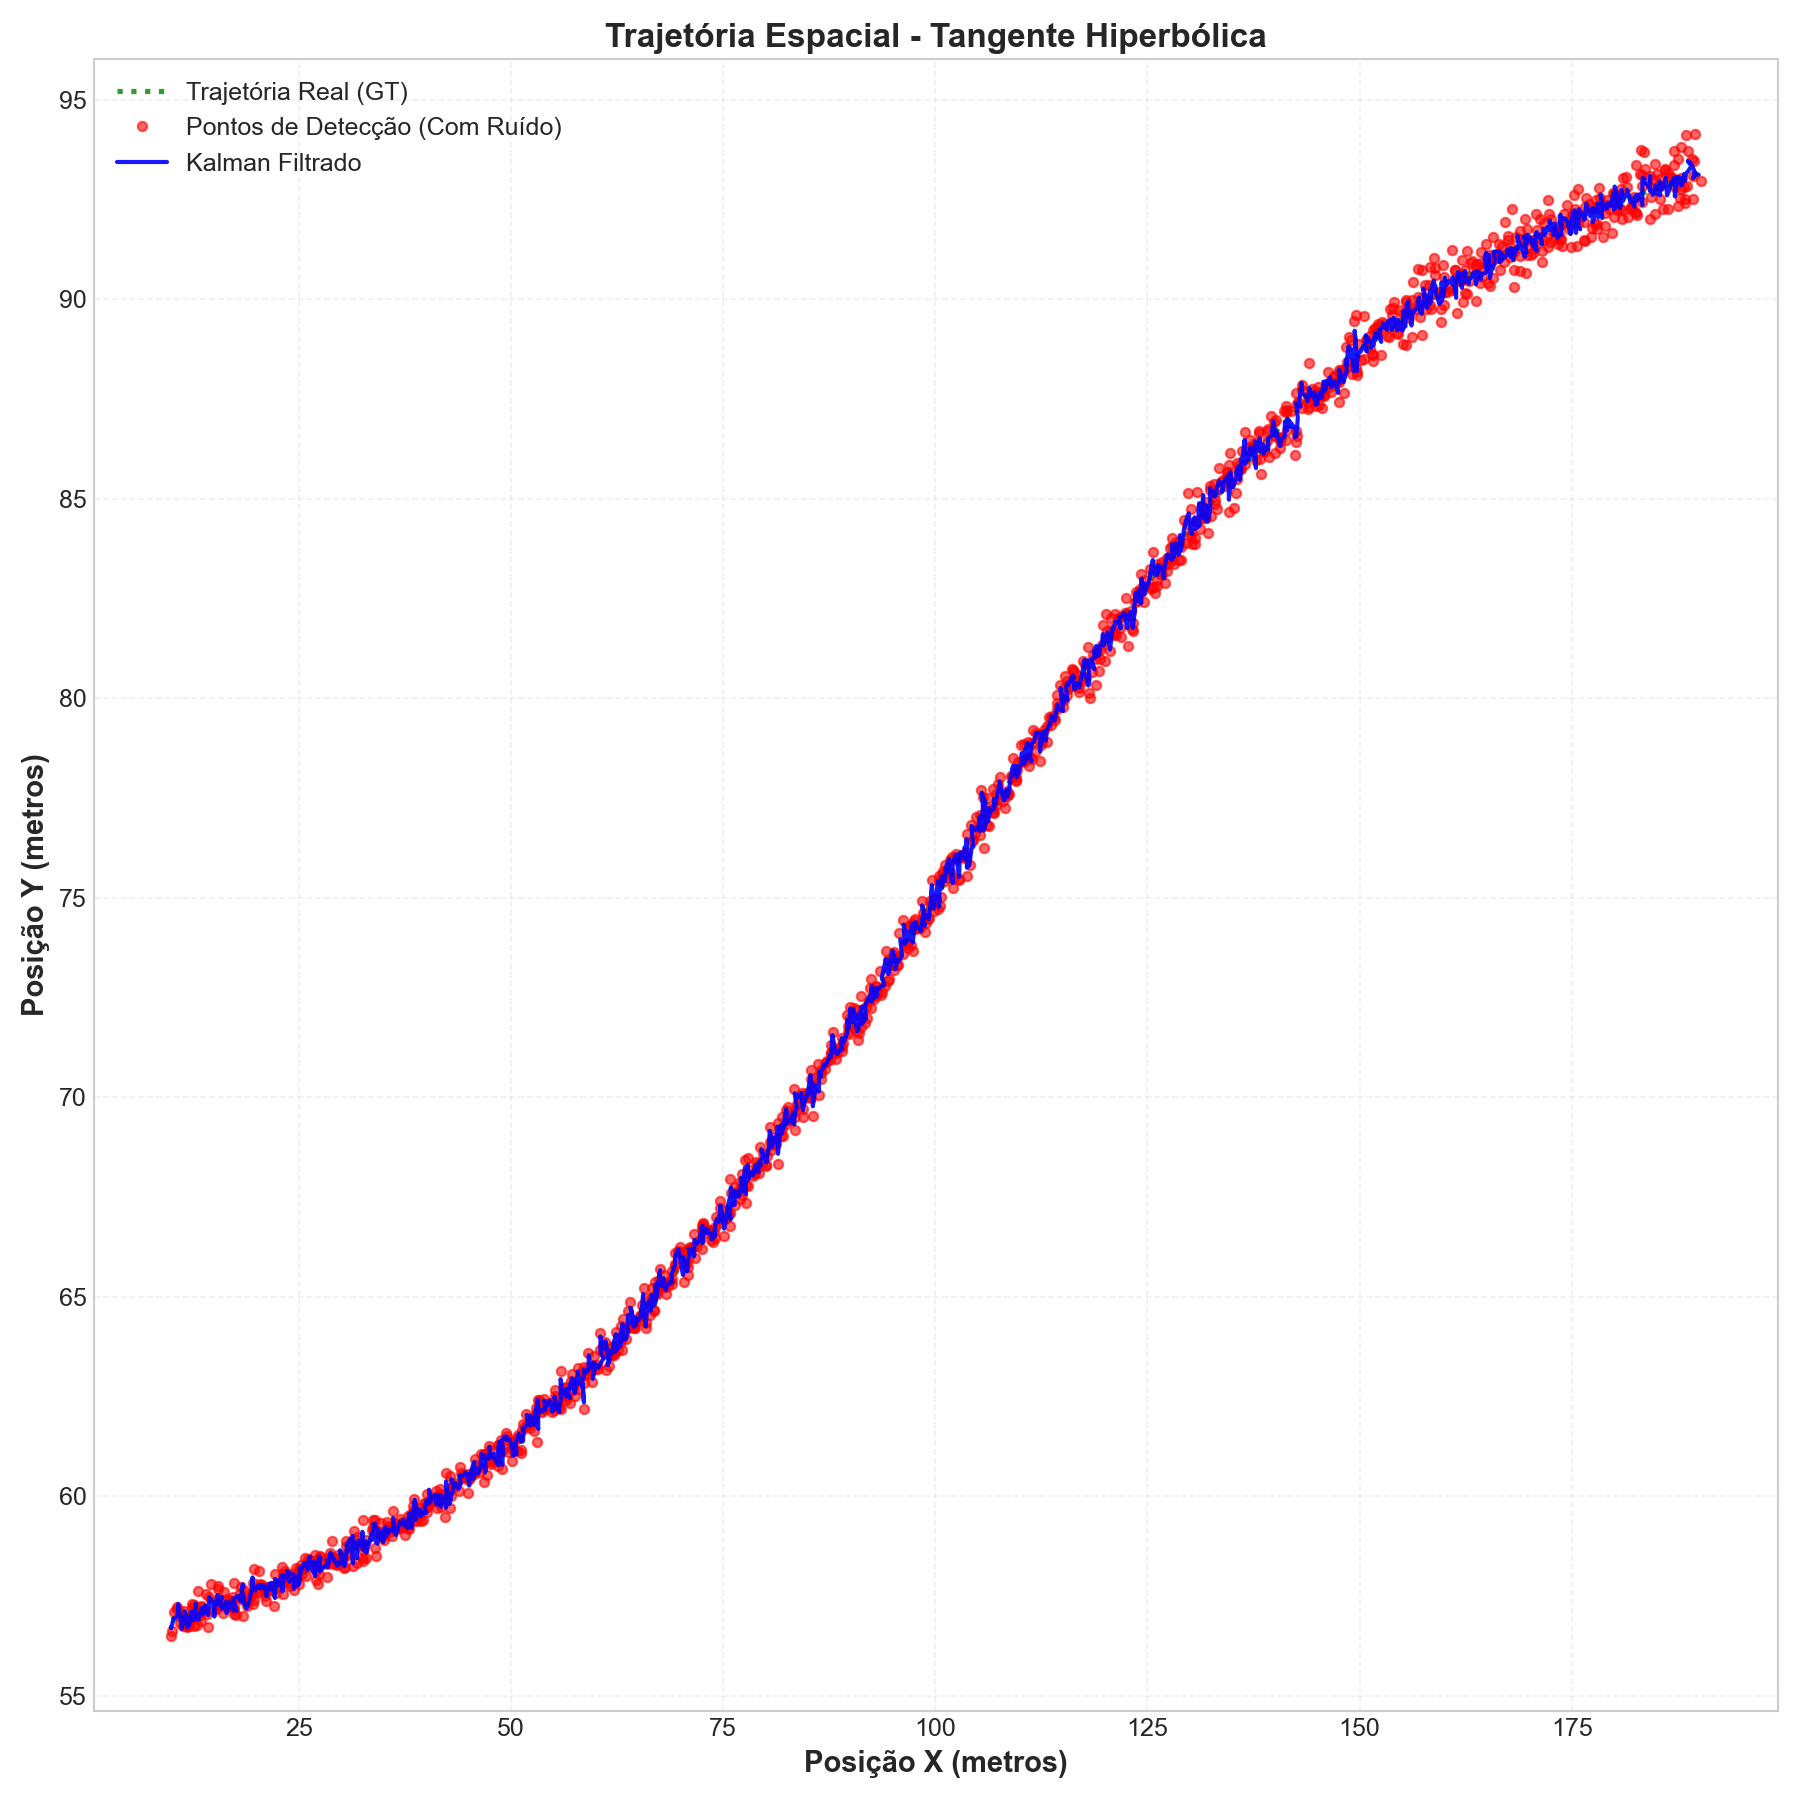
\includegraphics[width=\linewidth]{Figuras/C3/nsintonizado/simulacao_tangente_hiperbólica_1_traj.png}
        \vspace{1mm} \par {\small (c) Tangente Hiperbólica}
    \end{minipage}
    
    \vspace{3mm}
    
    % Linha 2
    \begin{minipage}[b]{0.24\linewidth}
        \centering
        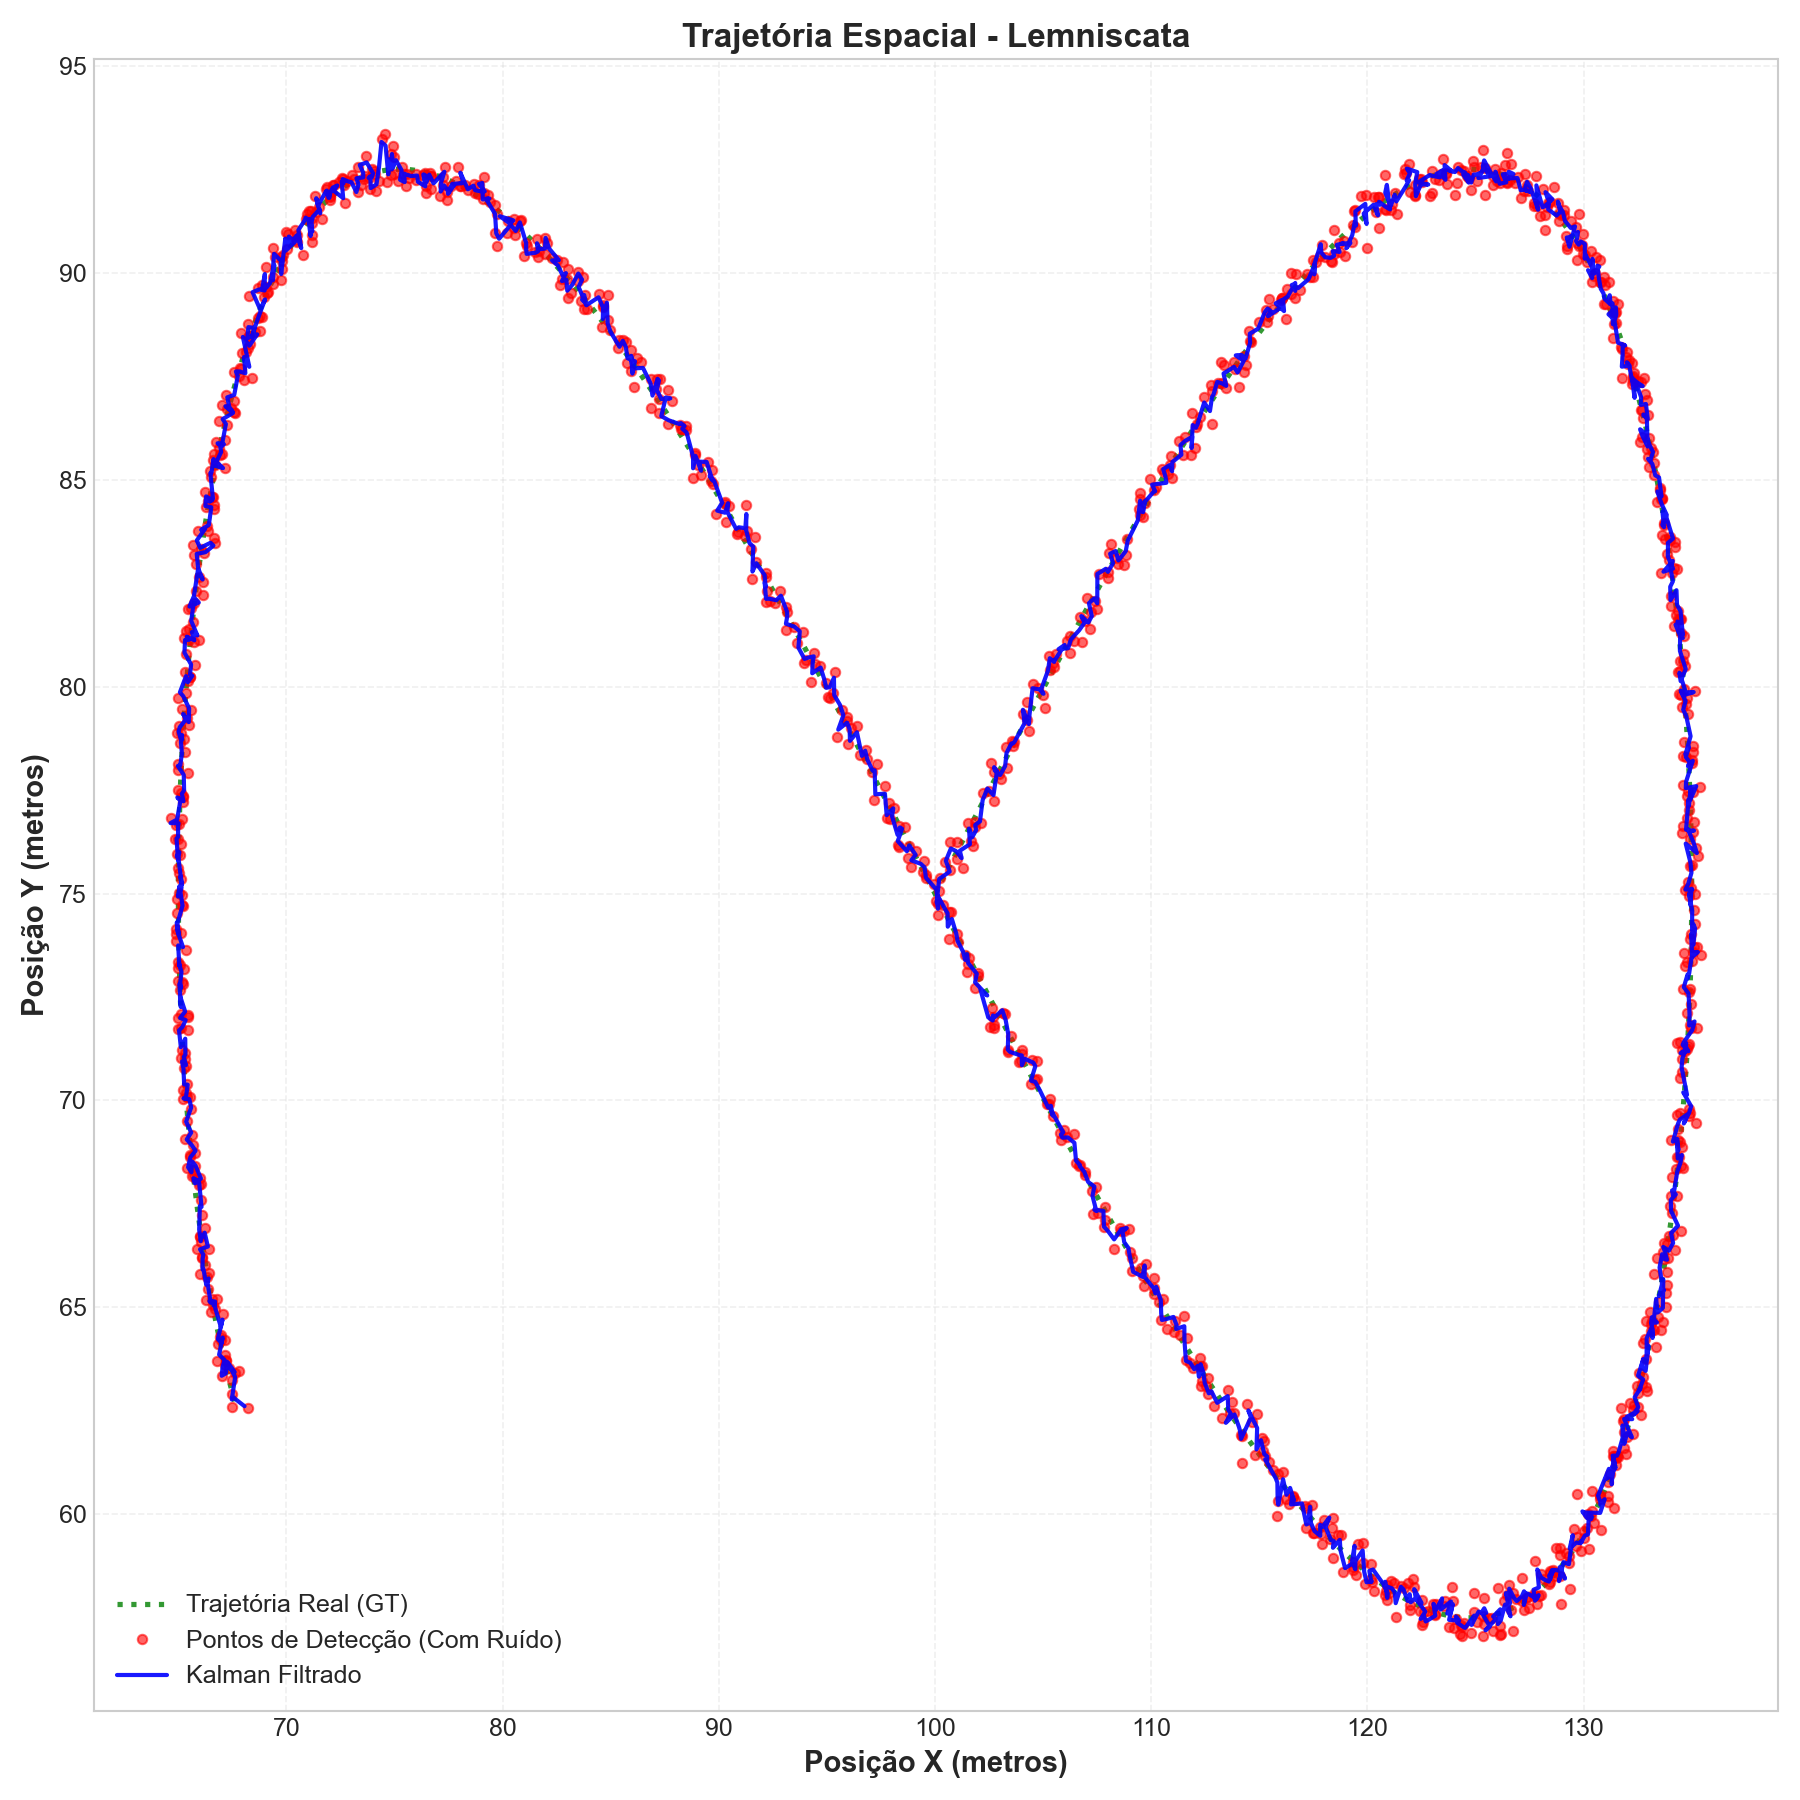
\includegraphics[width=\linewidth]{Figuras/C4/nsintonizado/simulacao_lemniscata_1_traj.png}
        \vspace{1mm} \par {\small (d) Lemniscata}
    \end{minipage}
    \hfill
    \begin{minipage}[b]{0.24\linewidth}
        \centering
        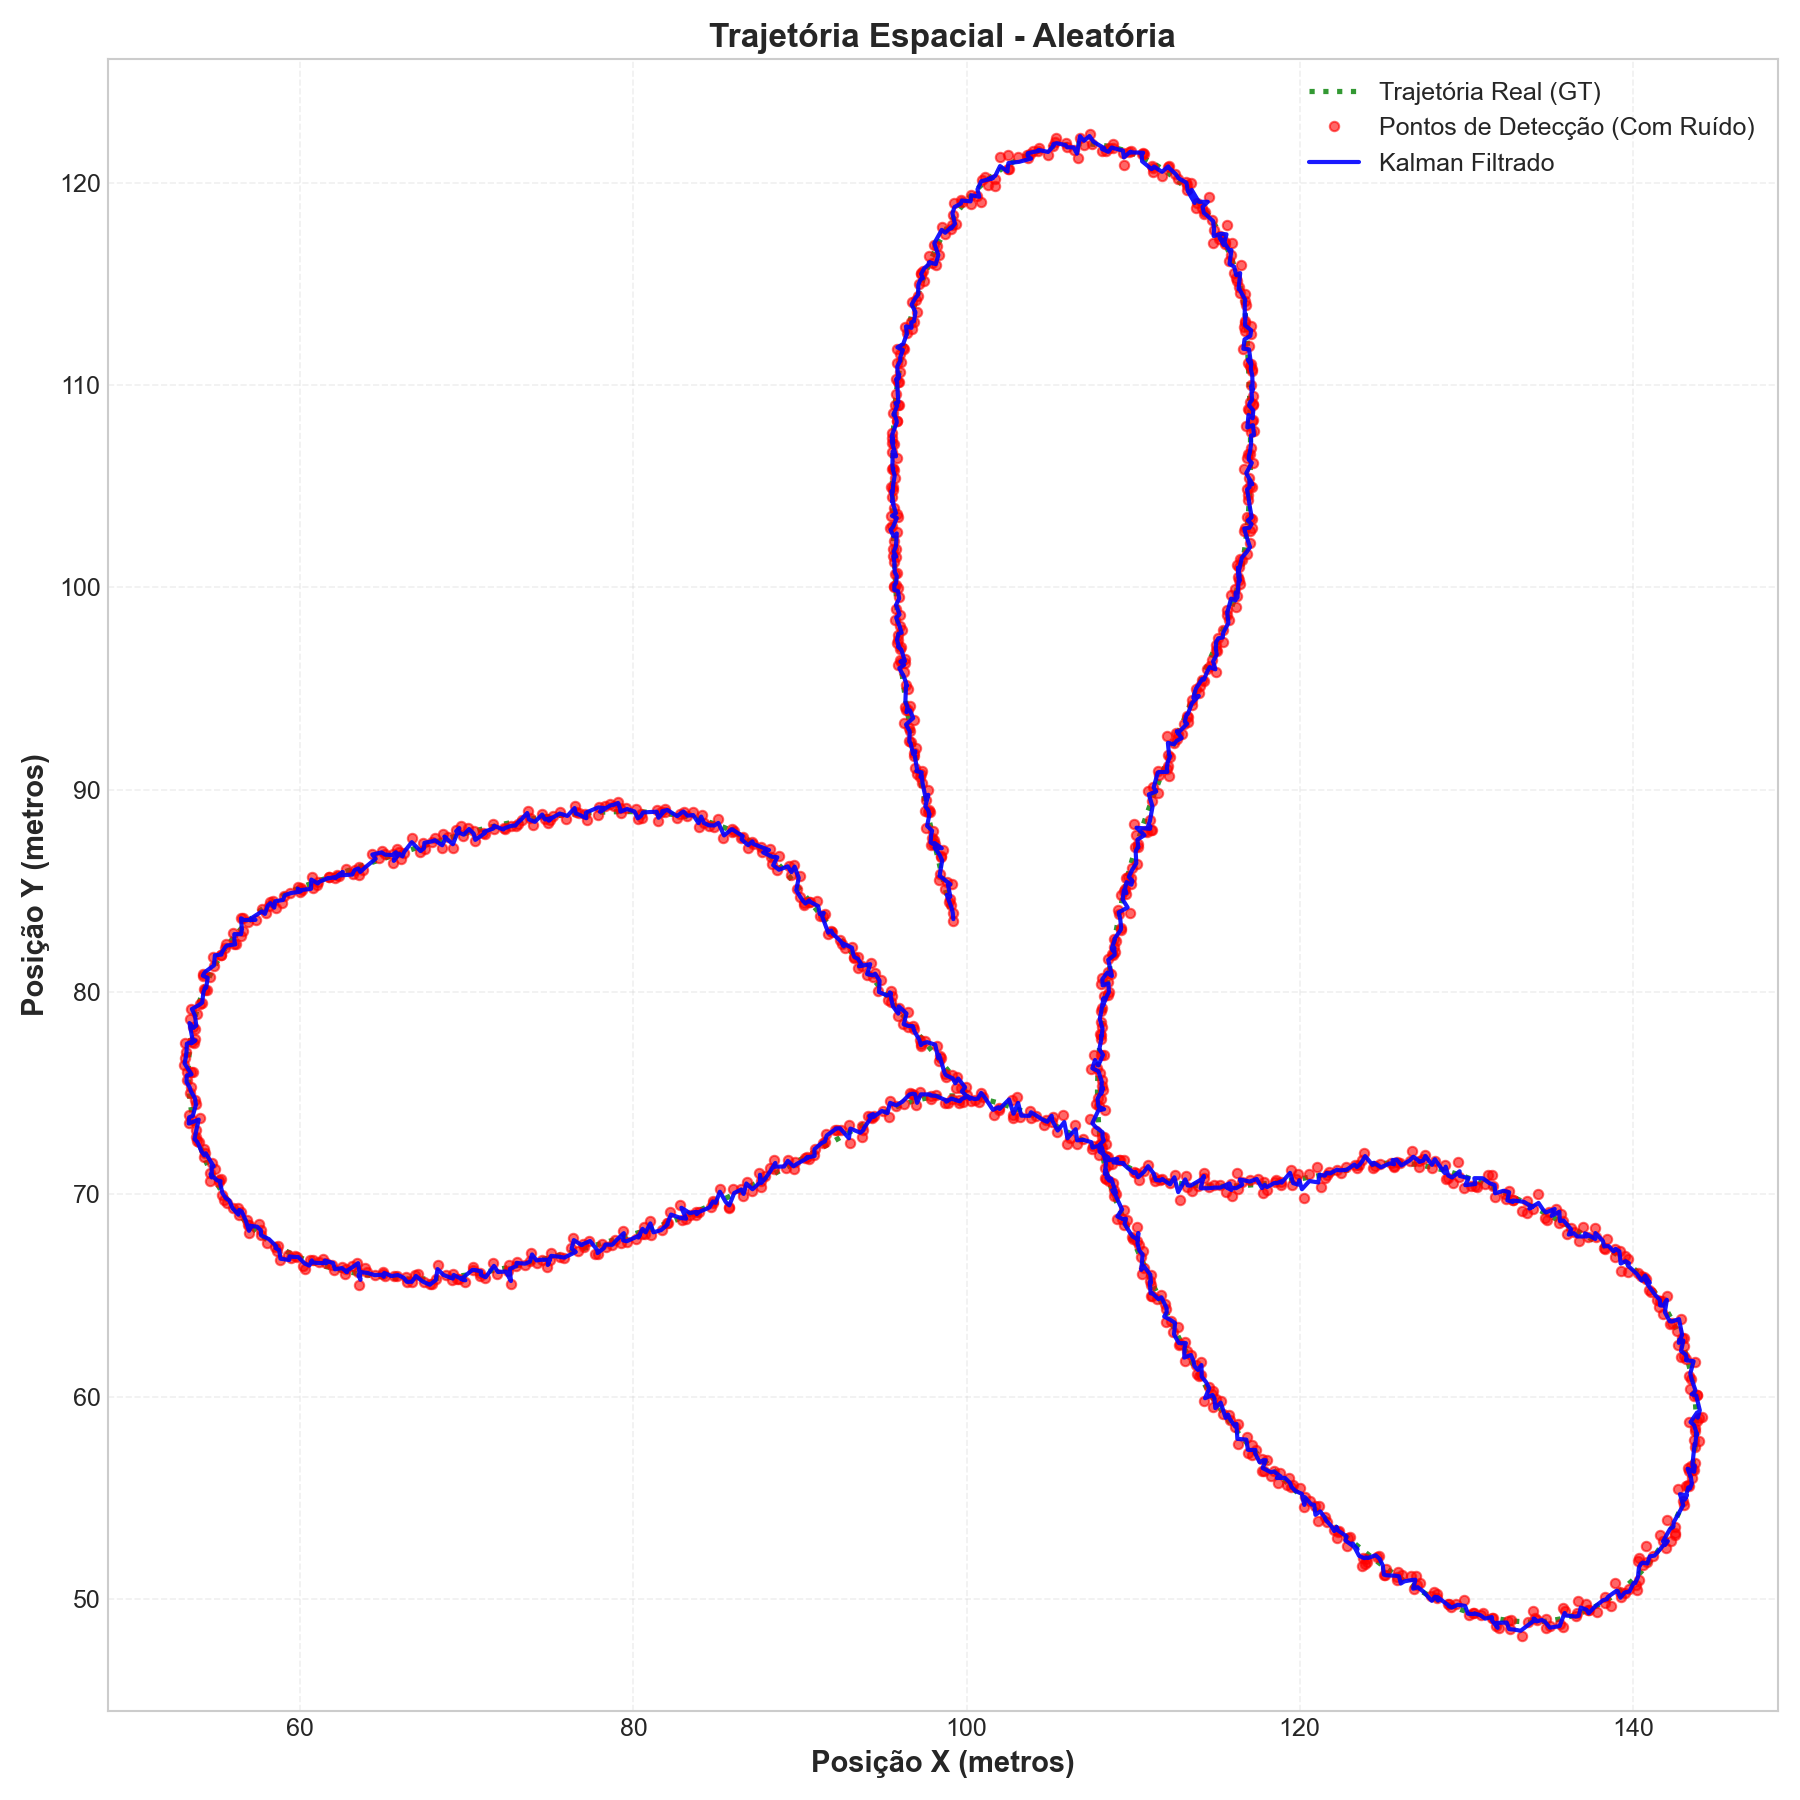
\includegraphics[width=\linewidth]{Figuras/C5/nsintonizado/simulacao_aleatória_1_traj.png}
        \vspace{1mm} \par {\small (e) Aleatória}
    \end{minipage}
    \hfill
    \begin{minipage}[b]{0.24\linewidth}
        \centering
        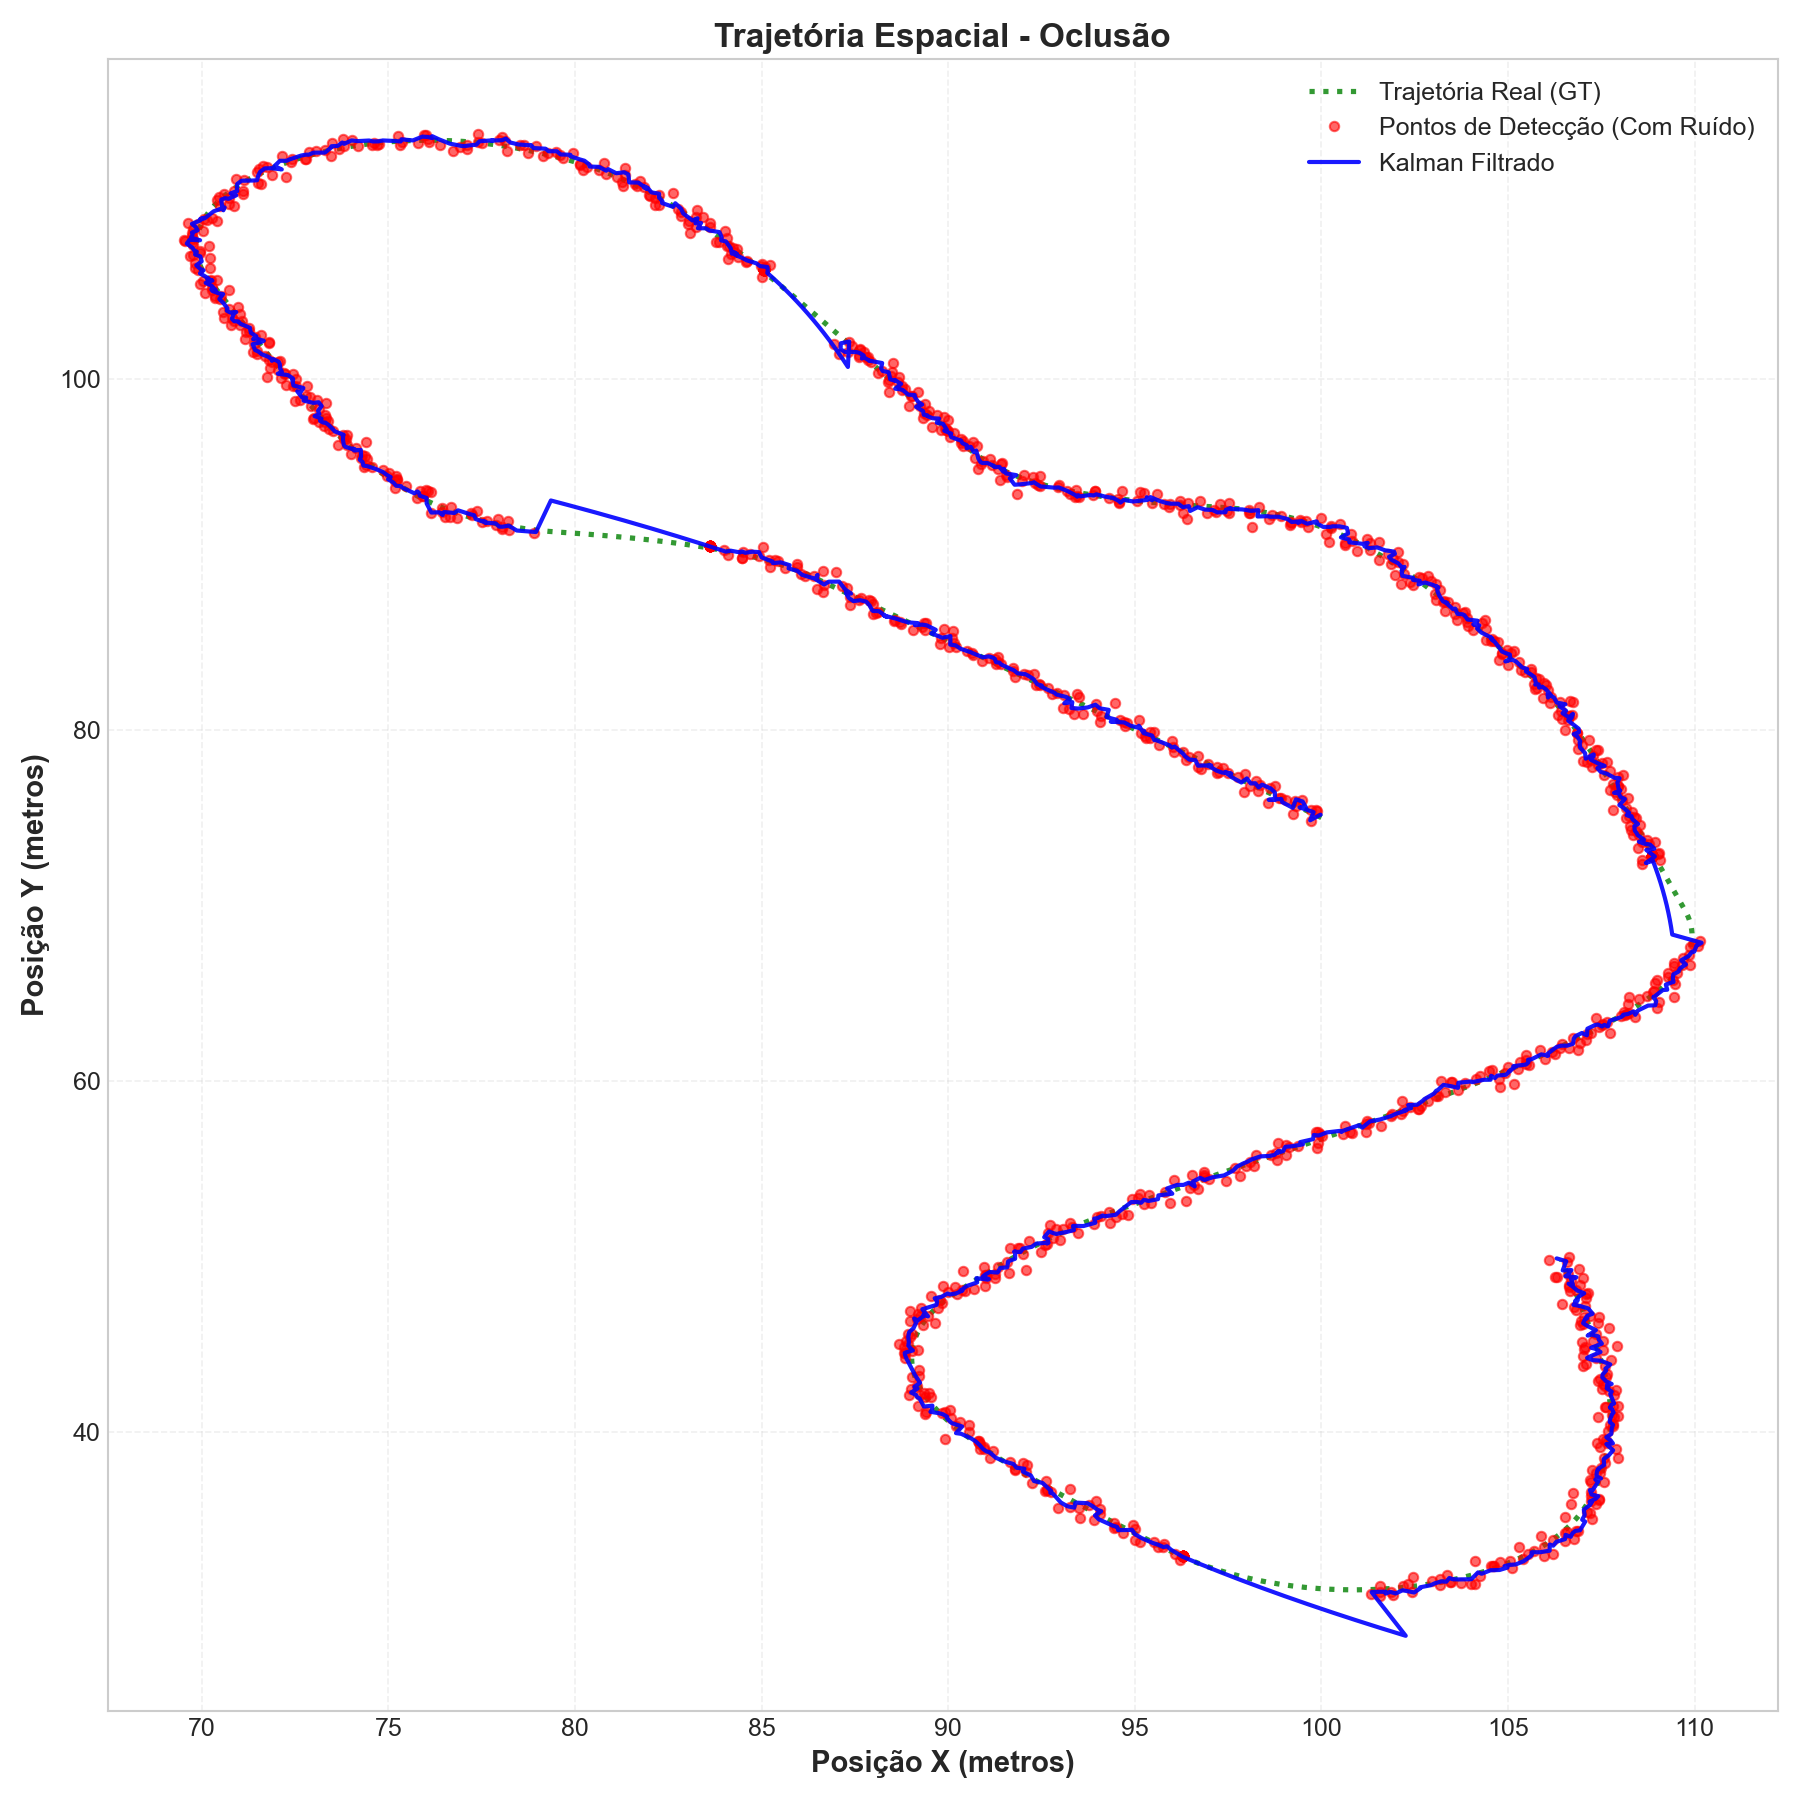
\includegraphics[width=\linewidth]{Figuras/C6/nsintonizado/simulacao_oclusão_1_traj.png}
        \vspace{1mm} \par {\small (f) Oclusão}
    \end{minipage}
    
    \caption{Trajetórias estimadas na \textbf{condição não sintonizada}. Notam-se divergências significativas em relação à verdade terrestre (\textit{ground truth}), com evidentes atrasos de fase e sobreposições bruscas nas curvas.}
    \label{fig:app_traj_naosintonizadas_grid}
\end{figure*}

% QUEBRA DE PÁGINA OBRIGATÓRIA
\clearpage


% ==============================================================
% PÁGINA 2: TODOS OS GRÁFICOS RMSE (SINTONIZADOS E NÃO SINTONIZADOS) - MAIORES
% ==============================================================
\begin{figure*}[!htpb]
    \centering
    
    % --- PARTE A: NIS SINTONIZADO ---
    % Linha 1
    \begin{minipage}[b]{0.32\linewidth}
        \centering
        
\includegraphics[width=\linewidth]{Figuras/C1/sintonizado/simulacao_círculo_2_rms.png}
        \vspace{1mm} \par {\small (a) Círculo}
    \end{minipage}
    \hfill
    \begin{minipage}[b]{0.32\linewidth}
        \centering
        
\includegraphics[width=\linewidth]{Figuras/C2/sintonizado/simulacao_quadrado_2_rms.png}
        \vspace{1mm} \par {\small (b) Quadrado}
    \end{minipage}
    \hfill
    \begin{minipage}[b]{0.32\linewidth}
        \centering
        
\includegraphics[width=\linewidth]{Figuras/C3/sintonizado/simulacao_tangente_hiperbólica_2_rms.png}
        \vspace{1mm} \par {\small (c) Tangente Hiperbólica}
    \end{minipage}
    
    \vspace{3mm}
    
    % Linha 2
    \begin{minipage}[b]{0.32\linewidth}
        \centering
        
\includegraphics[width=\linewidth]{Figuras/C4/sintonizado/simulacao_lemniscata_2_rms.png}
        \vspace{1mm} \par {\small (d) Lemniscata}
    \end{minipage}
    \hfill
    \begin{minipage}[b]{0.32\linewidth}
        \centering
        
\includegraphics[width=\linewidth]{Figuras/C5/sintonizado/simulacao_aleatória_2_rms.png}
        \vspace{1mm} \par {\small (e) Aleatória}
    \end{minipage}
    \hfill
    \begin{minipage}[b]{0.32\linewidth}
        \centering
        
\includegraphics[width=\linewidth]{Figuras/C6/sintonizado/simulacao_oclusão_2_rms.png}
        \vspace{1mm} \par {\small (f) Oclusão}
    \end{minipage}
    
    \caption{Evolução temporal da métrica RMSE para a \textbf{condição sintonizada}}
    \label{fig:app_rmse_sintonizado_grid}

    \vspace{8mm} % ESPAÇO ENTRE OS DOIS BLOCOS DE NIS

    % --- PARTE B: NIS NÃO SINTONIZADO ---
    % Linha 1
    \begin{minipage}[b]{0.32\linewidth}
        \centering
        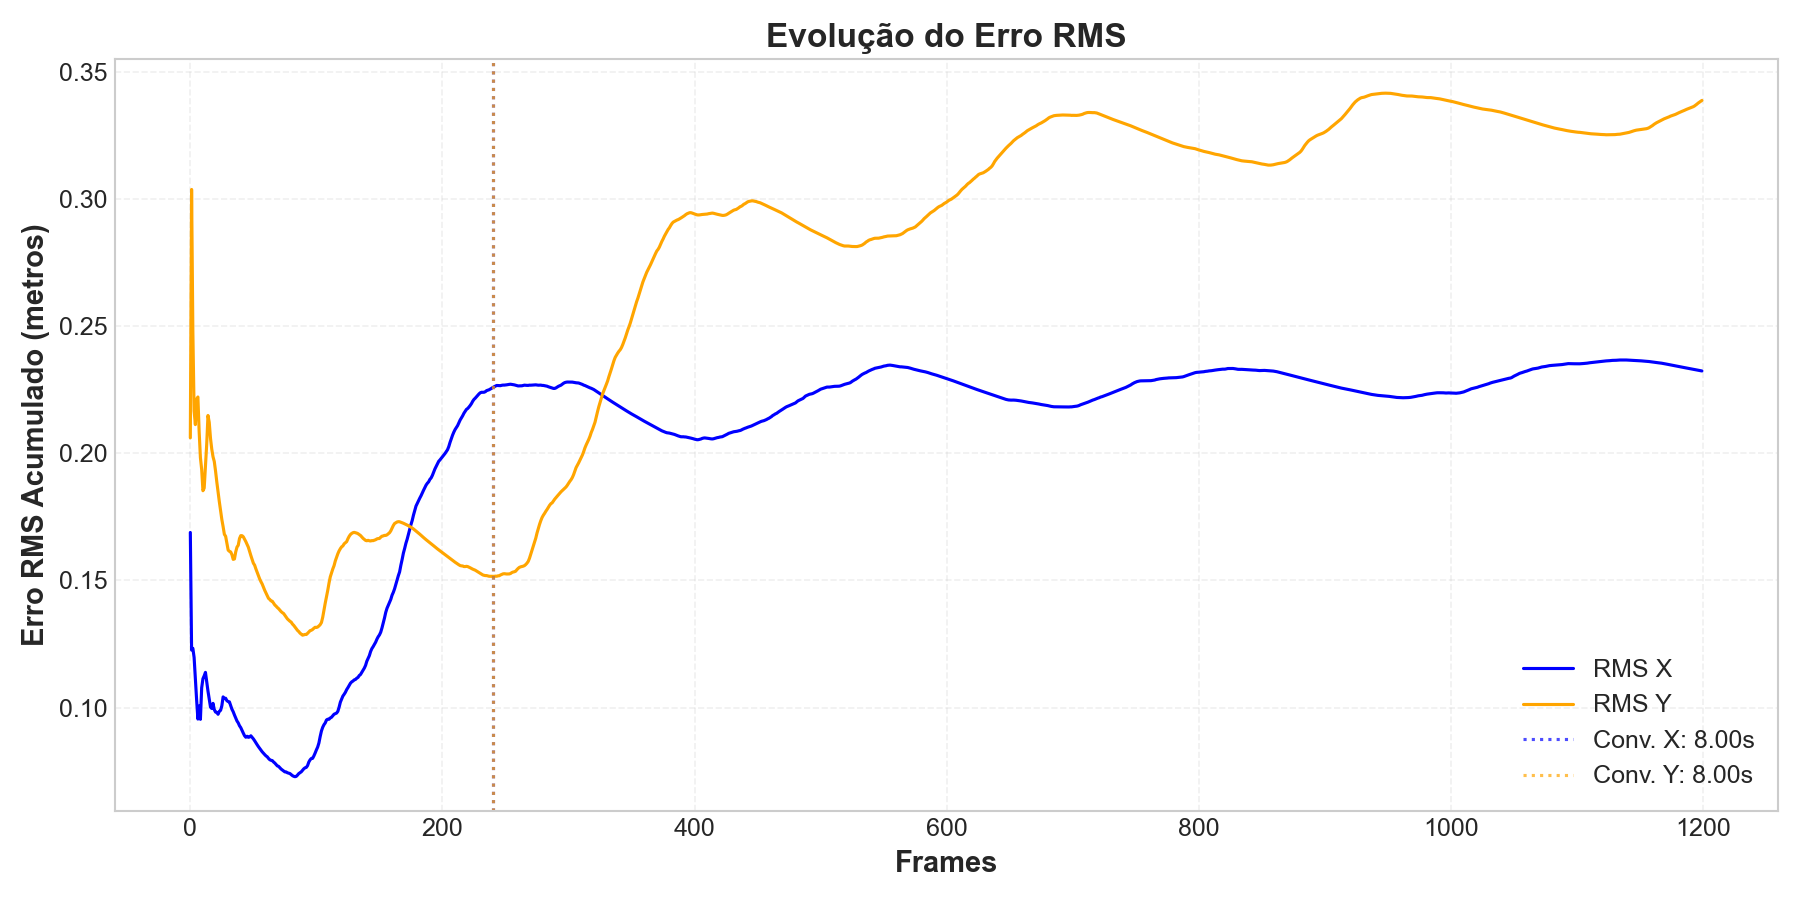
\includegraphics[width=\linewidth]{Figuras/C1/nsintonizado/simulacao_círculo_2_rms.png}
        \vspace{1mm} \par {\small (a) Círculo}
    \end{minipage}
    \hfill
    \begin{minipage}[b]{0.32\linewidth}
        \centering
        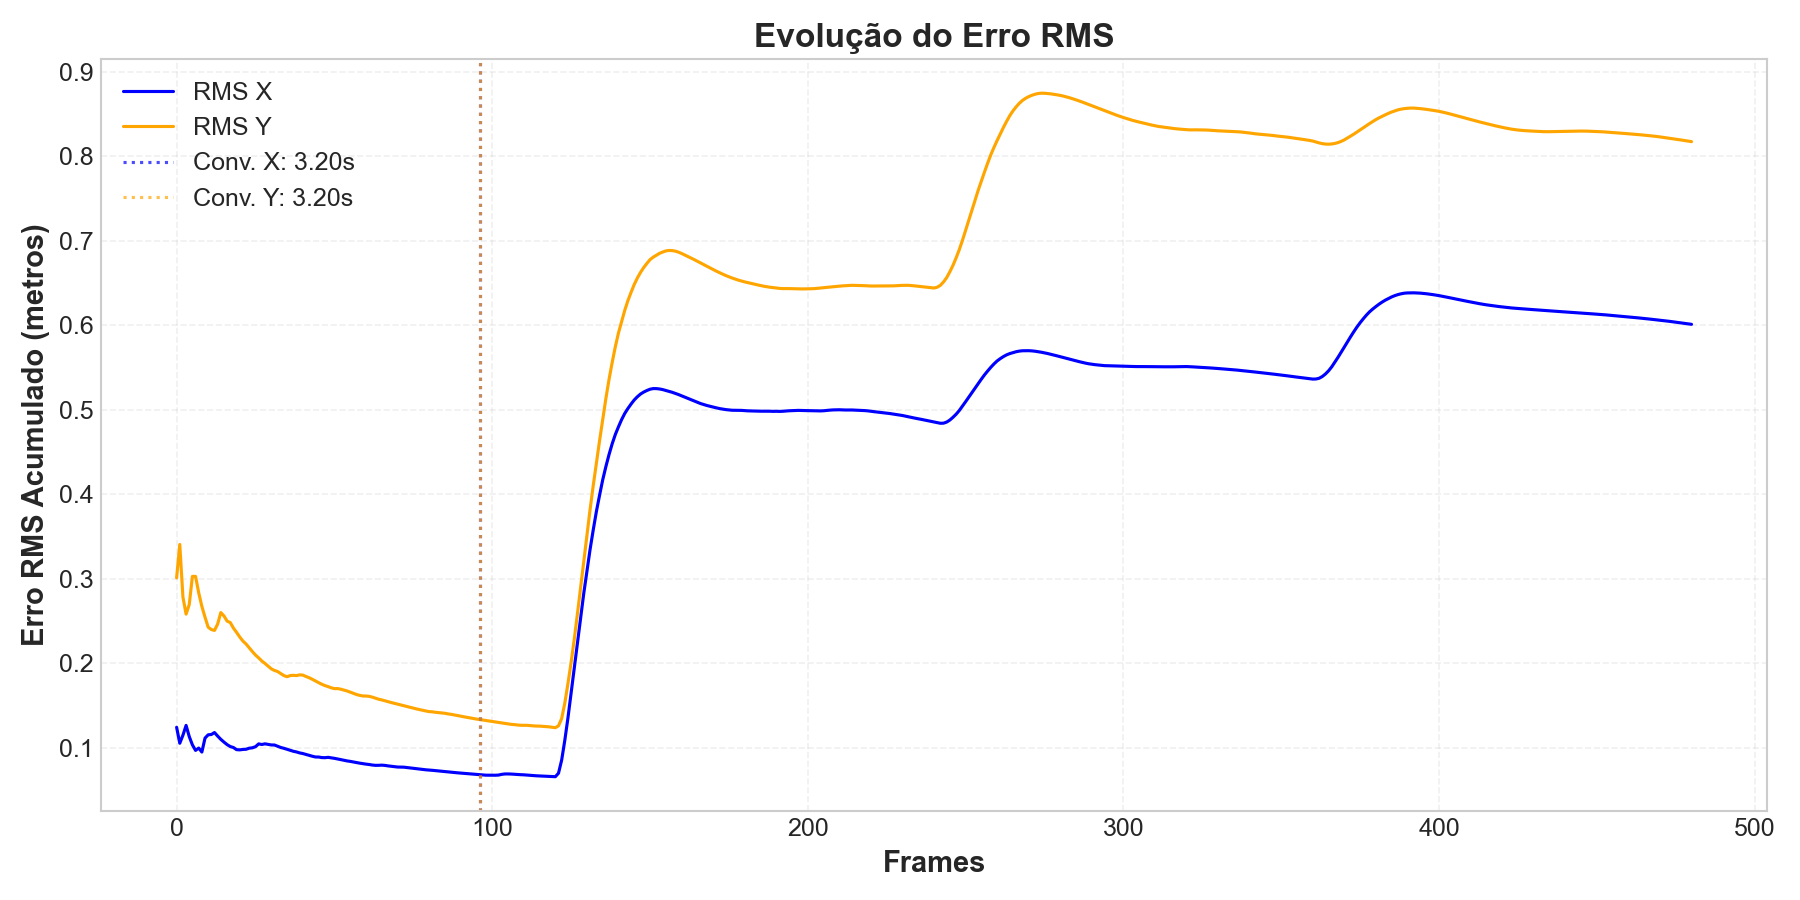
\includegraphics[width=\linewidth]{Figuras/C2/nsintonizado/simulacao_quadrado_2_rms.png}
        \vspace{1mm} \par {\small (b) Quadrado}
    \end{minipage}
    \hfill
    \begin{minipage}[b]{0.32\linewidth}
        \centering
        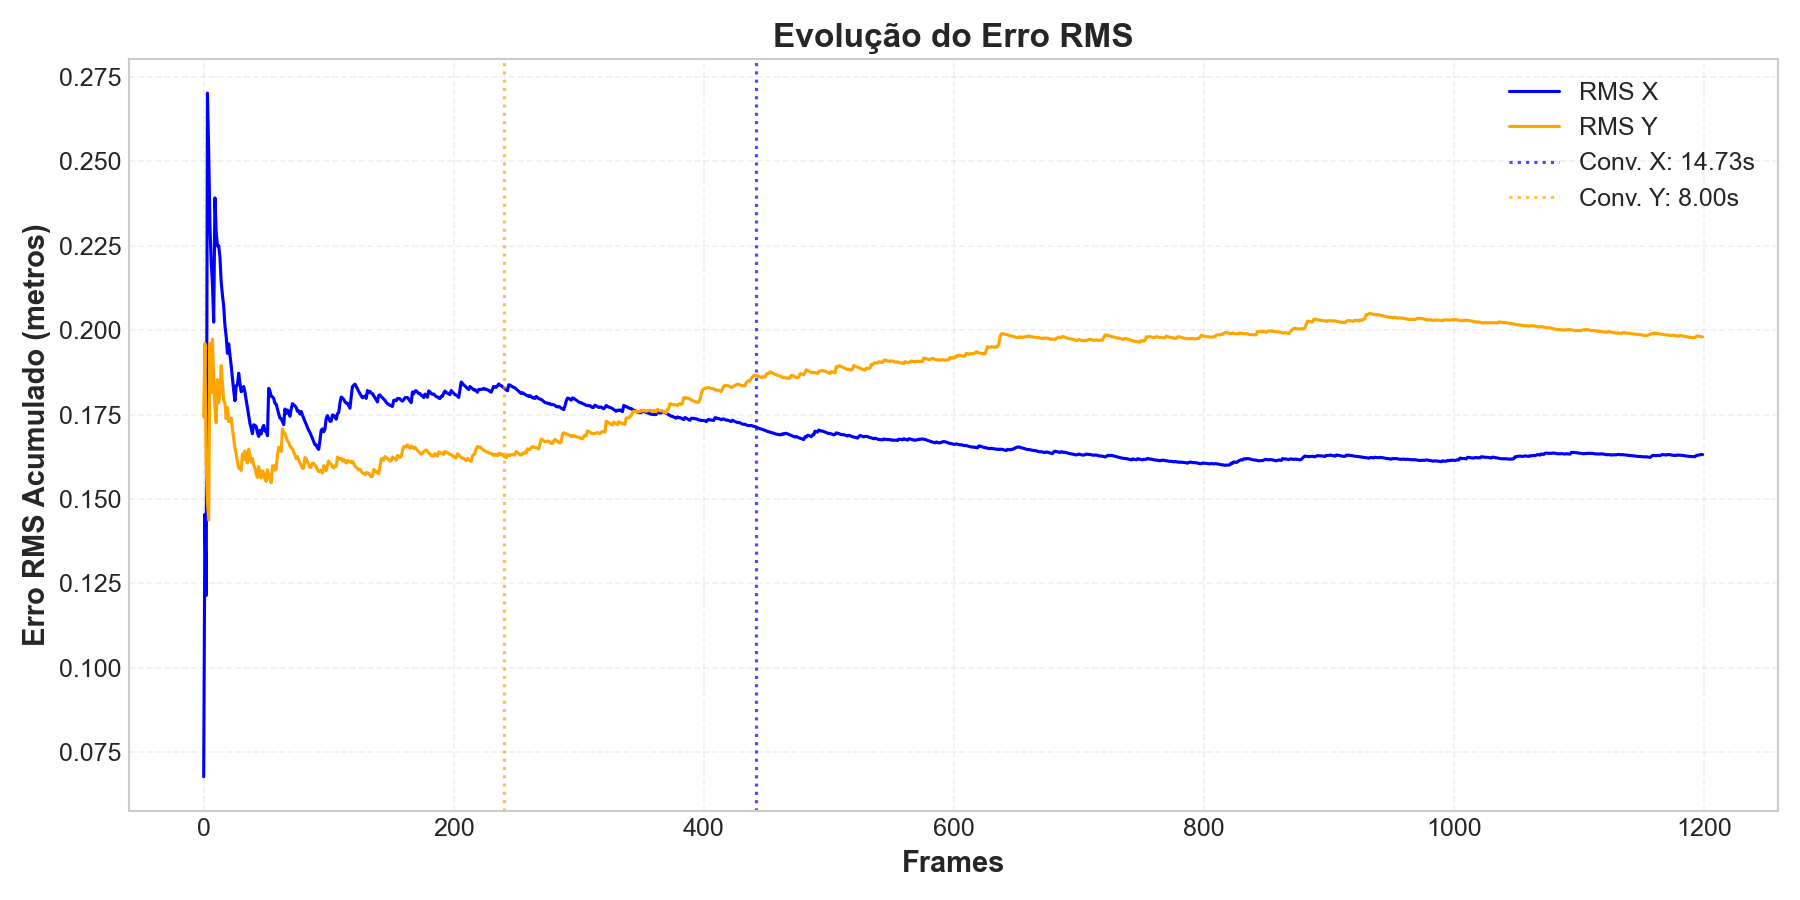
\includegraphics[width=\linewidth]{Figuras/C3/nsintonizado/simulacao_tangente_hiperbólica_2_rms.png}
        \vspace{1mm} \par {\small (c) Tangente Hiperbólica}
    \end{minipage}
    
    \vspace{3mm}
    
    % Linha 2
    \begin{minipage}[b]{0.32\linewidth}
        \centering
        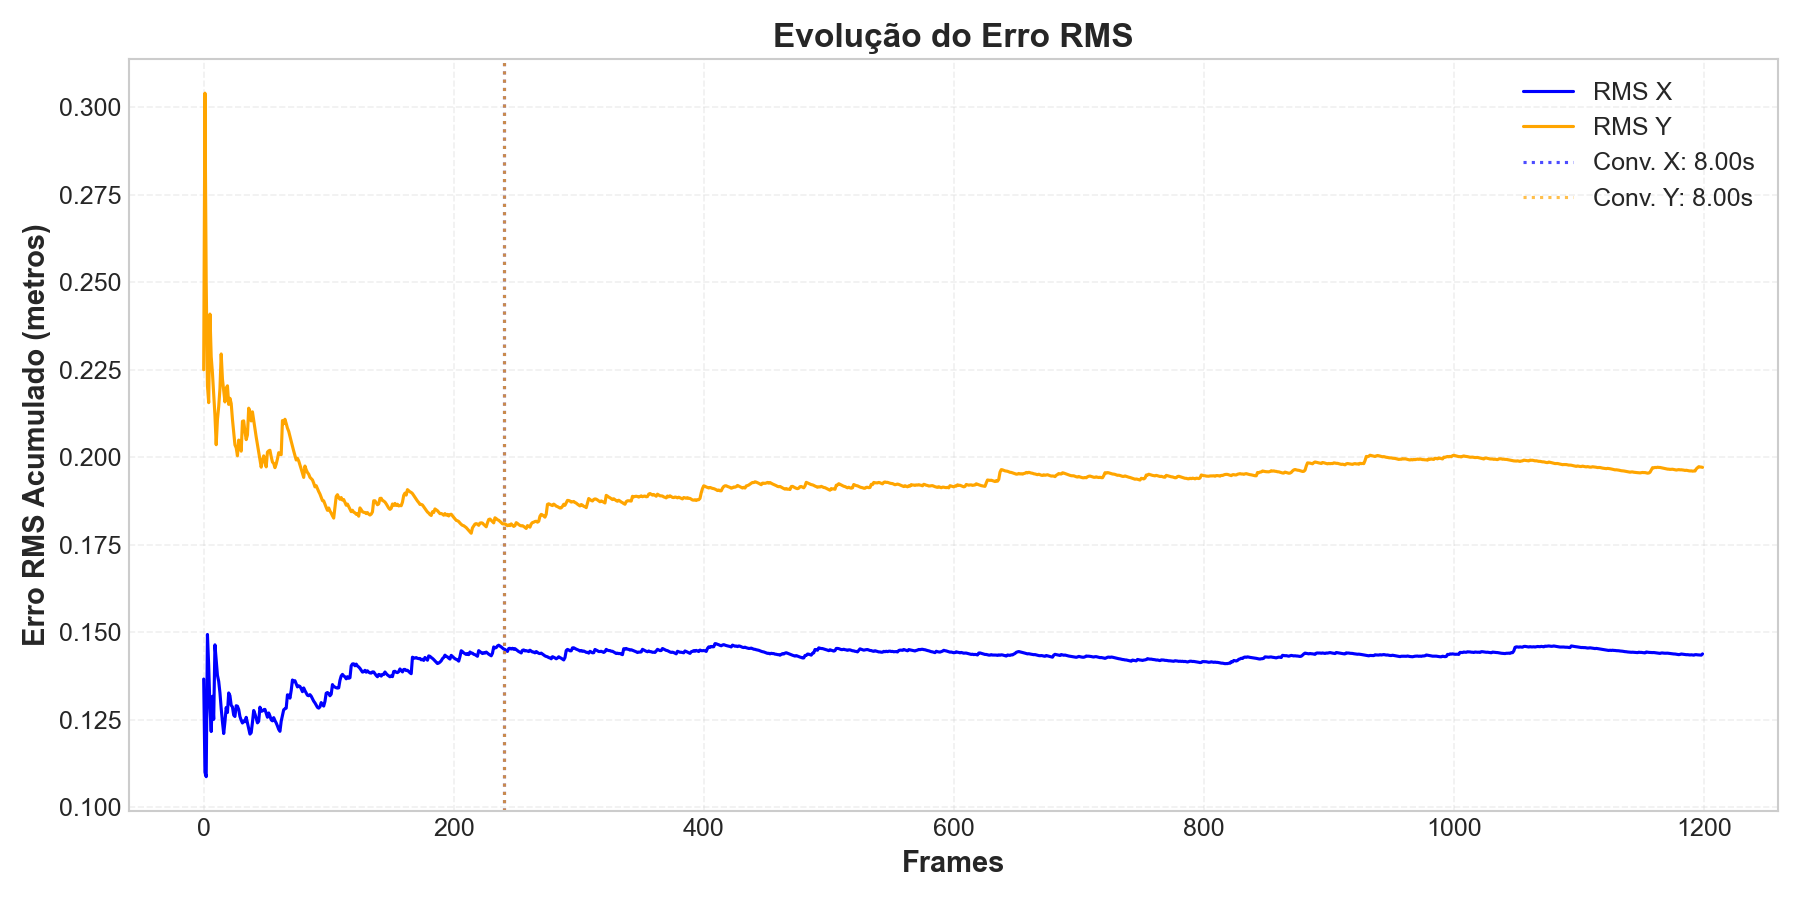
\includegraphics[width=\linewidth]{Figuras/C4/nsintonizado/simulacao_lemniscata_2_rms.png}
        \vspace{1mm} \par {\small (d) Lemniscata}
    \end{minipage}
    \hfill
    \begin{minipage}[b]{0.32\linewidth}
        \centering
        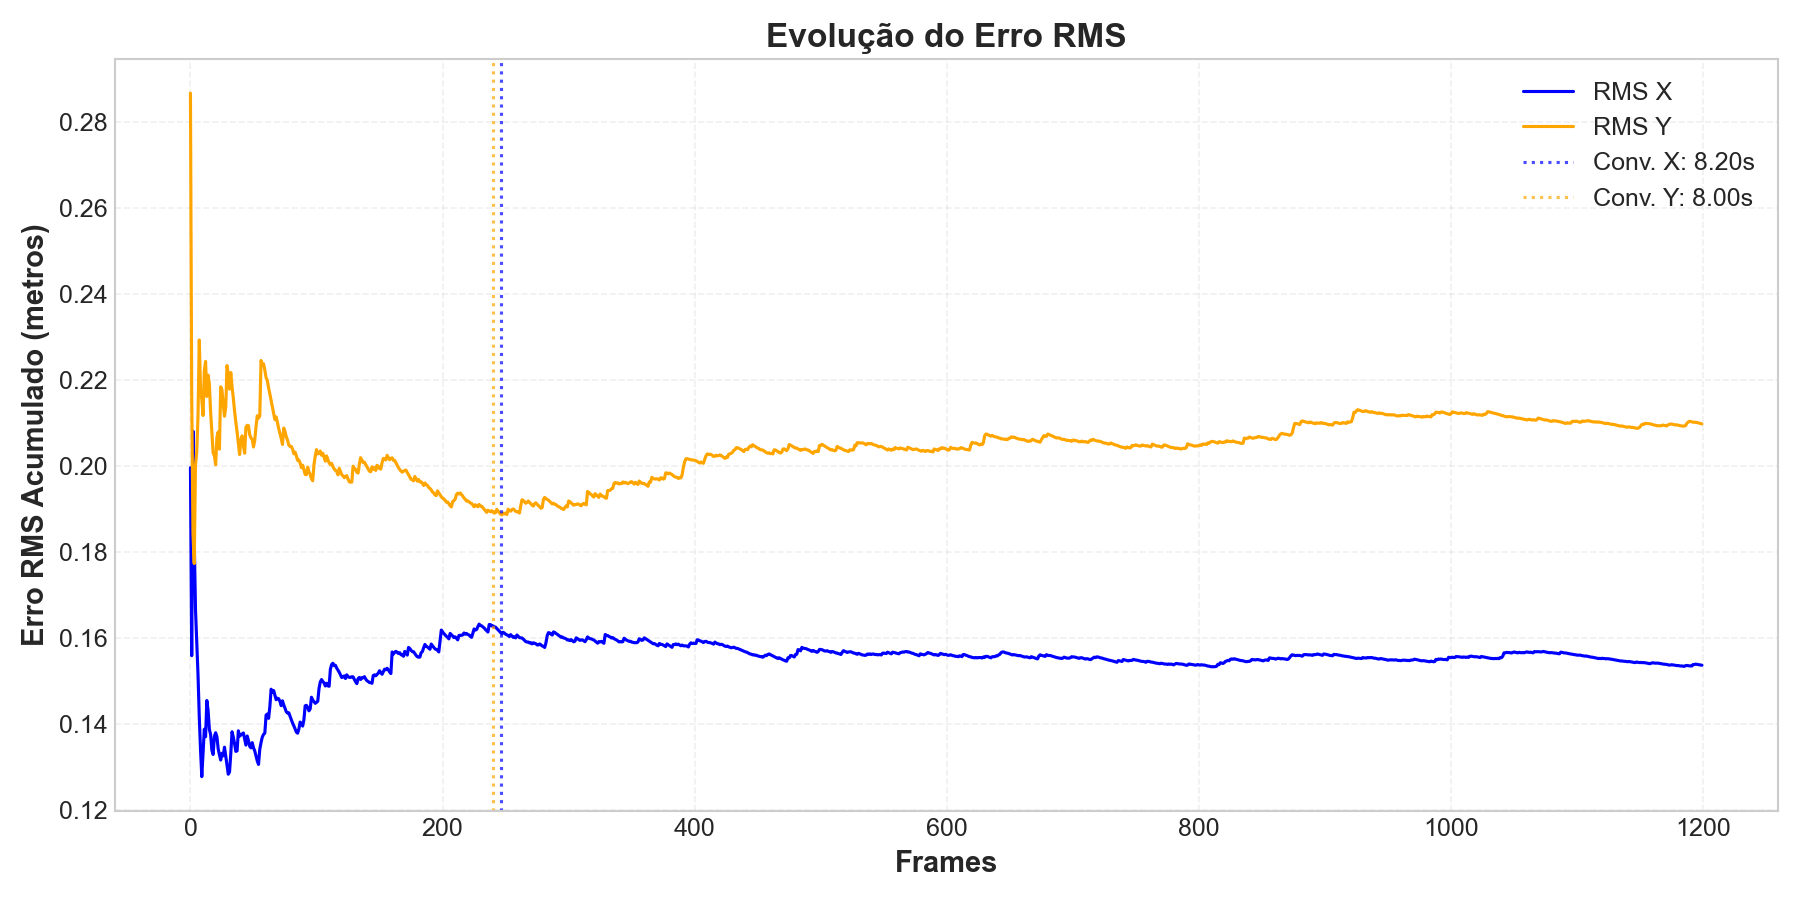
\includegraphics[width=\linewidth]{Figuras/C5/nsintonizado/simulacao_aleatória_2_rms.png}
        \vspace{1mm} \par {\small (e) Aleatória}
    \end{minipage}
    \hfill
    \begin{minipage}[b]{0.32\linewidth}
        \centering
        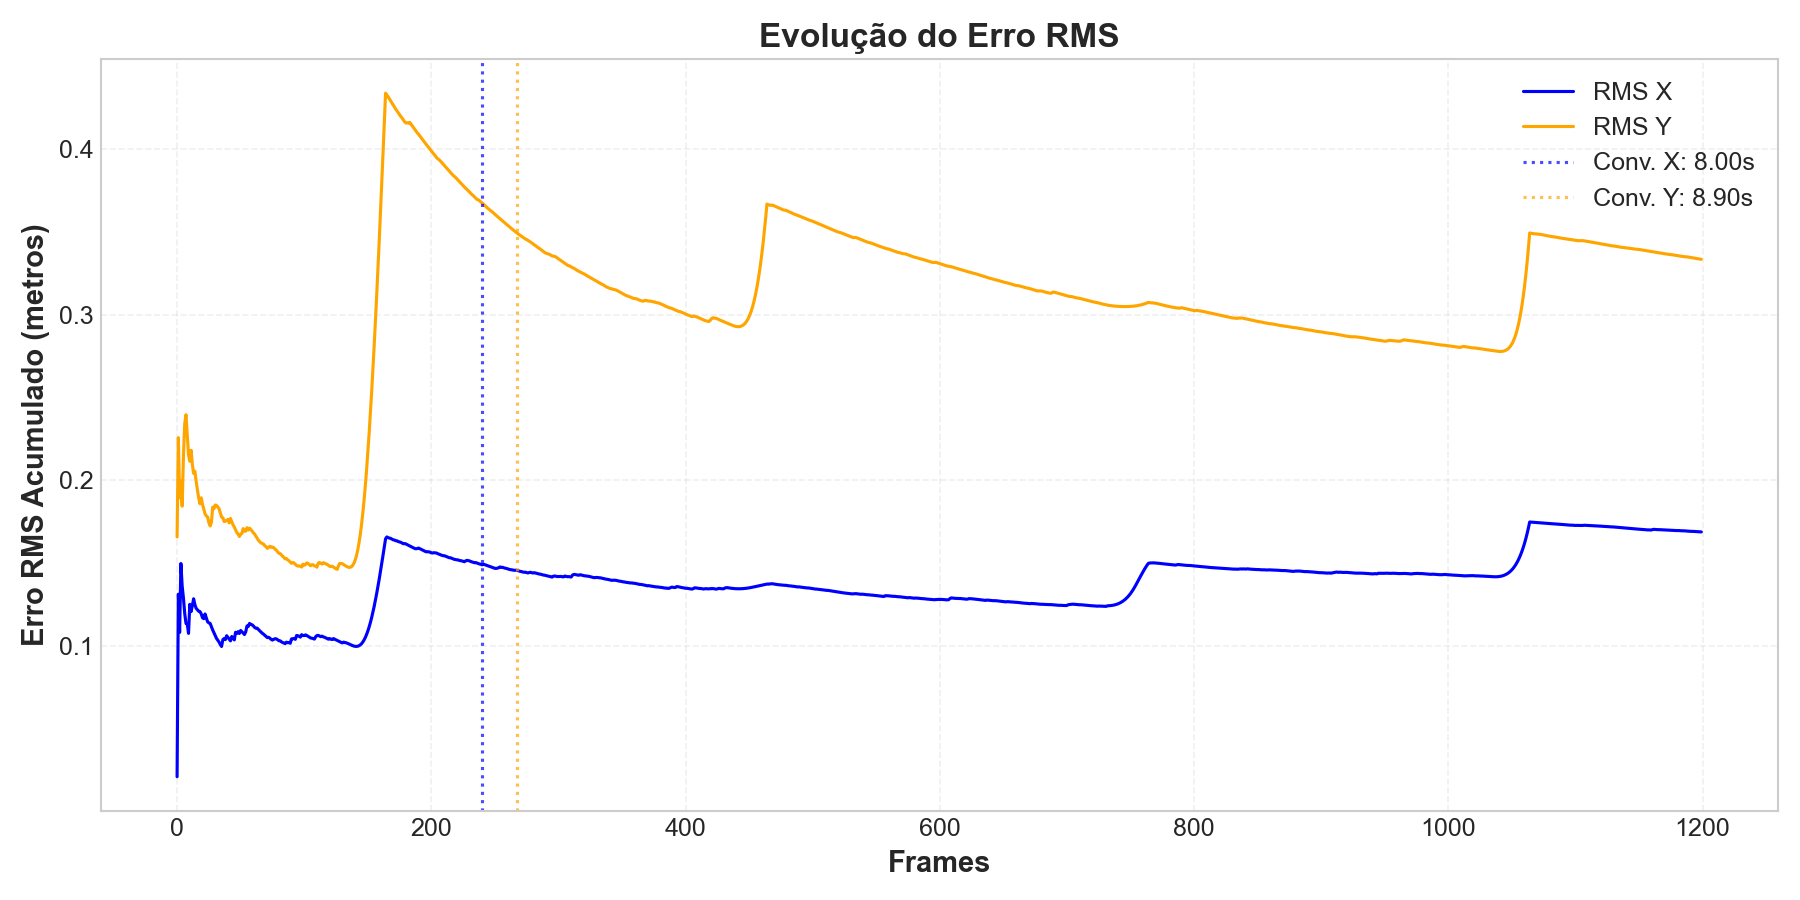
\includegraphics[width=\linewidth]{Figuras/C6/nsintonizado/simulacao_oclusão_2_rms.png}
        \vspace{1mm} \par {\small (f) Oclusão}
    \end{minipage}
    
    \caption{Evolução temporal da métrica RMSE para a \textbf{condição não sintonizada}.}
    \label{fig:app_rmse_naosintonizado_grid}
\end{figure*}

% QUEBRA DE PÁGINA OBRIGATÓRIA
\clearpage

% ==============================================================
% PÁGINA 3: TODOS OS GRÁFICOS NIS (SINTONIZADOS E NÃO SINTONIZADOS) - MAIORES
% ==============================================================
\begin{figure*}[!htpb]
    \centering
    
    % --- PARTE A: NIS SINTONIZADO ---
    % Linha 1
    \begin{minipage}[b]{0.32\linewidth}
        \centering
        
\includegraphics[width=\linewidth]{Figuras/C1/sintonizado/simulacao_círculo_4_nis.png}
        \vspace{1mm} \par {\small (a) Círculo}
    \end{minipage}
    \hfill
    \begin{minipage}[b]{0.32\linewidth}
        \centering
        
\includegraphics[width=\linewidth]{Figuras/C2/sintonizado/simulacao_quadrado_4_nis.png}
        \vspace{1mm} \par {\small (b) Quadrado}
    \end{minipage}
    \hfill
    \begin{minipage}[b]{0.32\linewidth}
        \centering
        
\includegraphics[width=\linewidth]{Figuras/C3/sintonizado/simulacao_tangente_hiperbólica_4_nis.png}
        \vspace{1mm} \par {\small (c) Tangente Hiperbólica}
    \end{minipage}
    
    \vspace{3mm}
    
    % Linha 2
    \begin{minipage}[b]{0.32\linewidth}
        \centering
        
\includegraphics[width=\linewidth]{Figuras/C4/sintonizado/simulacao_lemniscata_4_nis.png}
        \vspace{1mm} \par {\small (d) Lemniscata}
    \end{minipage}
    \hfill
    \begin{minipage}[b]{0.32\linewidth}
        \centering
        
\includegraphics[width=\linewidth]{Figuras/C5/sintonizado/simulacao_aleatória_4_nis.png}
        \vspace{1mm} \par {\small (e) Aleatória}
    \end{minipage}
    \hfill
    \begin{minipage}[b]{0.32\linewidth}
        \centering
        
\includegraphics[width=\linewidth]{Figuras/C6/sintonizado/simulacao_oclusão_4_nis.png}
        \vspace{1mm} \par {\small (f) Oclusão}
    \end{minipage}
    
    \caption{Evolução temporal da métrica NIS para a \textbf{condição sintonizada}. A estatística mantém-se predominantemente abaixo do limite de confiança de $95\%$ (linha tracejada em $9,49$), comprovando a consistência interna do estimador.}
    \label{fig:app_nis_sintonizado_grid}

    \vspace{8mm} % ESPAÇO ENTRE OS DOIS BLOCOS DE NIS

    % --- PARTE B: NIS NÃO SINTONIZADO ---
    % Linha 1
    \begin{minipage}[b]{0.32\linewidth}
        \centering
        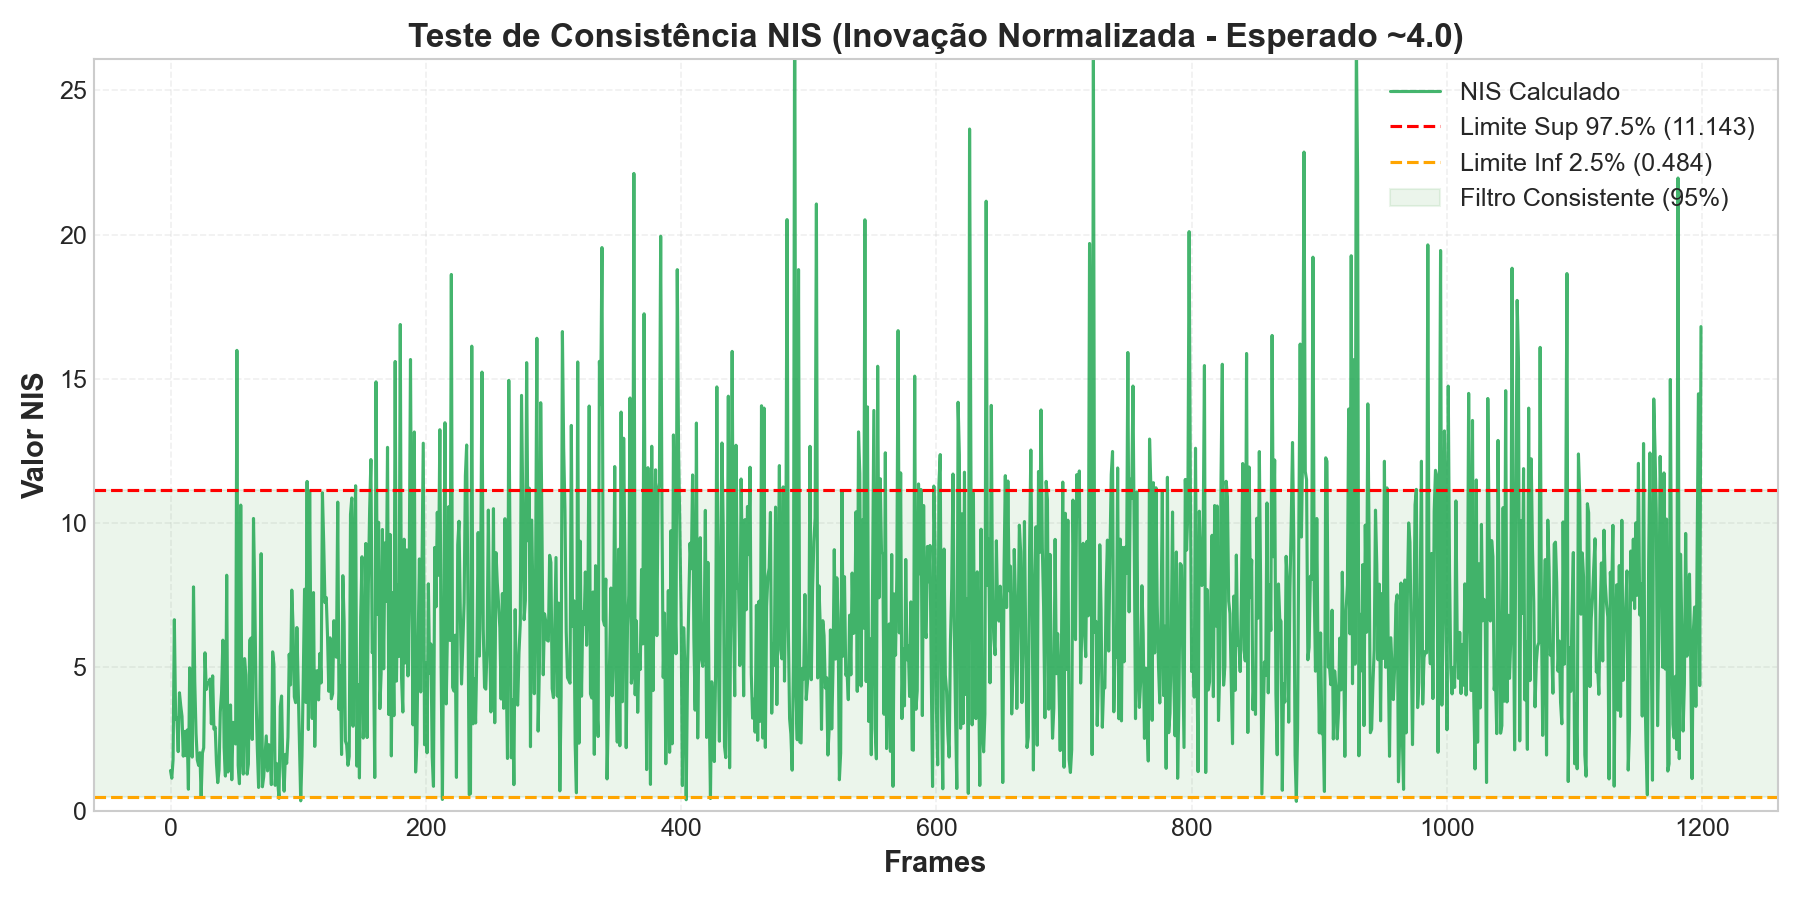
\includegraphics[width=\linewidth]{Figuras/C1/nsintonizado/simulacao_círculo_4_nis.png}
        \vspace{1mm} \par {\small (a) Círculo}
    \end{minipage}
    \hfill
    \begin{minipage}[b]{0.32\linewidth}
        \centering
        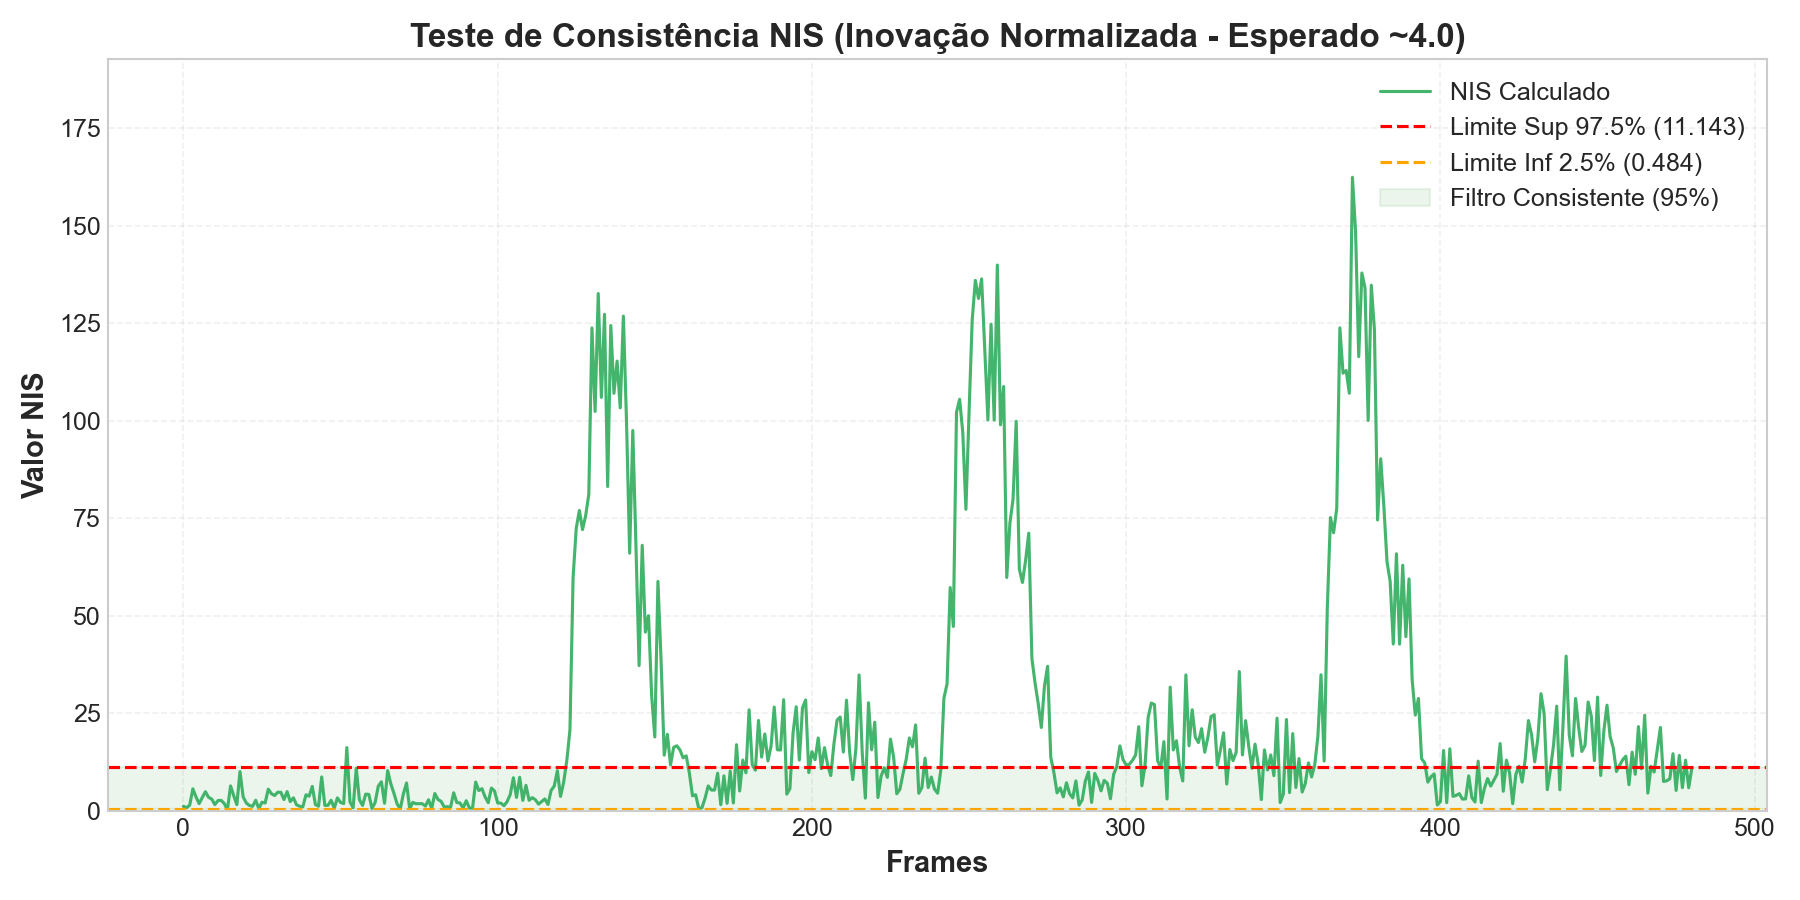
\includegraphics[width=\linewidth]{Figuras/C2/nsintonizado/simulacao_quadrado_4_nis.png}
        \vspace{1mm} \par {\small (b) Quadrado}
    \end{minipage}
    \hfill
    \begin{minipage}[b]{0.32\linewidth}
        \centering
        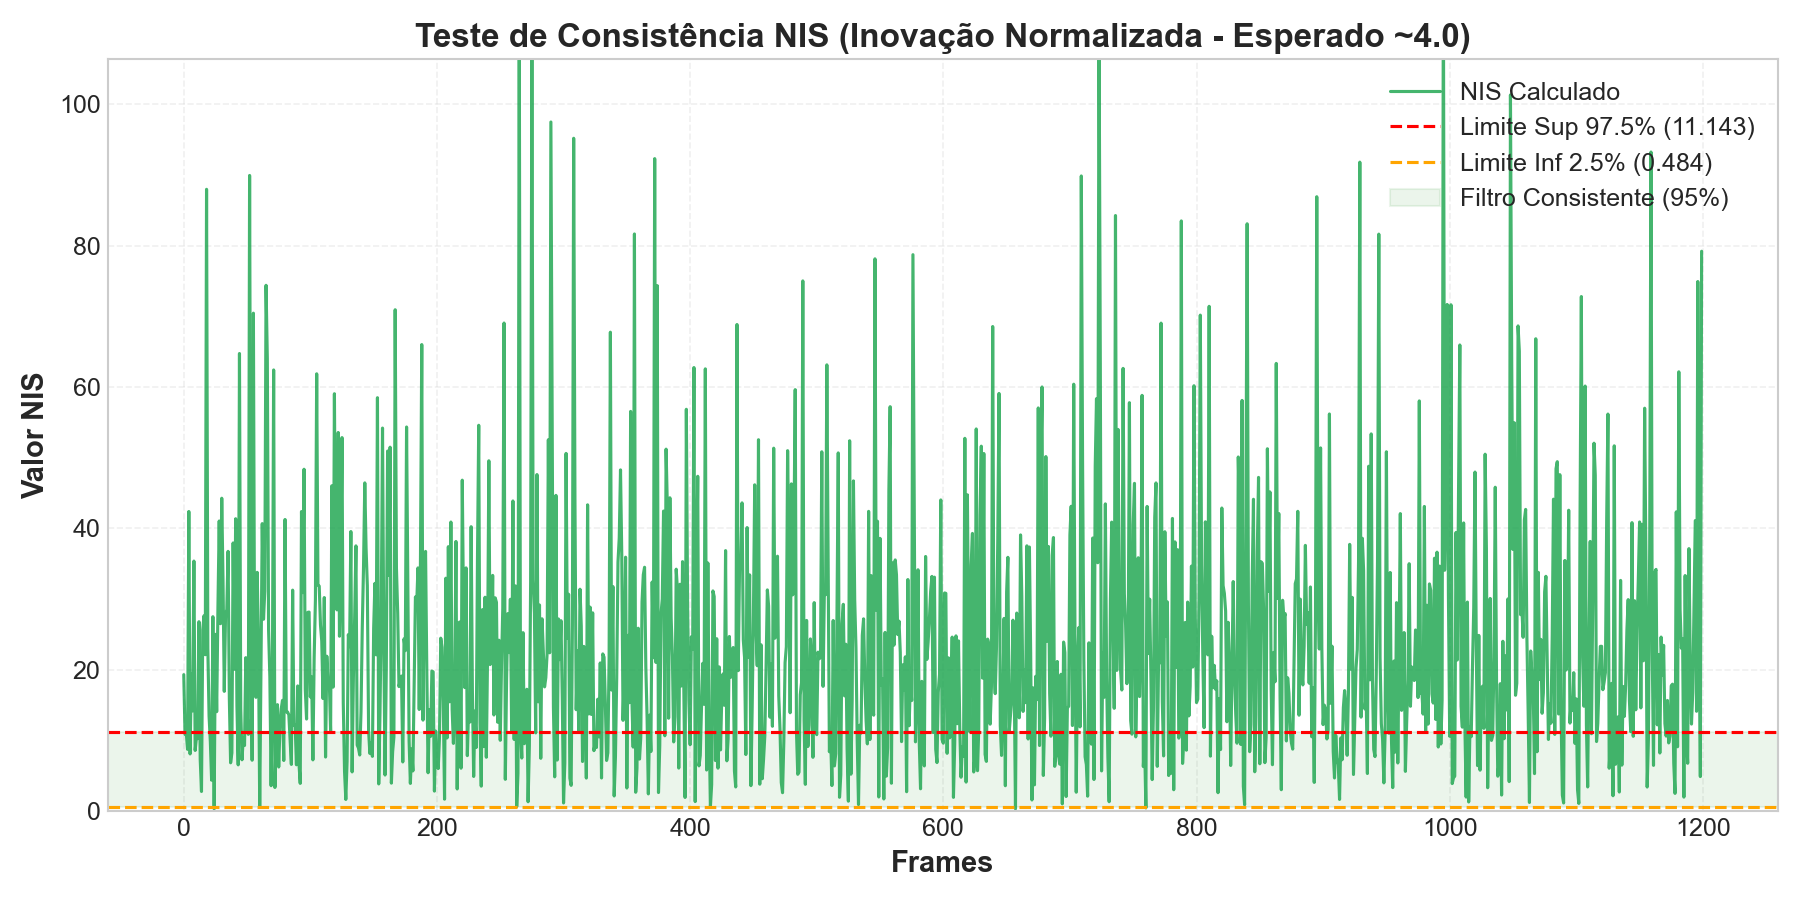
\includegraphics[width=\linewidth]{Figuras/C3/nsintonizado/simulacao_tangente_hiperbólica_4_nis.png}
        \vspace{1mm} \par {\small (c) Tangente Hiperbólica}
    \end{minipage}
    
    \vspace{3mm}
    
    % Linha 2
    \begin{minipage}[b]{0.32\linewidth}
        \centering
        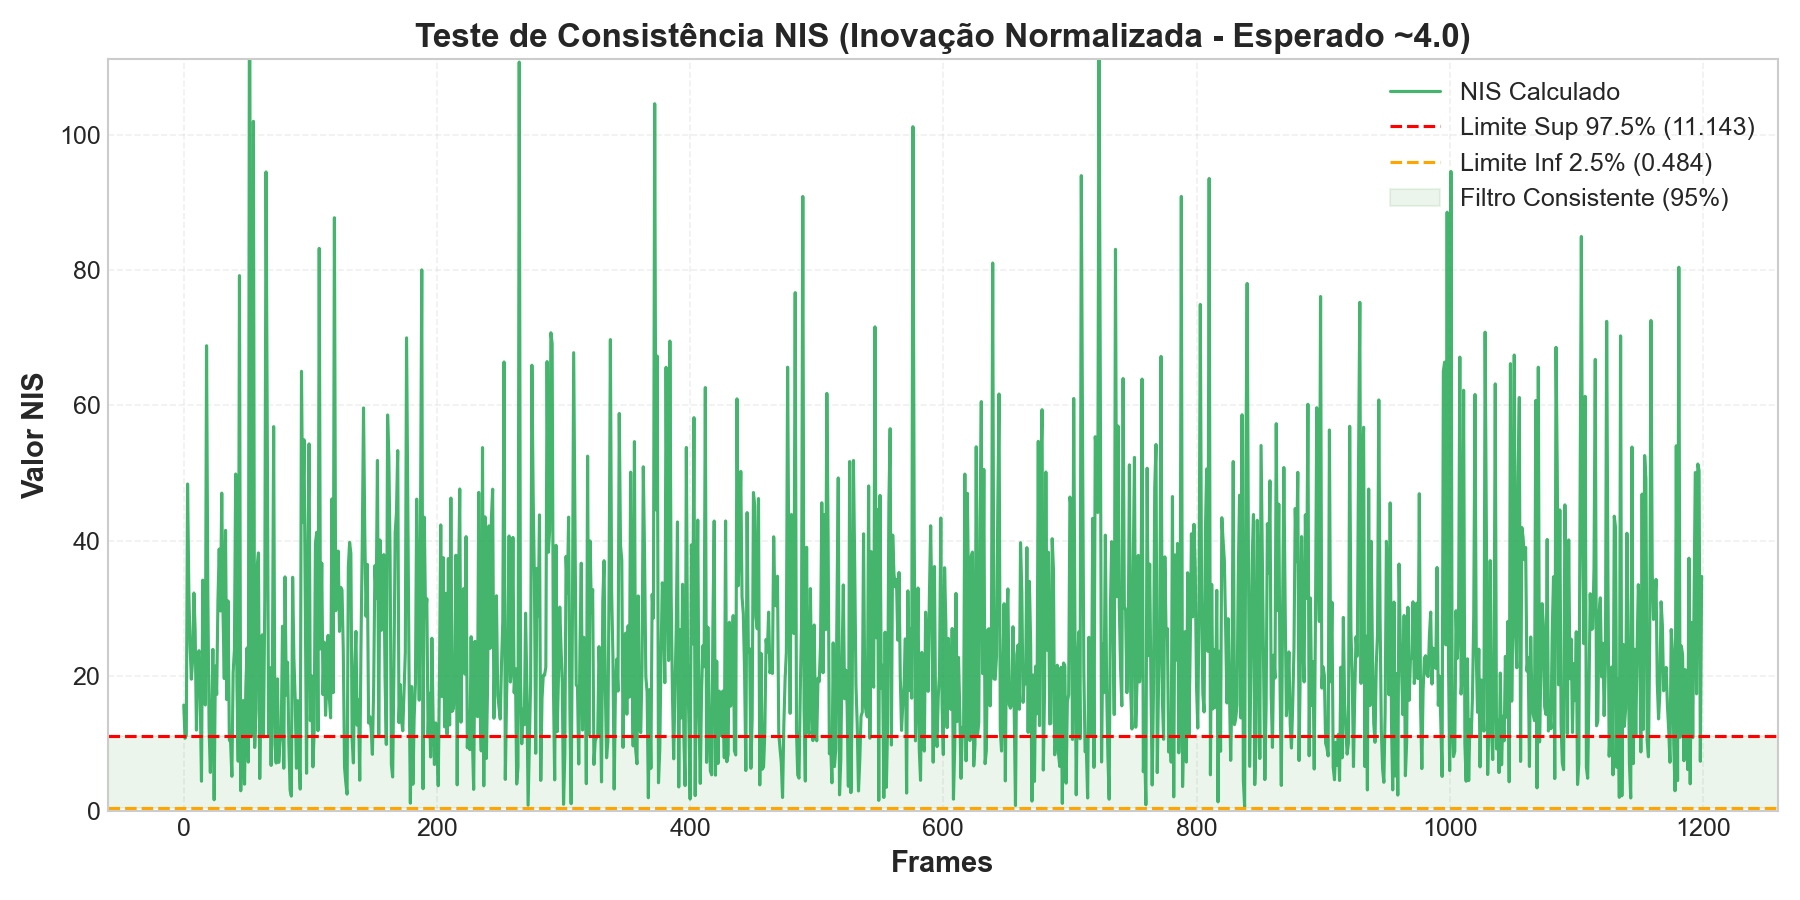
\includegraphics[width=\linewidth]{Figuras/C4/nsintonizado/simulacao_lemniscata_4_nis.png}
        \vspace{1mm} \par {\small (d) Lemniscata}
    \end{minipage}
    \hfill
    \begin{minipage}[b]{0.32\linewidth}
        \centering
        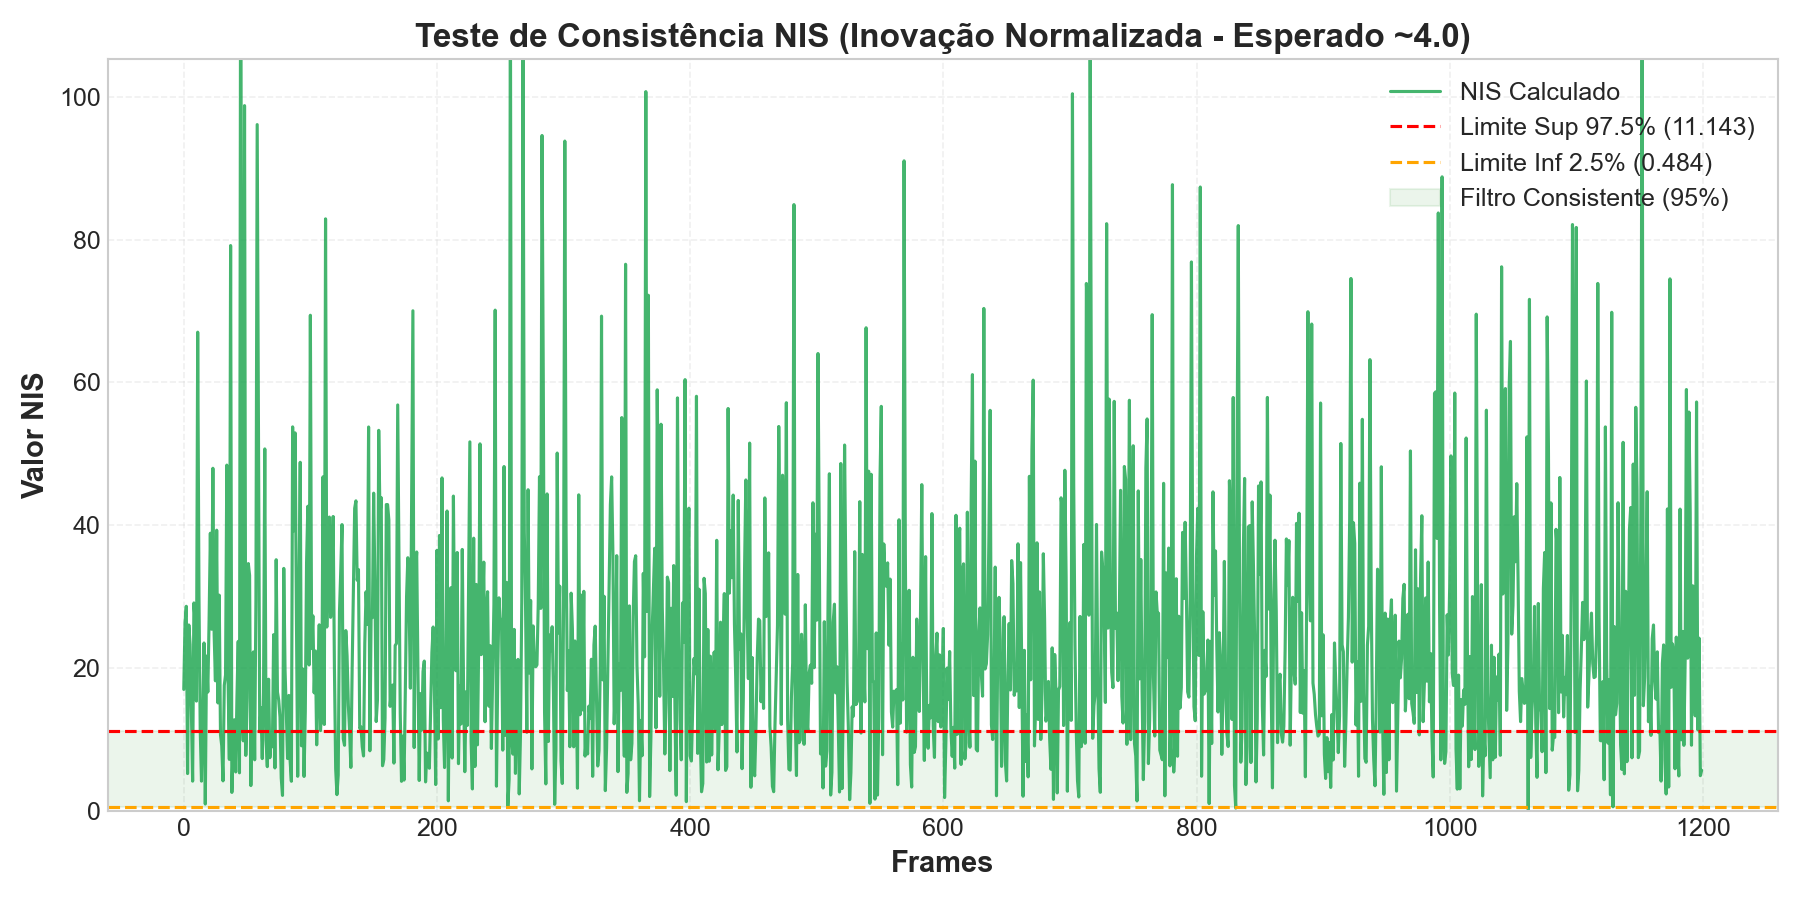
\includegraphics[width=\linewidth]{Figuras/C5/nsintonizado/simulacao_aleatória_4_nis.png}
        \vspace{1mm} \par {\small (e) Aleatória}
    \end{minipage}
    \hfill
    \begin{minipage}[b]{0.32\linewidth}
        \centering
        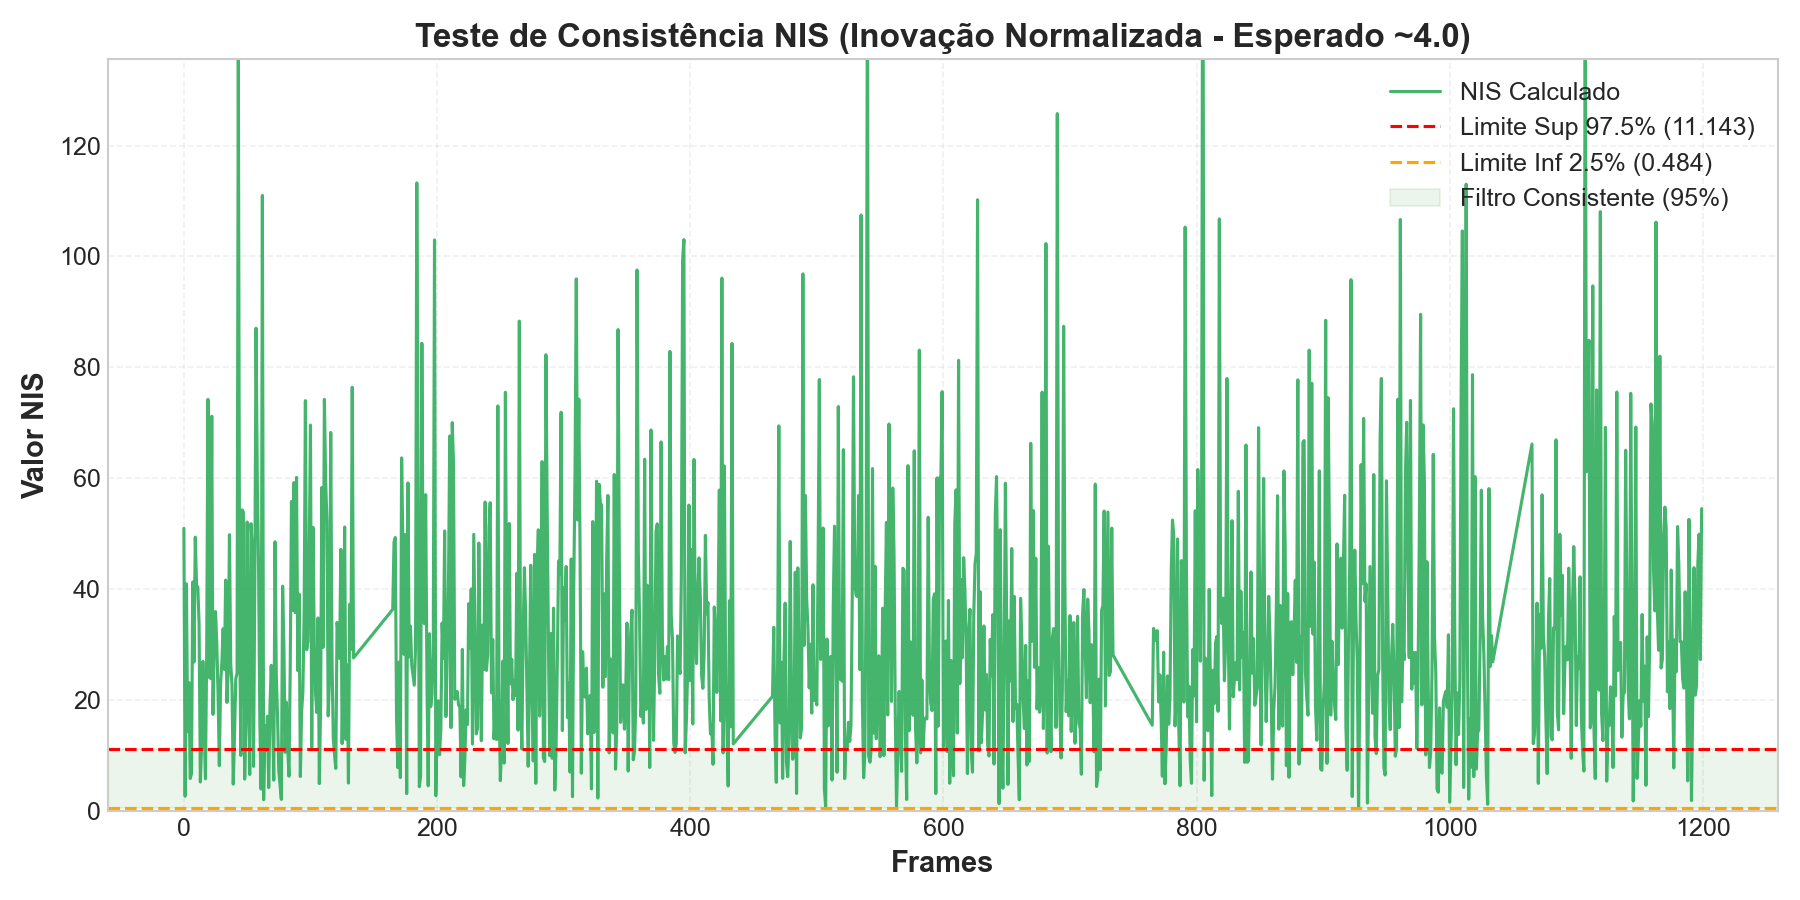
\includegraphics[width=\linewidth]{Figuras/C6/nsintonizado/simulacao_oclusão_4_nis.png}
        \vspace{1mm} \par {\small (f) Oclusão}
    \end{minipage}
    
    \caption{Evolução temporal da métrica NIS para a \textbf{condição não sintonizada}. A constante violação do limiar estatístico evidencia a degradação estrutural e a perda de confiança na matriz de covariância preditiva.}
    \label{fig:app_nis_naosintonizado_grid}
\end{figure*}

% QUEBRA DE PÁGINA OBRIGATÓRIA
\clearpage

% ==============================================================
% PÁGINA 4: TODOS OS GRÁFICOS HISTOGRAMAS (SINTONIZADOS E NÃO SINTONIZADOS) - MAIORES
% ==============================================================
\begin{figure*}[!htpb]
    \centering
    
    % --- PARTE A: HISTOGRAMA SINTONIZADO ---
    % Linha 1
    \begin{minipage}[b]{0.32\linewidth}
        \centering
        
\includegraphics[width=\linewidth]{Figuras/C1/sintonizado/simulacao_círculo_5_hist.png}
        \vspace{1mm} \par {\small (a) Círculo}
    \end{minipage}
    \hfill
    \begin{minipage}[b]{0.32\linewidth}
        \centering
        
\includegraphics[width=\linewidth]{Figuras/C2/sintonizado/simulacao_quadrado_5_hist.png}
        \vspace{1mm} \par {\small (b) Quadrado}
    \end{minipage}
    \hfill
    \begin{minipage}[b]{0.32\linewidth}
        \centering
        
\includegraphics[width=\linewidth]{Figuras/C3/sintonizado/simulacao_tangente_hiperbólica_5_hist.png}
        \vspace{1mm} \par {\small (c) Tangente Hiperbólica}
    \end{minipage}
    
    \vspace{3mm}
    
    % Linha 2
    \begin{minipage}[b]{0.32\linewidth}
        \centering
        
\includegraphics[width=\linewidth]{Figuras/C4/sintonizado/simulacao_lemniscata_5_hist.png}
        \vspace{1mm} \par {\small (d) Lemniscata}
    \end{minipage}
    \hfill
    \begin{minipage}[b]{0.32\linewidth}
        \centering
        
\includegraphics[width=\linewidth]{Figuras/C5/sintonizado/simulacao_aleatória_5_hist.png}
        \vspace{1mm} \par {\small (e) Aleatória}
    \end{minipage}
    \hfill
    \begin{minipage}[b]{0.32\linewidth}
        \centering
        
\includegraphics[width=\linewidth]{Figuras/C6/sintonizado/simulacao_oclusão_5_hist.png}
        \vspace{1mm} \par {\small (f) Oclusão}
    \end{minipage}
    
    \caption{Distribuição dos resíduos (histogramas) para a \textbf{condição sintonizada}. Os perfis mantêm forte aderência à distribuição normal, indicando que as inovações do filtro são não viesadas.}
    \label{fig:app_hist_sintonizado_grid}

    \vspace{8mm} % ESPAÇO ENTRE OS DOIS BLOCOS DE HISTOGRAMAS

    % --- PARTE B: HISTOGRAMA NÃO SINTONIZADO ---
    % Linha 1
    \begin{minipage}[b]{0.32\linewidth}
        \centering
        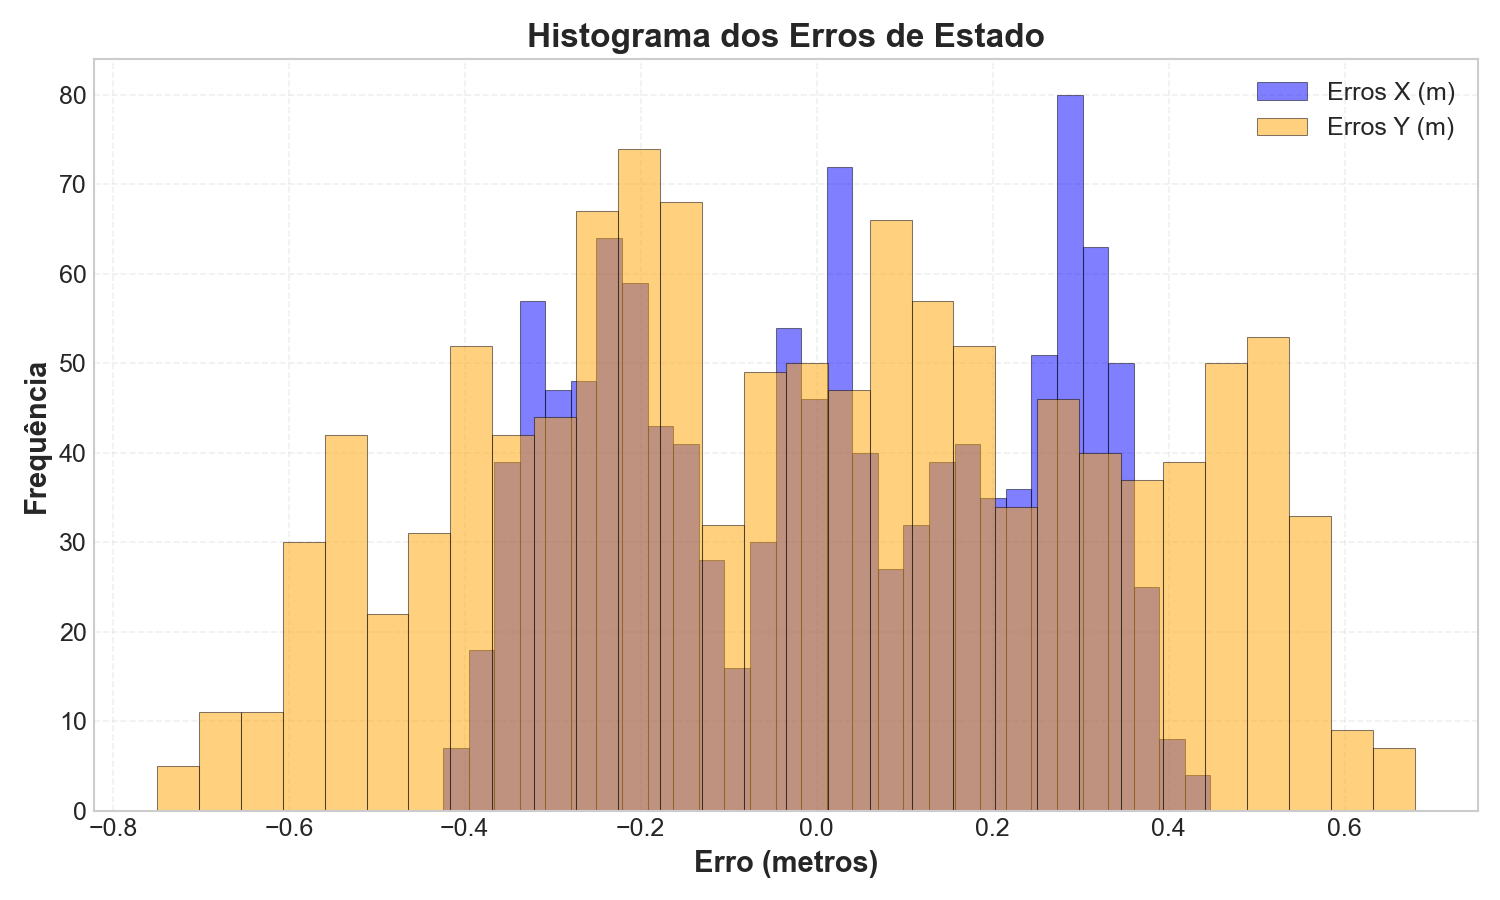
\includegraphics[width=\linewidth]{Figuras/C1/nsintonizado/simulacao_círculo_5_hist.png}
        \vspace{1mm} \par {\small (a) Círculo}
    \end{minipage}
    \hfill
    \begin{minipage}[b]{0.32\linewidth}
        \centering
        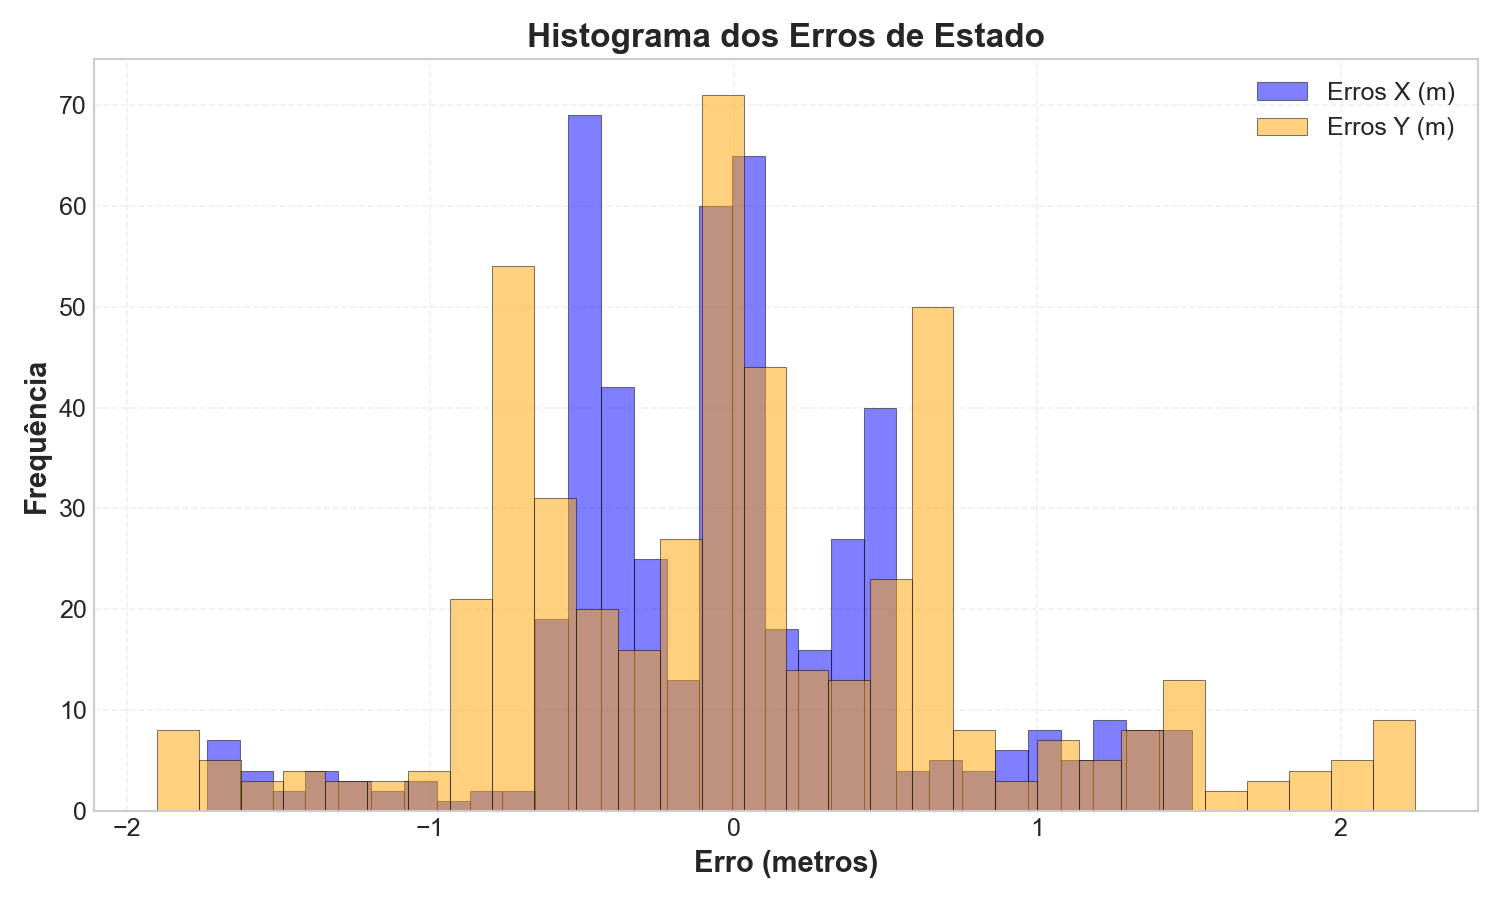
\includegraphics[width=\linewidth]{Figuras/C2/nsintonizado/simulacao_quadrado_5_hist.png}
        \vspace{1mm} \par {\small (b) Quadrado}
    \end{minipage}
    \hfill
    \begin{minipage}[b]{0.32\linewidth}
        \centering
        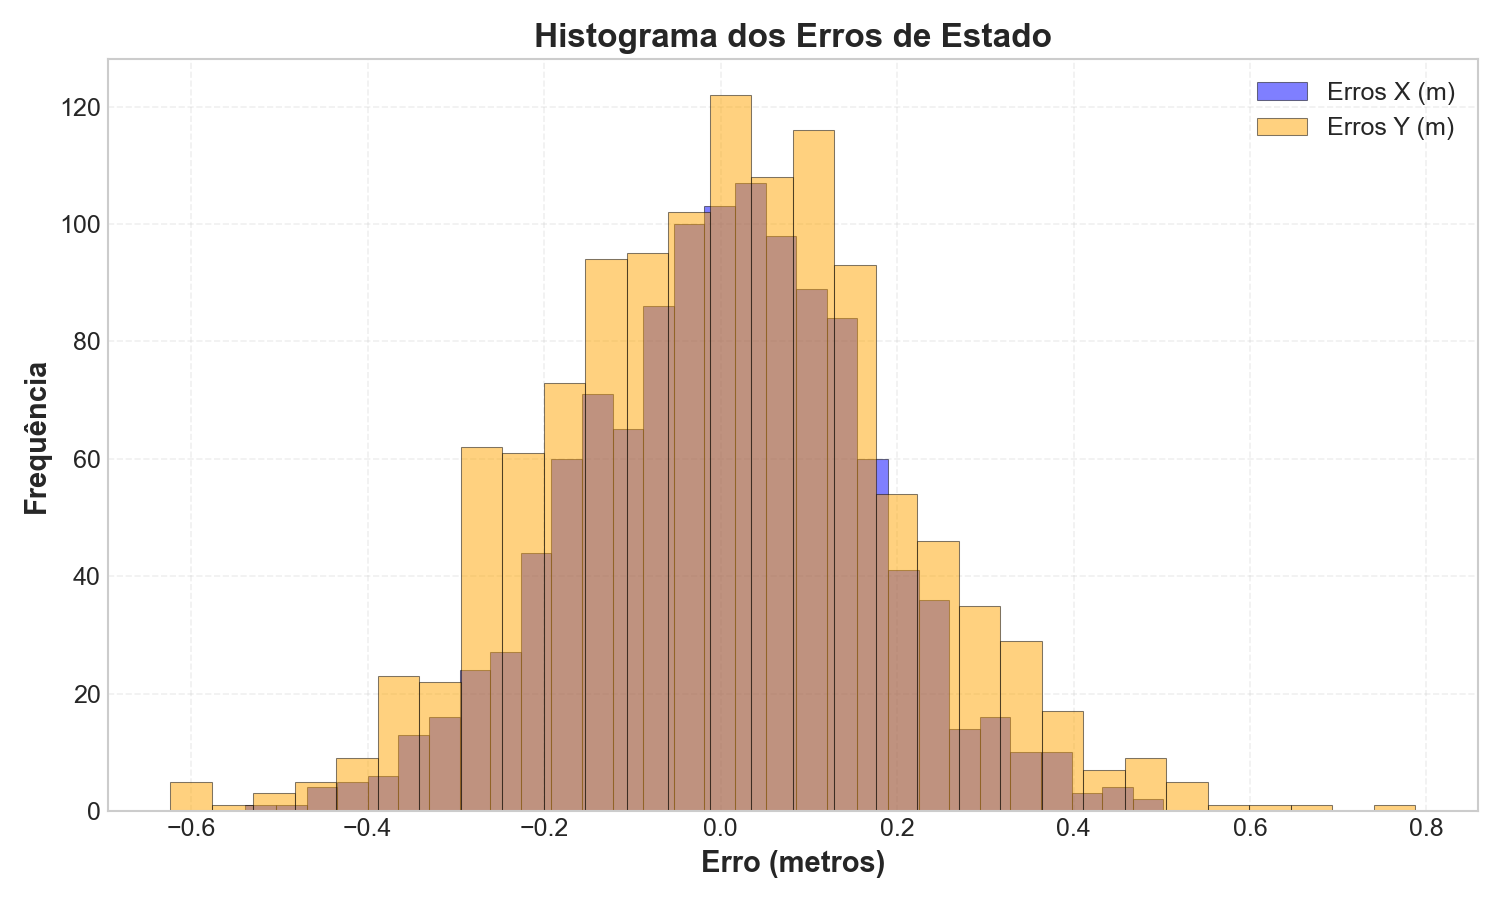
\includegraphics[width=\linewidth]{Figuras/C3/nsintonizado/simulacao_tangente_hiperbólica_5_hist.png}
        \vspace{1mm} \par {\small (c) Tangente Hiperbólica}
    \end{minipage}
    
    \vspace{3mm}
    
    % Linha 2
    \begin{minipage}[b]{0.32\linewidth}
        \centering
        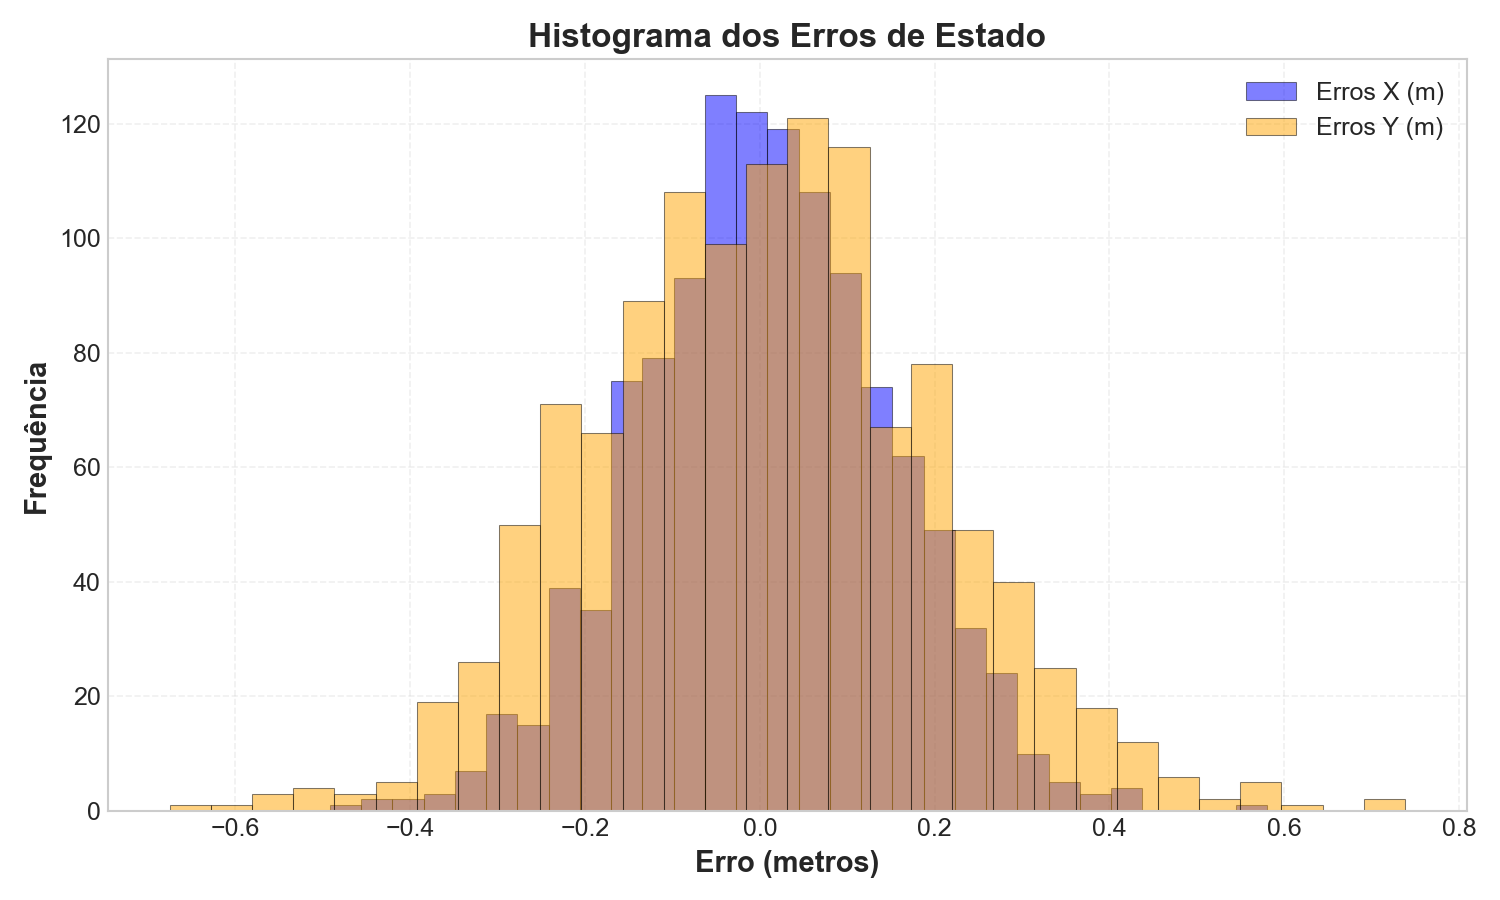
\includegraphics[width=\linewidth]{Figuras/C4/nsintonizado/simulacao_lemniscata_5_hist.png}
        \vspace{1mm} \par {\small (d) Lemniscata}
    \end{minipage}
    \hfill
    \begin{minipage}[b]{0.32\linewidth}
        \centering
        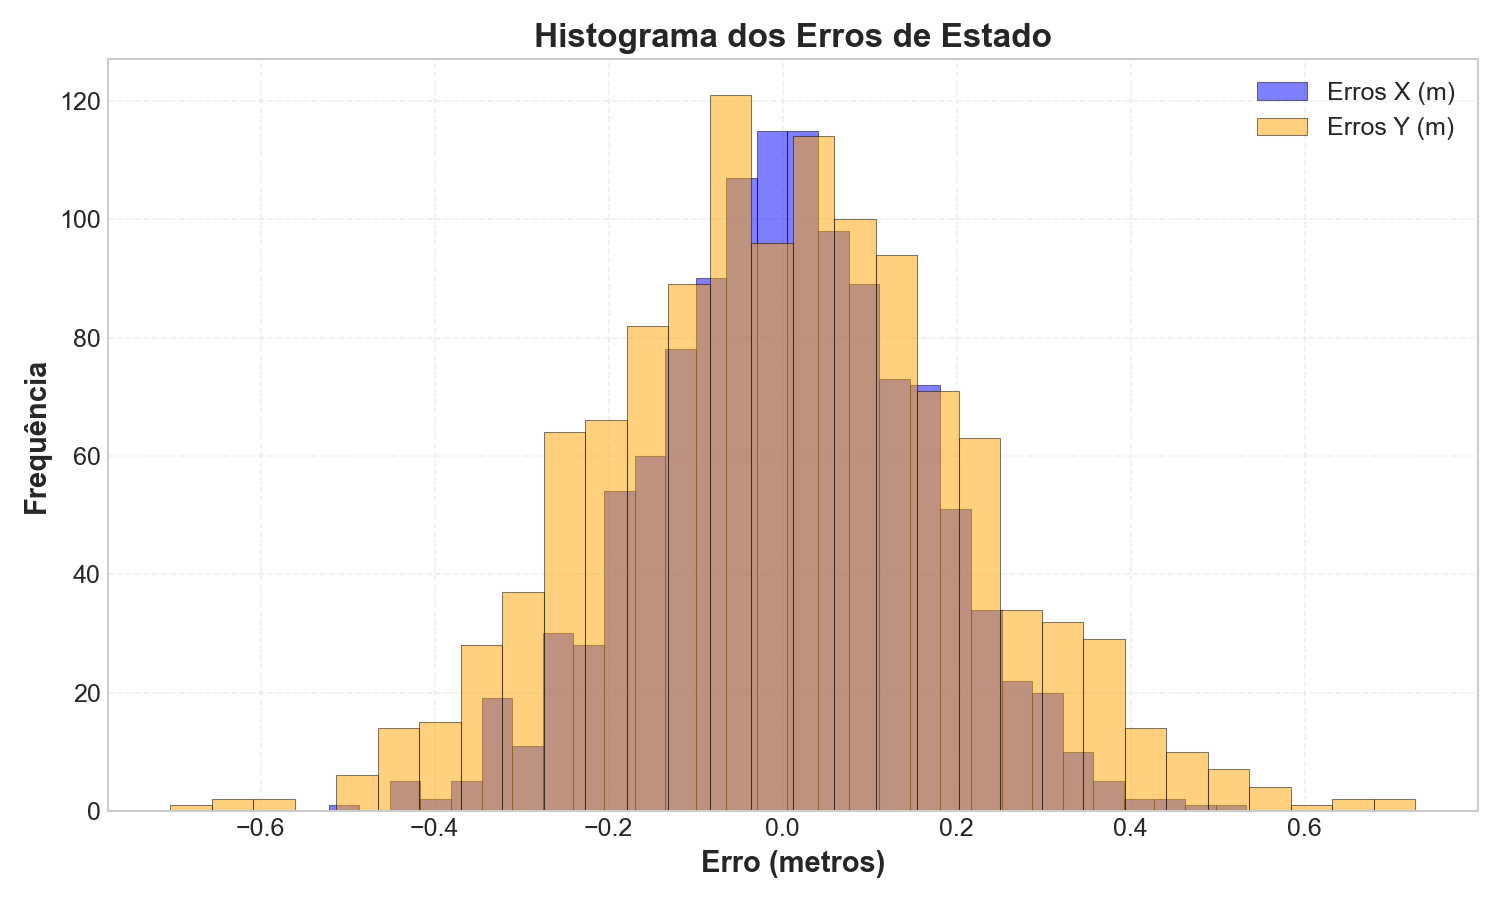
\includegraphics[width=\linewidth]{Figuras/C5/nsintonizado/simulacao_aleatória_5_hist.png}
        \vspace{1mm} \par {\small (e) Aleatória}
    \end{minipage}
    \hfill
    \begin{minipage}[b]{0.32\linewidth}
        \centering
        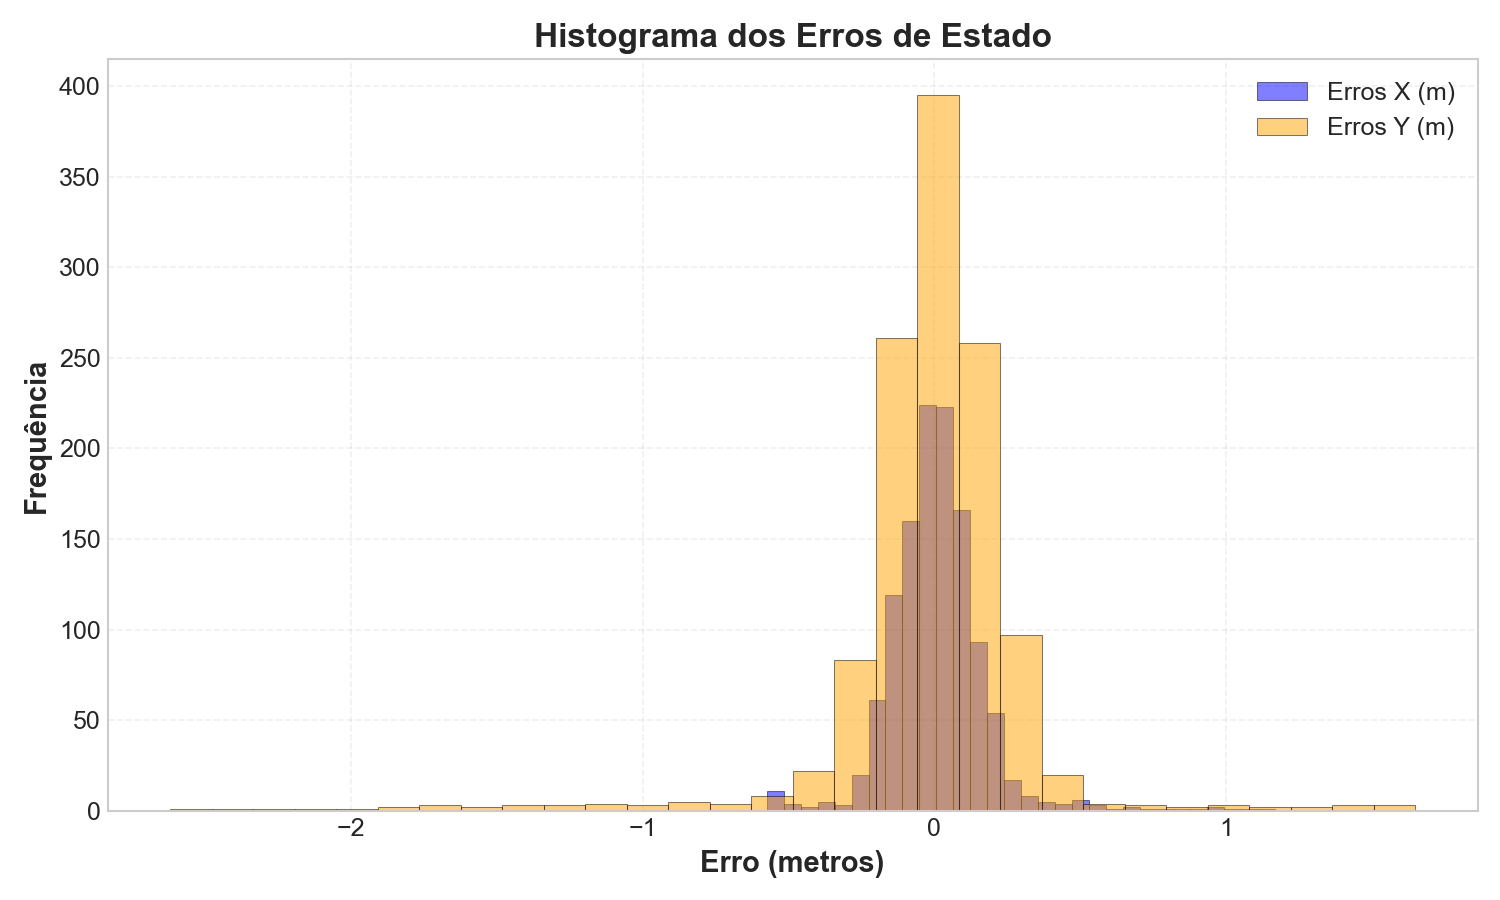
\includegraphics[width=\linewidth]{Figuras/C6/nsintonizado/simulacao_oclusão_5_hist.png}
        \vspace{1mm} \par {\small (f) Oclusão}
    \end{minipage}

    \caption{Distribuição dos resíduos (histogramas) para a \textbf{condição não sintonizada}. Observa-se a acentuada perda de normalidade e o surgimento de assimetrias, o que caracteriza um comportamento subótimo.}
    \label{fig:app_hist_naosintonizado_grid}
\end{figure*}

% QUEBRA DE PÁGINA OBRIGATÓRIA
\clearpage

% ==============================================================
% PÁGINA 5: TODOS OS GRÁFICOS SCATTER (SINTONIZADOS E NÃO SINTONIZADOS) - MAIORES
% ==============================================================
\begin{figure*}[!htpb]
    \centering
    
    % --- PARTE A: SCATTER SINTONIZADO ---
    % Linha 1
    \begin{minipage}[b]{0.24\linewidth}
        \centering
        
\includegraphics[width=\linewidth]{Figuras/C1/sintonizado/simulacao_círculo_3_scatter.png}
        \vspace{1mm} \par {\small (a) Círculo}
    \end{minipage}
    \hfill
    \begin{minipage}[b]{0.24\linewidth}
        \centering
        
\includegraphics[width=\linewidth]{Figuras/C2/sintonizado/simulacao_quadrado_3_scatter.png}
        \vspace{1mm} \par {\small (b) Quadrado}
    \end{minipage}
    \hfill
    \begin{minipage}[b]{0.24\linewidth}
        \centering
        
\includegraphics[width=\linewidth]{Figuras/C3/sintonizado/simulacao_tangente_hiperbólica_3_scatter.png}
        \vspace{1mm} \par {\small (c) Tangente Hiperbólica}
    \end{minipage}
    
    \vspace{3mm}
    
    % Linha 2
    \begin{minipage}[b]{0.24\linewidth}
        \centering
        
\includegraphics[width=\linewidth]{Figuras/C4/sintonizado/simulacao_lemniscata_3_scatter.png}
        \vspace{1mm} \par {\small (d) Lemniscata}
    \end{minipage}
    \hfill
    \begin{minipage}[b]{0.24\linewidth}
        \centering
        
\includegraphics[width=\linewidth]{Figuras/C5/sintonizado/simulacao_aleatória_3_scatter.png}
        \vspace{1mm} \par {\small (e) Aleatória}
    \end{minipage}
    \hfill
    \begin{minipage}[b]{0.24\linewidth}
        \centering
        
\includegraphics[width=\linewidth]{Figuras/C6/sintonizado/simulacao_oclusão_3_scatter.png}
        \vspace{1mm} \par {\small (f) Oclusão}
    \end{minipage}
    
    \caption{Gráficos de dispersão (\textit{scatter plots}) das inovações para a \textbf{condição sintonizada}. Os pontos concentram-se simetricamente em torno da origem, refletindo a eficácia do estimador na modelagem do ruído.}
    \label{fig:app_scatter_sintonizado_grid}

    \vspace{8mm} % ESPAÇO ENTRE OS DOIS BLOCOS DE SCATTER

    % --- PARTE B: SCATTER NÃO SINTONIZADO ---
    % Linha 1
    \begin{minipage}[b]{0.24\linewidth}
        \centering
        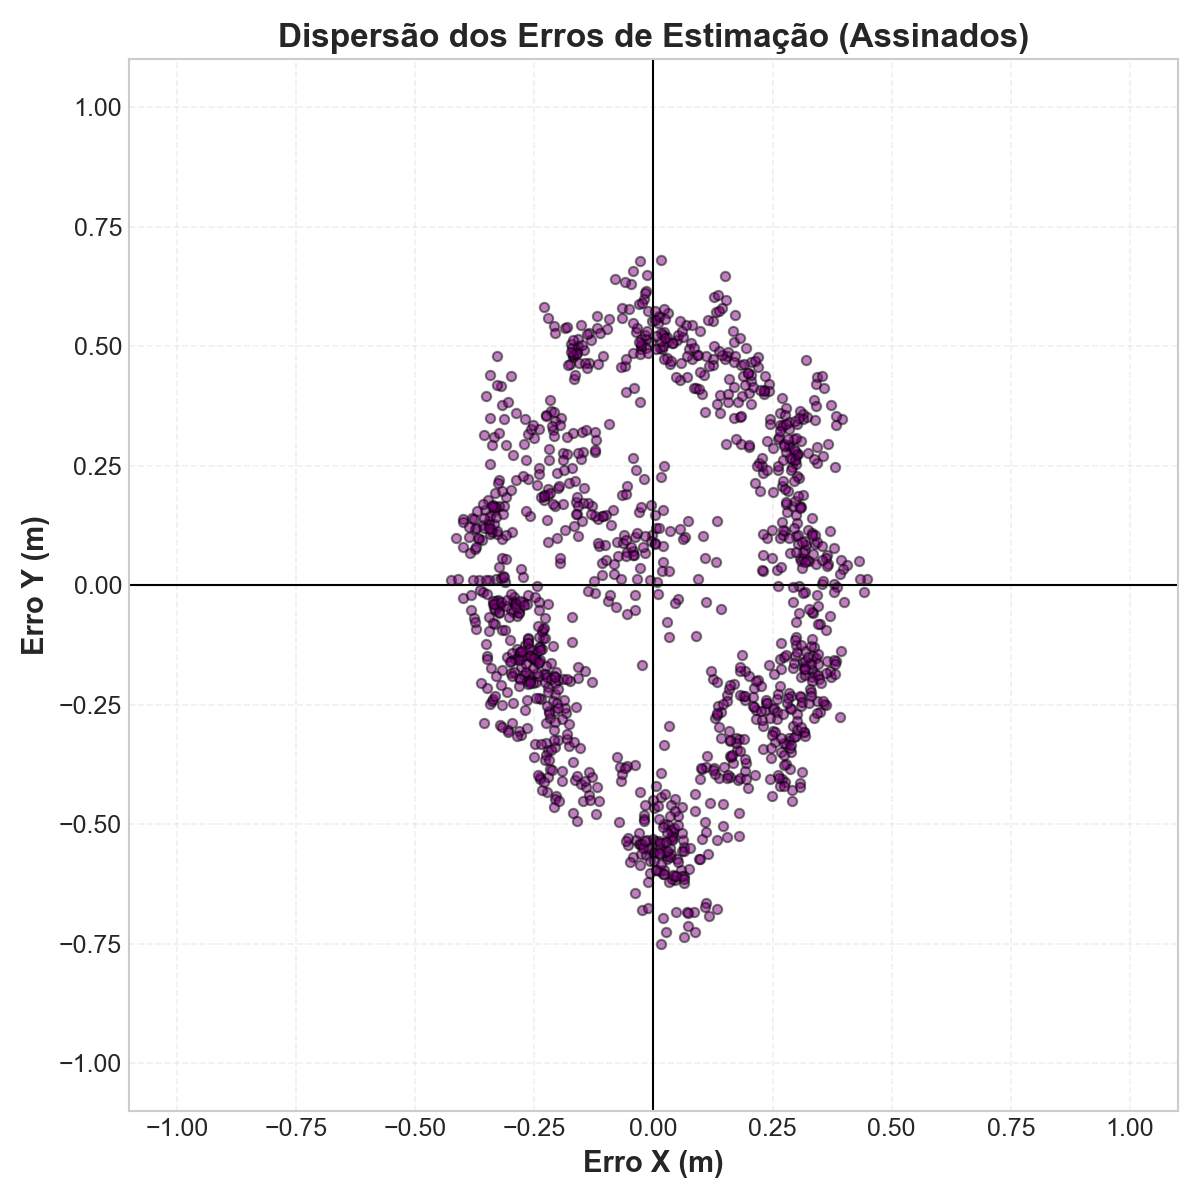
\includegraphics[width=\linewidth]{Figuras/C1/nsintonizado/simulacao_círculo_3_scatter.png}
        \vspace{1mm} \par {\small (a) Círculo}
    \end{minipage}
    \hfill
    \begin{minipage}[b]{0.24\linewidth}
        \centering
        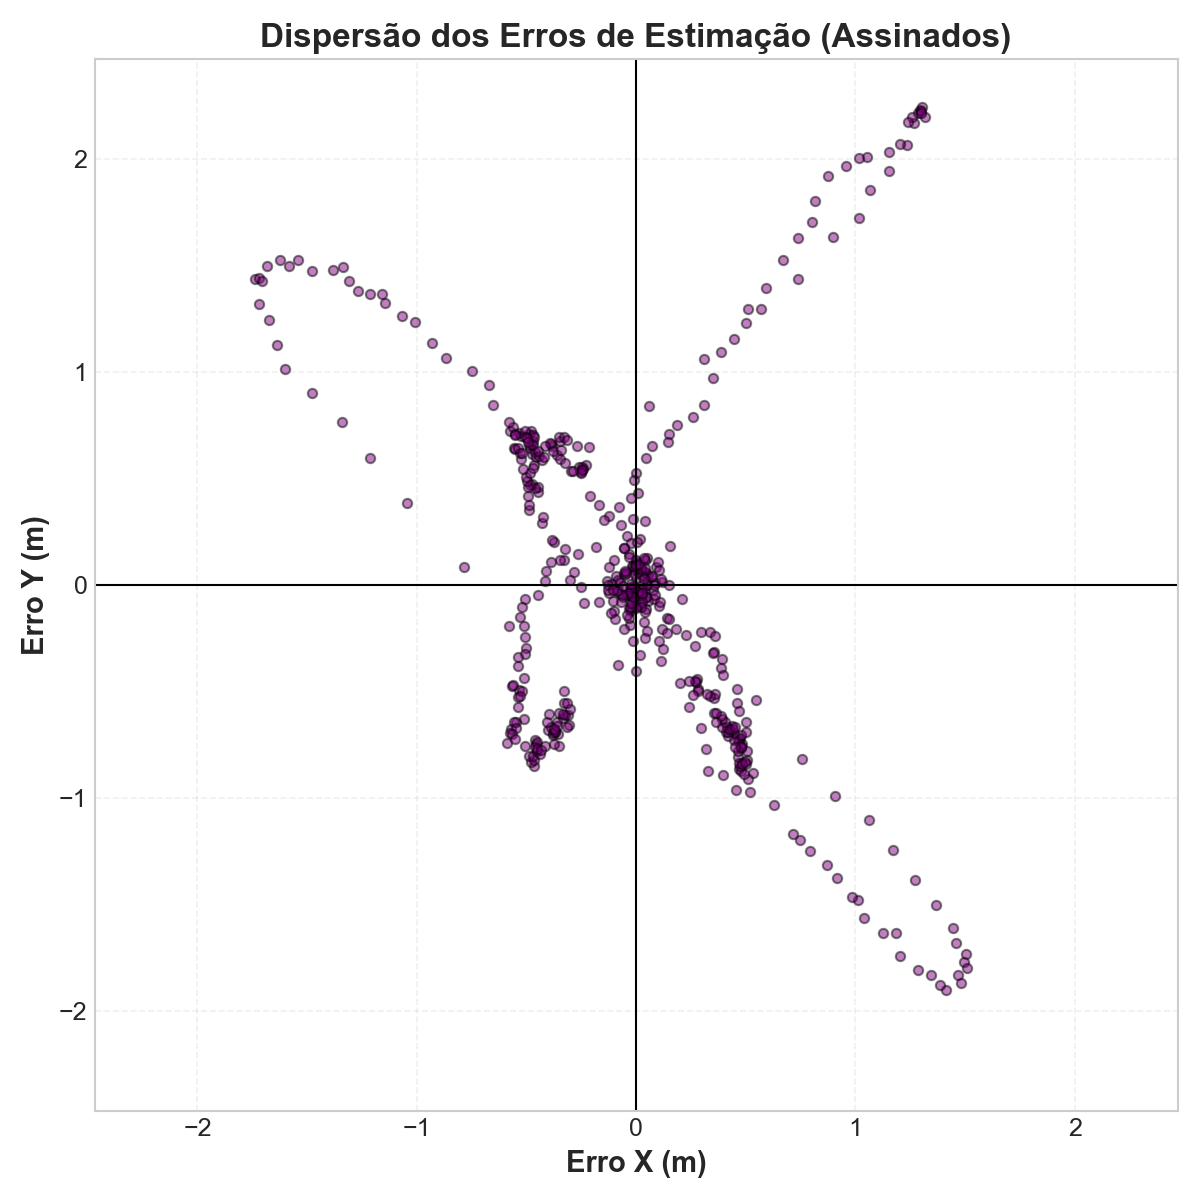
\includegraphics[width=\linewidth]{Figuras/C2/nsintonizado/simulacao_quadrado_3_scatter.png}
        \vspace{1mm} \par {\small (b) Quadrado}
    \end{minipage}
    \hfill
    \begin{minipage}[b]{0.24\linewidth}
        \centering
        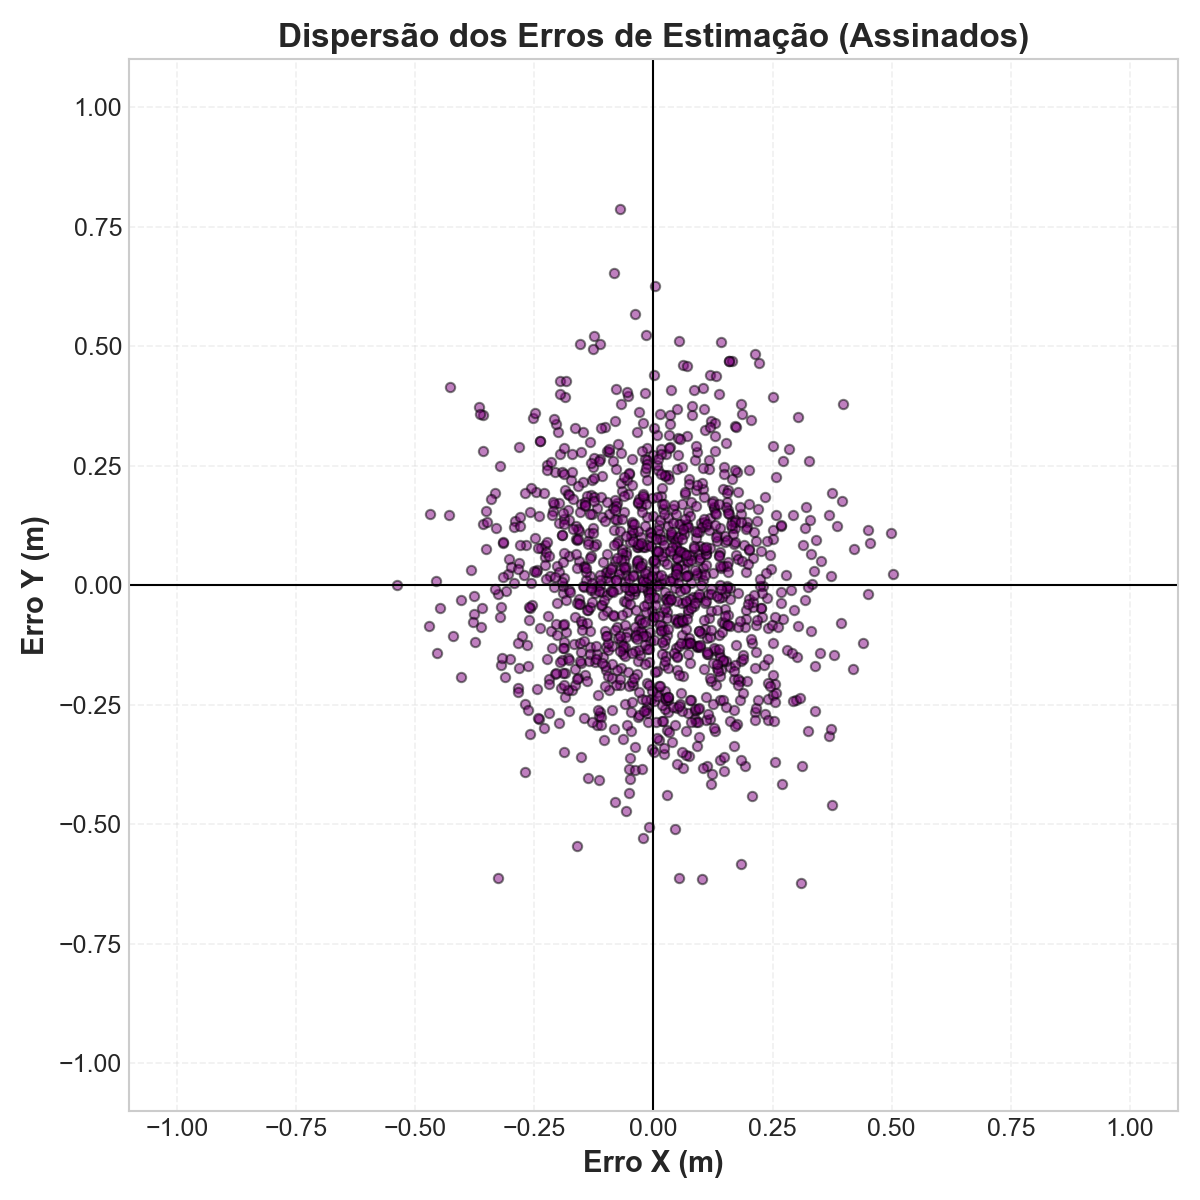
\includegraphics[width=\linewidth]{Figuras/C3/nsintonizado/simulacao_tangente_hiperbólica_3_scatter.png}
        \vspace{1mm} \par {\small (c) Tangente Hiperbólica}
    \end{minipage}
    
    \vspace{3mm}
    
    % Linha 2
    \begin{minipage}[b]{0.24\linewidth}
        \centering
        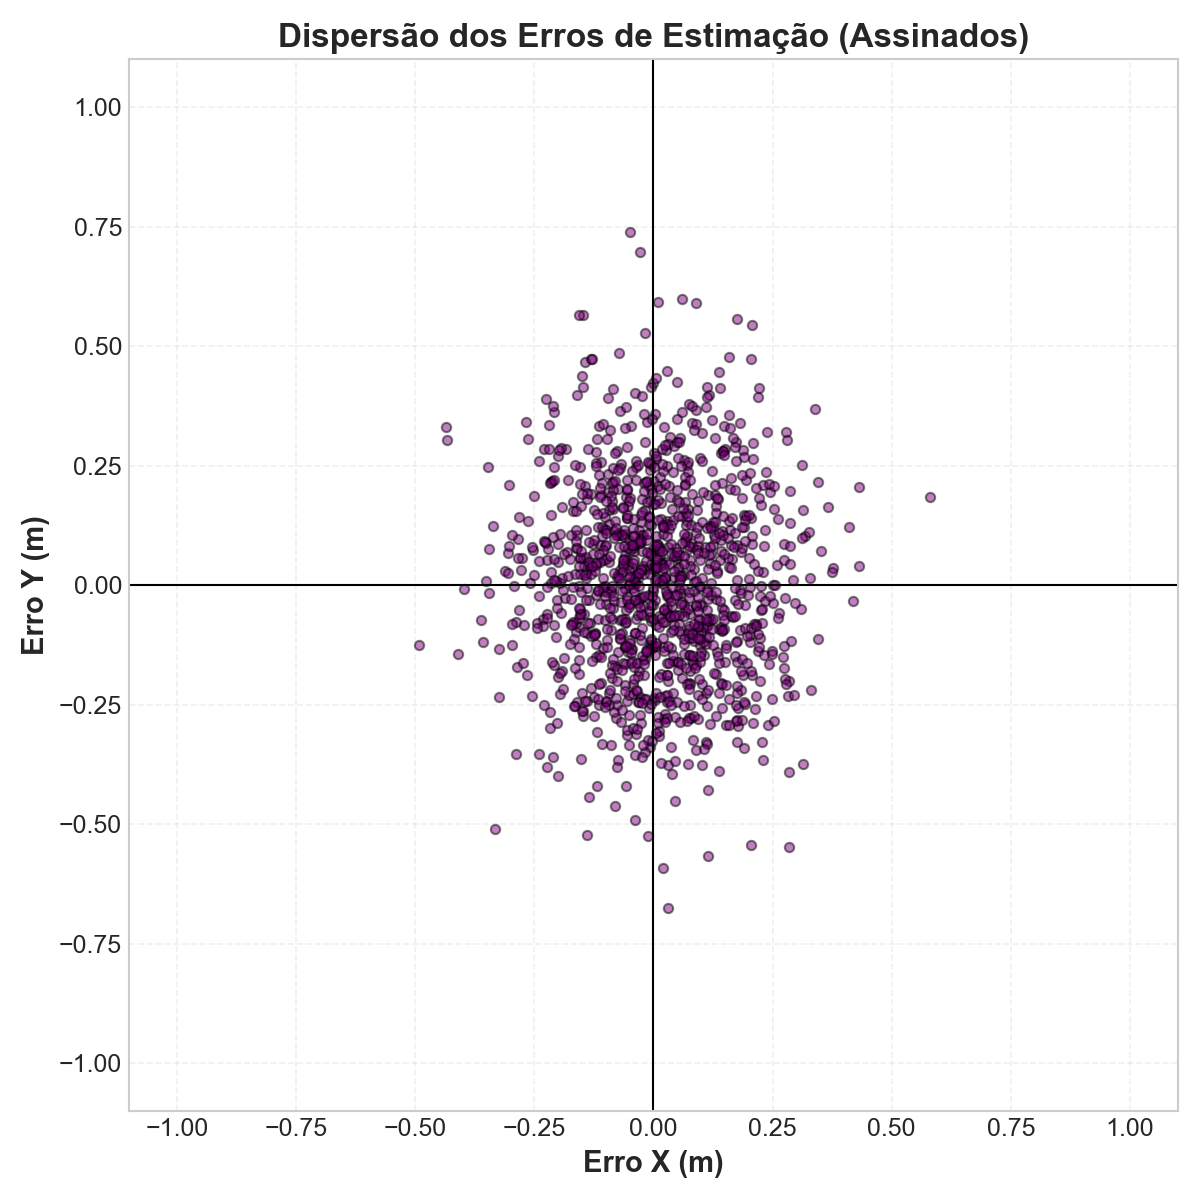
\includegraphics[width=\linewidth]{Figuras/C4/nsintonizado/simulacao_lemniscata_3_scatter.png}
        \vspace{1mm} \par {\small (d) Lemniscata}
    \end{minipage}
    \hfill
    \begin{minipage}[b]{0.24\linewidth}
        \centering
        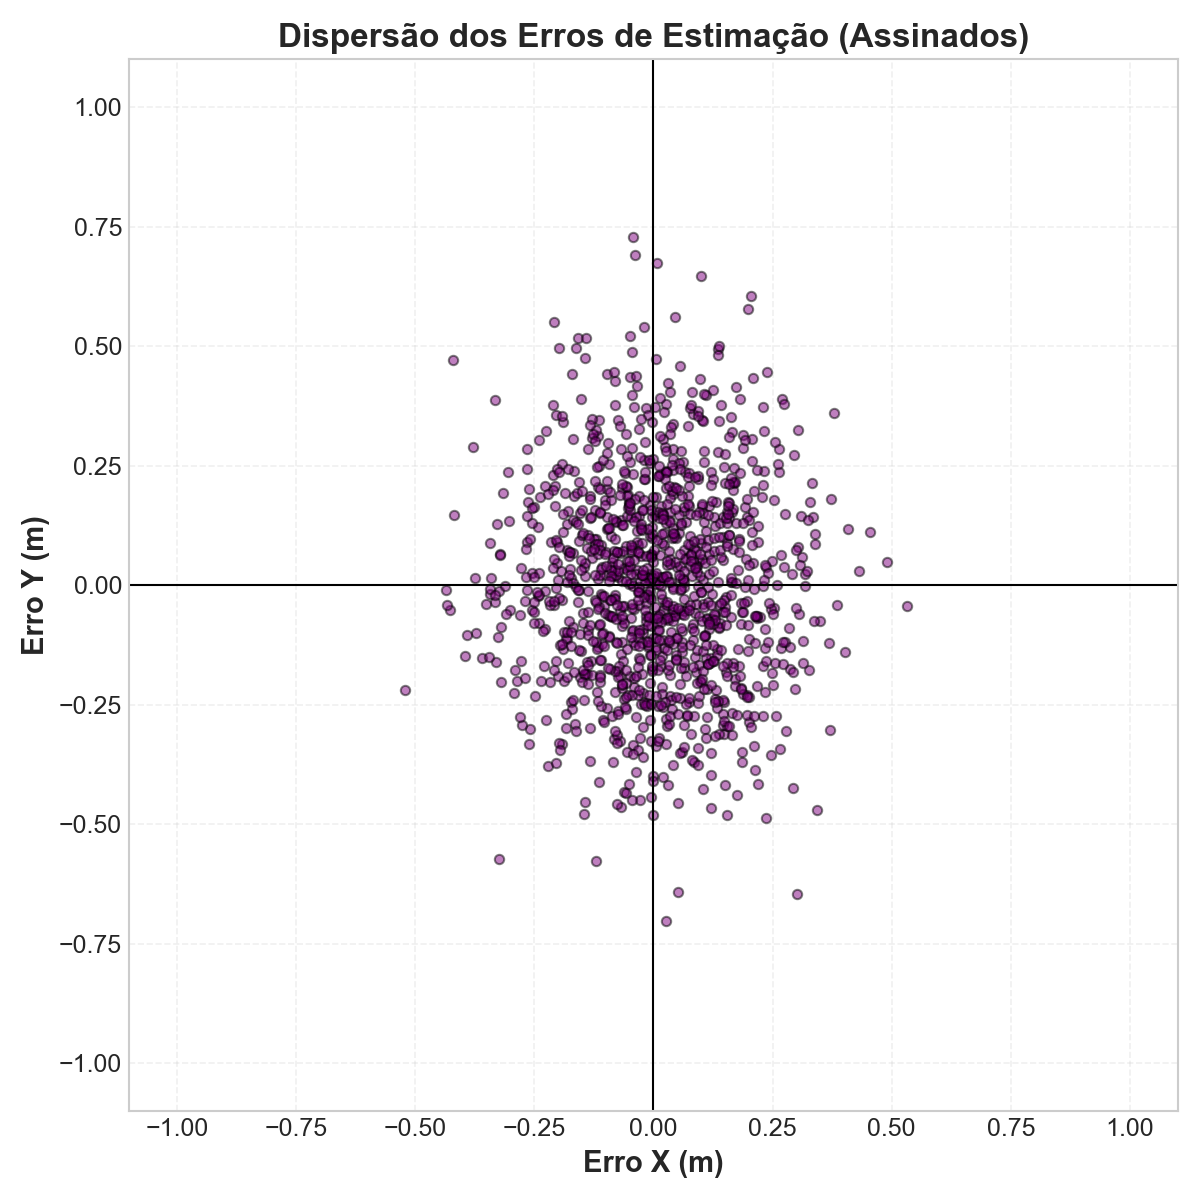
\includegraphics[width=\linewidth]{Figuras/C5/nsintonizado/simulacao_aleatória_3_scatter.png}
        \vspace{1mm} \par {\small (e) Aleatória}
    \end{minipage}
    \hfill
    \begin{minipage}[b]{0.24\linewidth}
        \centering
        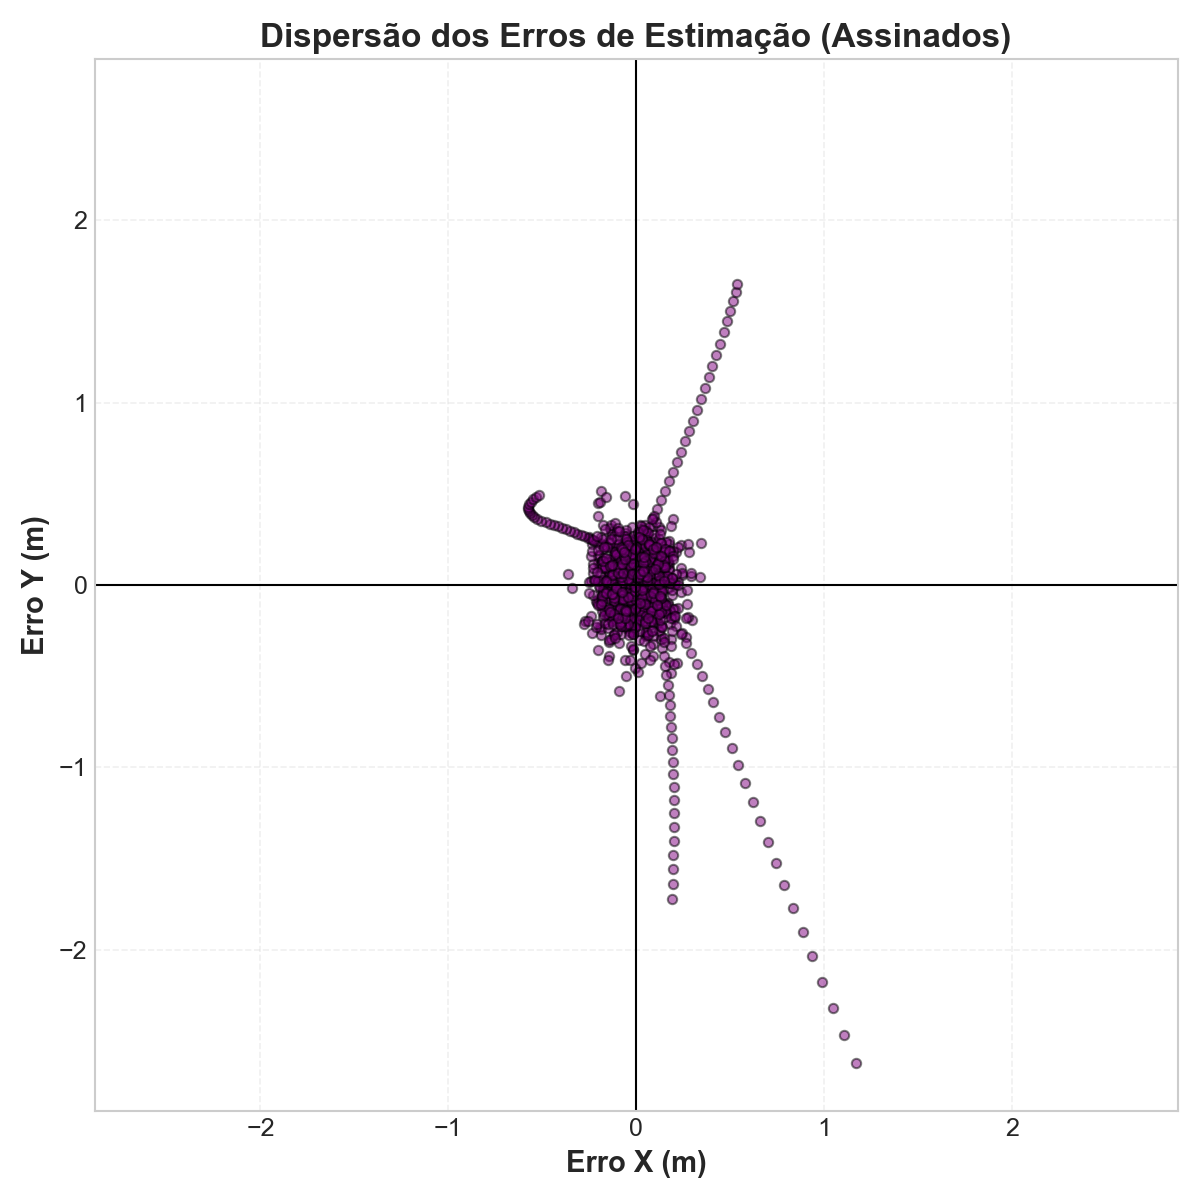
\includegraphics[width=\linewidth]{Figuras/C6/nsintonizado/simulacao_oclusão_3_scatter.png}
        \vspace{1mm} \par {\small (f) Oclusão}
    \end{minipage}

    \caption{Gráficos de dispersão das inovações para a \textbf{condição não sintonizada}. A dispersão irregular e o distanciamento acentuado da origem denotam a introdução de viés e a imprecisão preditiva do modelo.}
    \label{fig:app_scatter_naosintonizado_grid}
\end{figure*}


\end{document}